% A LaTeX template for MSc Thesis submissions to 
% Politecnico di Milano (PoliMi) - School of Industrial and Information Engineering
%
% S. Bonetti, A. Gruttadauria, G. Mescolini, A. Zingaro
% e-mail: template-tesi-ingind@polimi.it
%
% Last Revision: October 2021
%
% Copyright 2021 Politecnico di Milano, Italy. NC-BY

\documentclass{Configuration_Files/PoliMi3i_thesis}

%------------------------------------------------------------------------------
%	REQUIRED PACKAGES AND  CONFIGURATIONS
%------------------------------------------------------------------------------

% CONFIGURATIONS
\usepackage{parskip} % For paragraph layout
\usepackage{setspace} % For using single or double spacing
\usepackage{emptypage} % To insert empty pages
\usepackage{multicol} % To write in multiple columns (executive summary)
\setlength\columnsep{15pt} % Column separation in executive summary
\setlength\parindent{0pt} % Indentation
\raggedbottom  

\usepackage[utf8]{csquotes}

% PACKAGES FOR TITLES
\usepackage{titlesec}
% \titlespacing{\section}{left spacing}{before spacing}{after spacing}
\titlespacing{\section}{0pt}{3.3ex}{2ex}
\titlespacing{\subsection}{0pt}{3.3ex}{1.65ex}
\titlespacing{\subsubsection}{0pt}{3.3ex}{1ex}
\usepackage{color}

% PACKAGES FOR LANGUAGE AND FONT
\usepackage[english]{babel} % The document is in English  
\usepackage[utf8]{inputenc} % UTF8 encoding
\usepackage[T1]{fontenc} % Font encoding
\usepackage[11pt]{moresize} % Big fonts

% PACKAGES FOR IMAGES
\usepackage{graphicx}
\usepackage{transparent} % Enables transparent images
\usepackage{eso-pic} % For the background picture on the title page
\usepackage{subfig} % Numbered and caption subfigures using \subfloat.
\usepackage{tikz} % A package for high-quality hand-made figures.
\usetikzlibrary{}
\graphicspath{{./Images/}} % Directory of the images
\usepackage{caption} % Coloured captions
\usepackage{xcolor} % Coloured captions
\usepackage{amsthm,thmtools,xcolor} % Coloured "Theorem"
\usepackage{float}

% STANDARD MATH PACKAGES
\usepackage{amsmath}
\usepackage{amsthm}
\usepackage{amssymb}
\usepackage{amsfonts}
\usepackage{bm}
\usepackage[overload]{empheq} % For braced-style systems of equations.
\usepackage{fix-cm} % To override original LaTeX restrictions on sizes

% PACKAGES FOR TABLES
\usepackage{tabularx}
\usepackage{longtable} % Tables that can span several pages
\usepackage{colortbl}

% PACKAGES FOR ALGORITHMS (PSEUDO-CODE)
\usepackage{algorithm}
\usepackage{algorithmic}

% PACKAGES FOR REFERENCES & BIBLIOGRAPHY
\usepackage[colorlinks=true,linkcolor=black,anchorcolor=black,citecolor=black,filecolor=black,menucolor=black,runcolor=black,urlcolor=black]{hyperref} % Adds clickable links at references
\usepackage{cleveref}
\usepackage[square, numbers]{natbib} % Square brackets, citing references with numbers, citations sorted by appearance in the text and compressed
\bibliographystyle{abbrvnat} % You may use a different style adapted to your field

% OTHER PACKAGES
\usepackage{pdfpages} % To include a pdf file
\usepackage{afterpage}
\usepackage{lipsum} % DUMMY PACKAGE
\usepackage{fancyhdr} % For the headers
\fancyhf{}

% Input of configuration file. Do not change config.tex file unless you really know what you are doing. 
% Define blue color typical of polimi
\definecolor{bluepoli}{cmyk}{0.4,0.1,0,0.4}

% Custom theorem environments
\declaretheoremstyle[
  headfont=\color{bluepoli}\normalfont\bfseries,
  bodyfont=\color{black}\normalfont\itshape,
]{colored}

% Set-up caption colors
\captionsetup[figure]{labelfont={color=bluepoli}} % Set colour of the captions
\captionsetup[table]{labelfont={color=bluepoli}} % Set colour of the captions
\captionsetup[algorithm]{labelfont={color=bluepoli}} % Set colour of the captions

\theoremstyle{colored}
\newtheorem{theorem}{Theorem}[chapter]
\newtheorem{proposition}{Proposition}[chapter]

% Enhances the features of the standard "table" and "tabular" environments.
\newcommand\T{\rule{0pt}{2.6ex}}
\newcommand\B{\rule[-1.2ex]{0pt}{0pt}}

% Pseudo-code algorithm descriptions.
\newcounter{algsubstate}
\renewcommand{\thealgsubstate}{\alph{algsubstate}}
\newenvironment{algsubstates}
  {\setcounter{algsubstate}{0}%
   \renewcommand{\STATE}{%
     \stepcounter{algsubstate}%
     \Statex {\small\thealgsubstate:}\space}}
  {}

% New font size
\newcommand\numfontsize{\@setfontsize\Huge{200}{60}}

% Title format: chapter
\titleformat{\chapter}[hang]{
\fontsize{50}{20}\selectfont\bfseries\filright}{\textcolor{bluepoli} \thechapter\hsp\hspace{2mm}\textcolor{bluepoli}{|   }\hsp}{0pt}{\huge\bfseries \textcolor{bluepoli}
}

% Title format: section
\titleformat{\section}
{\color{bluepoli}\normalfont\Large\bfseries}
{\color{bluepoli}\thesection.}{1em}{}

% Title format: subsection
\titleformat{\subsection}
{\color{bluepoli}\normalfont\large\bfseries}
{\color{bluepoli}\thesubsection.}{1em}{}

% Title format: subsubsection
\titleformat{\subsubsection}
{\color{bluepoli}\normalfont\large\bfseries}
{\color{bluepoli}\thesubsubsection.}{1em}{}

% Shortening for setting no horizontal-spacing
\newcommand{\hsp}{\hspace{0pt}}

\makeatletter
% Renewcommand: cleardoublepage including the background pic
\renewcommand*\cleardoublepage{%
  \clearpage\if@twoside\ifodd\c@page\else
  \null
  \AddToShipoutPicture*{\BackgroundPic}
  \thispagestyle{empty}%
  \newpage
  \if@twocolumn\hbox{}\newpage\fi\fi\fi}
\makeatother

%For correctly numbering algorithms
\numberwithin{algorithm}{chapter}

%----------------------------------------------------------------------------
%	NEW COMMANDS DEFINED
%----------------------------------------------------------------------------

% EXAMPLES OF NEW COMMANDS
\newcommand{\bea}{\begin{eqnarray}} % Shortcut for equation arrays
\newcommand{\eea}{\end{eqnarray}}
\newcommand{\e}[1]{\times 10^{#1}}  % Powers of 10 notation

%----------------------------------------------------------------------------
%	ADD YOUR PACKAGES (be careful of package interaction)
%----------------------------------------------------------------------------

%----------------------------------------------------------------------------
%	ADD YOUR DEFINITIONS AND COMMANDS (be careful of existing commands)
%----------------------------------------------------------------------------

%----------------------------------------------------------------------------
%	BEGIN OF YOUR DOCUMENT
%----------------------------------------------------------------------------

\begin{document}

\fancypagestyle{plain}{%
\fancyhf{} % Clear all header and footer fields
\fancyhead[RO,RE]{\thepage} %RO=right odd, RE=right even
\renewcommand{\headrulewidth}{0pt}
\renewcommand{\footrulewidth}{0pt}}

%----------------------------------------------------------------------------
%	TITLE PAGE
%----------------------------------------------------------------------------

\pagestyle{empty} % No page numbers
\frontmatter % Use roman page numbering style (i, ii, iii, iv...) for the preamble pages

\puttitle{
	title=Title, % Title of the thesis
	name=Matteo Regge and Manuel Stoppiello, % Author Name and Surname
	course=Xxxxxxx Engineering - Ingegneria Xxxxxxx, % Study Programme (in Italian)
	ID  = 10619213,  % Student ID number (numero di matricola)
	advisor= Prof. Maurizio Magarini, % Supervisor name
	coadvisor={Antonio Coviello}, % Co-Supervisor name, remove this line if there is none
	academicyear={2023-24},  % Academic Year
} % These info will be put into your Title page 

%----------------------------------------------------------------------------
%	PREAMBLE PAGES: ABSTRACT (inglese e italiano), EXECUTIVE SUMMARY
%----------------------------------------------------------------------------
\startpreamble
\setcounter{page}{1} % Set page counter to 1

% ABSTRACT IN ENGLISH
\chapter*{Abstract} 
Here goes the Abstract in English of your thesis followed by a list of keywords.
The Abstract is a concise summary of the content of the thesis (single page of text)
and a guide to the most important contributions included in your thesis.
The Abstract is the very last thing you write.
It should be a self-contained text and should be clear to someone who hasn't (yet) read the whole manuscript.
The Abstract should contain the answers to the main scientific questions that have been addressed in your thesis.
It needs to summarize the adopted motivations and the adopted methodological approach as                          well as the findings of your work and their relevance and impact.
The Abstract is the part appearing in the record of your thesis inside POLITesi,
the Digital Archive of PhD and Master Theses (Laurea Magistrale) of Politecnico di Milano.
The Abstract will be followed by a list of four to six keywords.
Keywords are a tool to help indexers and search engines to find relevant documents.
To be relevant and effective, keywords must be chosen carefully.
They should represent the content of your work and be specific to your field or sub-field.
Keywords may be a single word or two to four words. 
\\
\\
\textbf{Keywords:} here, the keywords, of your thesis % Keywords

% ABSTRACT IN ITALIAN
\chapter*{Abstract in lingua italiana}
Qui va l'Abstract in lingua italiana della tesi seguito dalla lista di parole chiave.
\\
\\
\textbf{Parole chiave:} qui, vanno, le parole chiave, della tesi % Keywords (italian)

%----------------------------------------------------------------------------
%	LIST OF CONTENTS/FIGURES/TABLES/SYMBOLS
%----------------------------------------------------------------------------

% TABLE OF CONTENTS
\thispagestyle{empty}
\tableofcontents % Table of contents 
\thispagestyle{empty}
\cleardoublepage

%-------------------------------------------------------------------------
%	THESIS MAIN TEXT
%-------------------------------------------------------------------------
% In the main text of your thesis you can write the chapters in two different ways:
%
%(1) As presented in this template you can write:
%    \chapter{Title of the chapter}
%    *body of the chapter*
%
%(2) You can write your chapter in a separated .tex file and then include it in the main file with the following command:
%    \chapter{Title of the chapter}
%    \input{chapter_file.tex}
%
% Especially for long thesis, we recommend you the second option.

\addtocontents{toc}{\vspace{2em}} % Add a gap in the Contents, for aesthetics
\mainmatter % Begin numeric (1,2,3...) page numbering

% --------------------------------------------------------------------------
% NUMBERED CHAPTERS % Regular chapters following
% --------------------------------------------------------------------------
\chapter{Introduction}
\section{PNRelay project}
Peripheral nerves injuries (PNI) are a significant cause of morbidity and disability today,
they affect almost 20 milions in the USA alone, and deeply damage both the physical and psychological well-being of those who suffer from these injuries. \cite{zhangResearchHotspotsTrends2022}
The loss of functionality is caused by the damage of the nervous systems pathways that connect the brain to peripheral parts of the body.
Moreover PNI's receive a poor prognosis since the regenerative capabilities of the nervous systems are limited and slow.

Recently, though there have been promising works of reserach in neuroscience that aim at improving the well-being of people that suffer from PNI by developing implanted devices that can connect to the Pheripheral Nervous System (PNS).
In particular, bi-directional interfaces have the goal to restore the communication between the brain and the peripheral area whose sensorimotor feedback has been lost, effectively restoring the nervous pathways that have been damaged.
This kind of interfaces can be realized with nerve electrodes that are installed chirurgically and can measure the voltage of a certain nerve and assess its signal or stimulate them directly.
In this deeply interesting and thriving area of research it has emerged the PNRelay project 
which has been presented as a collaboration effort between the Politecnico di Milano and the Politecnico di Torino and has the objective to target PNI related issues by developing a new peripheral nerve interface, capable of conveying information between brain and body peripherical areas.
In particular, this interface has the goal to register the nerve electrical signal, send it to a computer so that it can be interpreted and classified via a deep learning model and then stimulate the right nerves in order to elicit the corresponding movement.
Although muscle stimulation has not yet been incorporated, it remains a pivotal area for future exploration and development.
The project is targeted for preclinical trials on rats and in particular, injuries to the sciatic nerve, but it nontheless has great potential for future clinical applications.
The recorded signal thanks to the electrode is known as  Electroneurography (ENG) signal
which has the potential to provide a valuable control signal for closed-loop neuroprostheses [5] (from davide)
'''davide'''
Other biological signals have been used with the aim of restoring PNI. Electromyography,
(EMG) signals from muscle activity and Electroencephalogram (EEG) signals reflecting brain activity are used in restoring limb function. EMG signals decode control commands for powered upper-limb prostheses, facilitating dexterity and mobility, but the acquisition and use of such myosignals are cumbersome and complicated [12]–[14]. EEG signals can be used to decipher user intent, driving neuroprosthetic devices to restore lost limb functionality. In recent studies, these signals are used to examine the functions and movements behavior of humans [15], [16].
'''davide'''


The device that has been engineered as part of the PNRelay is made of two main subparts:
one that is implanted and one that is external.
\\
The internal implant is composed of different parts: the cuff electrodes to acquire the signal, the Senseback ASIC chip, wrapped in a biocompatible capsuel, that is required for the processing of the singal and a transdermal port for the powering of the wireless device.

% copied from davide
Extra-neural cuff electrodes, positioned externally on the nerve’s surface, are chosen for their lower invasiveness in acquiring ENG data [20]. The data transmission module, which is responsible for data signal processing, is currently being developed for full-body integration. The external component hosts the classifier, which by performing an online operation, allows the different stimuli to be recognized. The signal is then sent to the stimulator, which proceeds to close the loop. The overall scheme for animal testing is shown in Figure 1.1. During initial experimental phases, the classifier may operate on a computer connected to the external circuit, with the ultimate objective being its integration into the implanted circuitry. Due to the typically substan- tial variations in neurological data among individuals, classification algorithms in this domain are often tailored to specific subjects [3]. This further compounds the challenge of gathering a sufficient amount of biological data on same subject. Challenges persist in decoding neural signal information due to limitations imposed by acquisition invasiveness. While extra-neural cuff electrodes represent a less invasive option for chronic implantation [21], the classification of sensory stimuli recorded through them remains complex due to a limited SNR. Various techniques have been explored to address this challenge [22]–[24], but the optimal classification approach remains an open area for further research and exploration.
% copied from davide
\\
\subsection{PNRelay Setup}

\subsection{PNRelay functionality (chiara objectives)}



\subsection{Ethical concerns}

\subsection{Thesis outline}


Our master's thesis endeavors to provide a comprehensive understanding of the research project's scope and objectives, aiming to delve into various facets of the subject matter. In Chapter 2, we lay the foundation by presenting the necessary background information essential for contextualizing our study. Moving forward, Chapter 3 offers a detailed exploration of the current state-of-the-art of the topics incorporated in our work, offering insights into the existing research landscape.

In Chapter 4 we delineate our methodology, detailing the approach undertaken to conduct our research. Here, we expound upon the materials utilized and outline the practical implementations of our project. Moreover, this chapter serves as a platform to showcase our contribution to the PNRelay project, elucidating the innovative approaches and methodologies we have introduced.

Transitioning to Chapter 5, we present the results derived from our efforts, providing a comprehensive analysis and discussion of the outcomes obtained. Through an in-depth examination, we elucidate the implications and significance of our findings, shedding light on the potential benefits and applications of our endeavors. This chapter also serves as a repository of the data that underpins our conclusions, offering insights into future directions and avenues for further exploration within the realm of PNRelay.

Finally, Chapter 6 marks the culmination of our thesis, wherein we encapsulate the essence of our research journey. Here, we provide a reflective summary of our contribution, acknowledging both the strengths and limitations of our work. Furthermore, we offer insights into potential areas of improvement and future iterations, paving the way for continued advancements in the field.





\chapter{Background}

In this section, we will present an outline of the information transmission process within the nervous system, particularly emphasizing the conveyance of sensory data. The objective is to gain insight into the operational flow of our project and to grasp the attributes of the signal requiring transmission. Additionally, we will delve into the distinctive features of ENG signals and the significance of extra-neural cuff electrodes, as they play pivotal roles in data acquisition for transmission purposes.

\section{Nervous Systems}

The nervous system orchestrates an organism's activities and ensures seamless communication throughout the body. In vertebrates, it is divided into two primary components: the central nervous system (CNS) and the peripheral nervous system (PNS). The CNS, consisting of the brain and spinal cord, acts as the main processing hub, whereas the PNS includes nerves that branch out from the CNS to various parts of the body.

On a cellular scale, the nervous system is distinguished by its specialized nerve cells, known as neurons. These neurons are equipped with unique features that facilitate the rapid and precise transmission of signals to other cells. These signals travel as electrochemical waves along slender fibers called axons, leading to the release of neurotransmitters at synapses—the contact points between neurons. In addition to neurons, the nervous system encompasses glial cells, or glia, which offer structural and metabolic support. Recent studies indicate that glia may also have important roles in signaling processes.
'''need to rewrite"""
'''add neurons picture'''

\subsection{Central nervous system}

The central nervous system (CNS) is essential for processing sensory information from the peripheral nervous system (PNS) and integrating it to form appropriate responses. It generates motor responses, coordinates voluntary movements, and manages reflex actions. The CNS also governs higher cognitive functions and emotions, maintains homeostasis, facilitates learning and memory, processes sensory inputs, and controls autonomic functions such as heart rate and digestion. Through these roles, the CNS ensures the organism's ability to perceive, respond, and adapt to its environment while maintaining internal stability.
It consist of two main parts: the brain and the spinal cord.
The brain is housed inside the cranium and is responsible for all the main functions of the brain, while the spinal cord can be found inside the vertebral column and is crucial in linking the CNS to the PNS, allowing the transmission of motor commands from the brain to the rest of the body and the sensory information back to the brain.
The spinal cord is also responsible for reflexes, unconcious responses to quick or unexpected stimuli.


\subsection{Peripheral nervous system}

Since the PNRelay aims at elicitng motor stimulation by transmitting electrical signals through the body is of the utmost importance that we well understand how our nervous system propagates signals.
The Peripheral Nervous System comprises all the network structures apart from the brain and the spinal cord that instead form the CNS as described above.
Its purpose is to propagate nervous signals to every corner of our body and handle the subsequent motor responses.
It is how our organism sends information to the brain (CNS) and how, vice-versa, sends the responses to the rest of the body in the opposite direction.

Despite the complexity just described, the Peripheral Nervous System is composed of two types of cell:

\begin{itemize}

	\item  Neurons: cells that conduct impulses inside the NS.
	\item Glial cells: these are nonconductive cells and provide a support system for
	neurons protecting them.
\end{itemize}



\section{Implanted medical devices normative and regulation}

In order to have a medical implanted device, such as the one taken into consideration in this thesis work, it should respect the premarket standards for the specific location where the device is intended to be approved, various organizations co-operate to guarantee the best standards \cite{} 1 . In particular, the responsible authorities are Food and Drugs Administration in the United State (USA) and European Commission (CE) in the European Union (EU). 
The normative given by these authorities are necessary to guarantee safeness of the patient and a lower grade of risk for the patient who will use the specific medical device, considering for each one the trade off between risks and benefits, together with the ensure of efficiency of medical devices.

\subsection{FDA}

FDA administration subdivides the medical devices that should be evaluated and approved into three classes of risks, based on the specific application. Up to now, more than 1700 different devices have been classified and divided into the specific class. \cite{healthClassifyYourMedical2023}
The classes of risk that FDA utilizes and their relative needs to be approved are the following ones: 
\begin{itemize}

	\item  Class I (General Controls): This class can be subdivided into two subclasses: with exe        t4mptions and without exemptions.
	\item  Class II (General Controls and Special Controls): this class can also be subdivided into the two subclasses with and without exemptions.
	\item  Class III (General Controls and Premarket Approval)

\end{itemize}

The class is assigned to a specific device basing on a risk based approach, the more the device can be dangerous for the patient, the highest would be the class of risk and as a consequence, the more selective would be the approval practice. For what concern Class I and Class II a 510k is required. Class III is the only one which is subject to premarket approval (PMA), unless the device were on the market before the medical amendments in 1976, in which case a 510k could be sufficient.
To determine the classification of the device for FDA it is possible to consult the device specific device panel \cite{healthDeviceClassificationPanels2023} which best describes the product in analysis. For Senseback, the specific device panel is the one related to neurology. Specifically, the one which best fits the intended use is the 882.5870 “Implanted peripheral nerve stimulator for pain relief” \cite{CFRCodeFederal} which makes Senseback falls into the Class of risk II.
In order to understand how FDA values the biocompatibility of the devices with the body, standard iso 10993, in particular 10093-1 \cite{14:00-17:00ISO1099312018a} should be taken into account. Recently, on September 8 2023, FDA has published a guidance \cite{healthUseInternationalStandard2023} which explicit how to use this standard for a biological evaluation during the design of medical devices. 
ISO 10993-1 and FDA guidance
ISO is an independent, non-governmental international organization \cite{ISOInternationalOrganization}. It provides standards to guarantee to the user that products are safe as much as possible, providing guidance for each step of design and premarket of the device in analysis.
The standard ISO 10993-1 focuses on the categorization of medical devices basing on the duration and the nature of contact, both for implanted and external devices.
The flow charts reported in Figure 1 and in Figure 2 reports how to proceed for a biocompatibility evaluation.

\begin{figure}[H]
	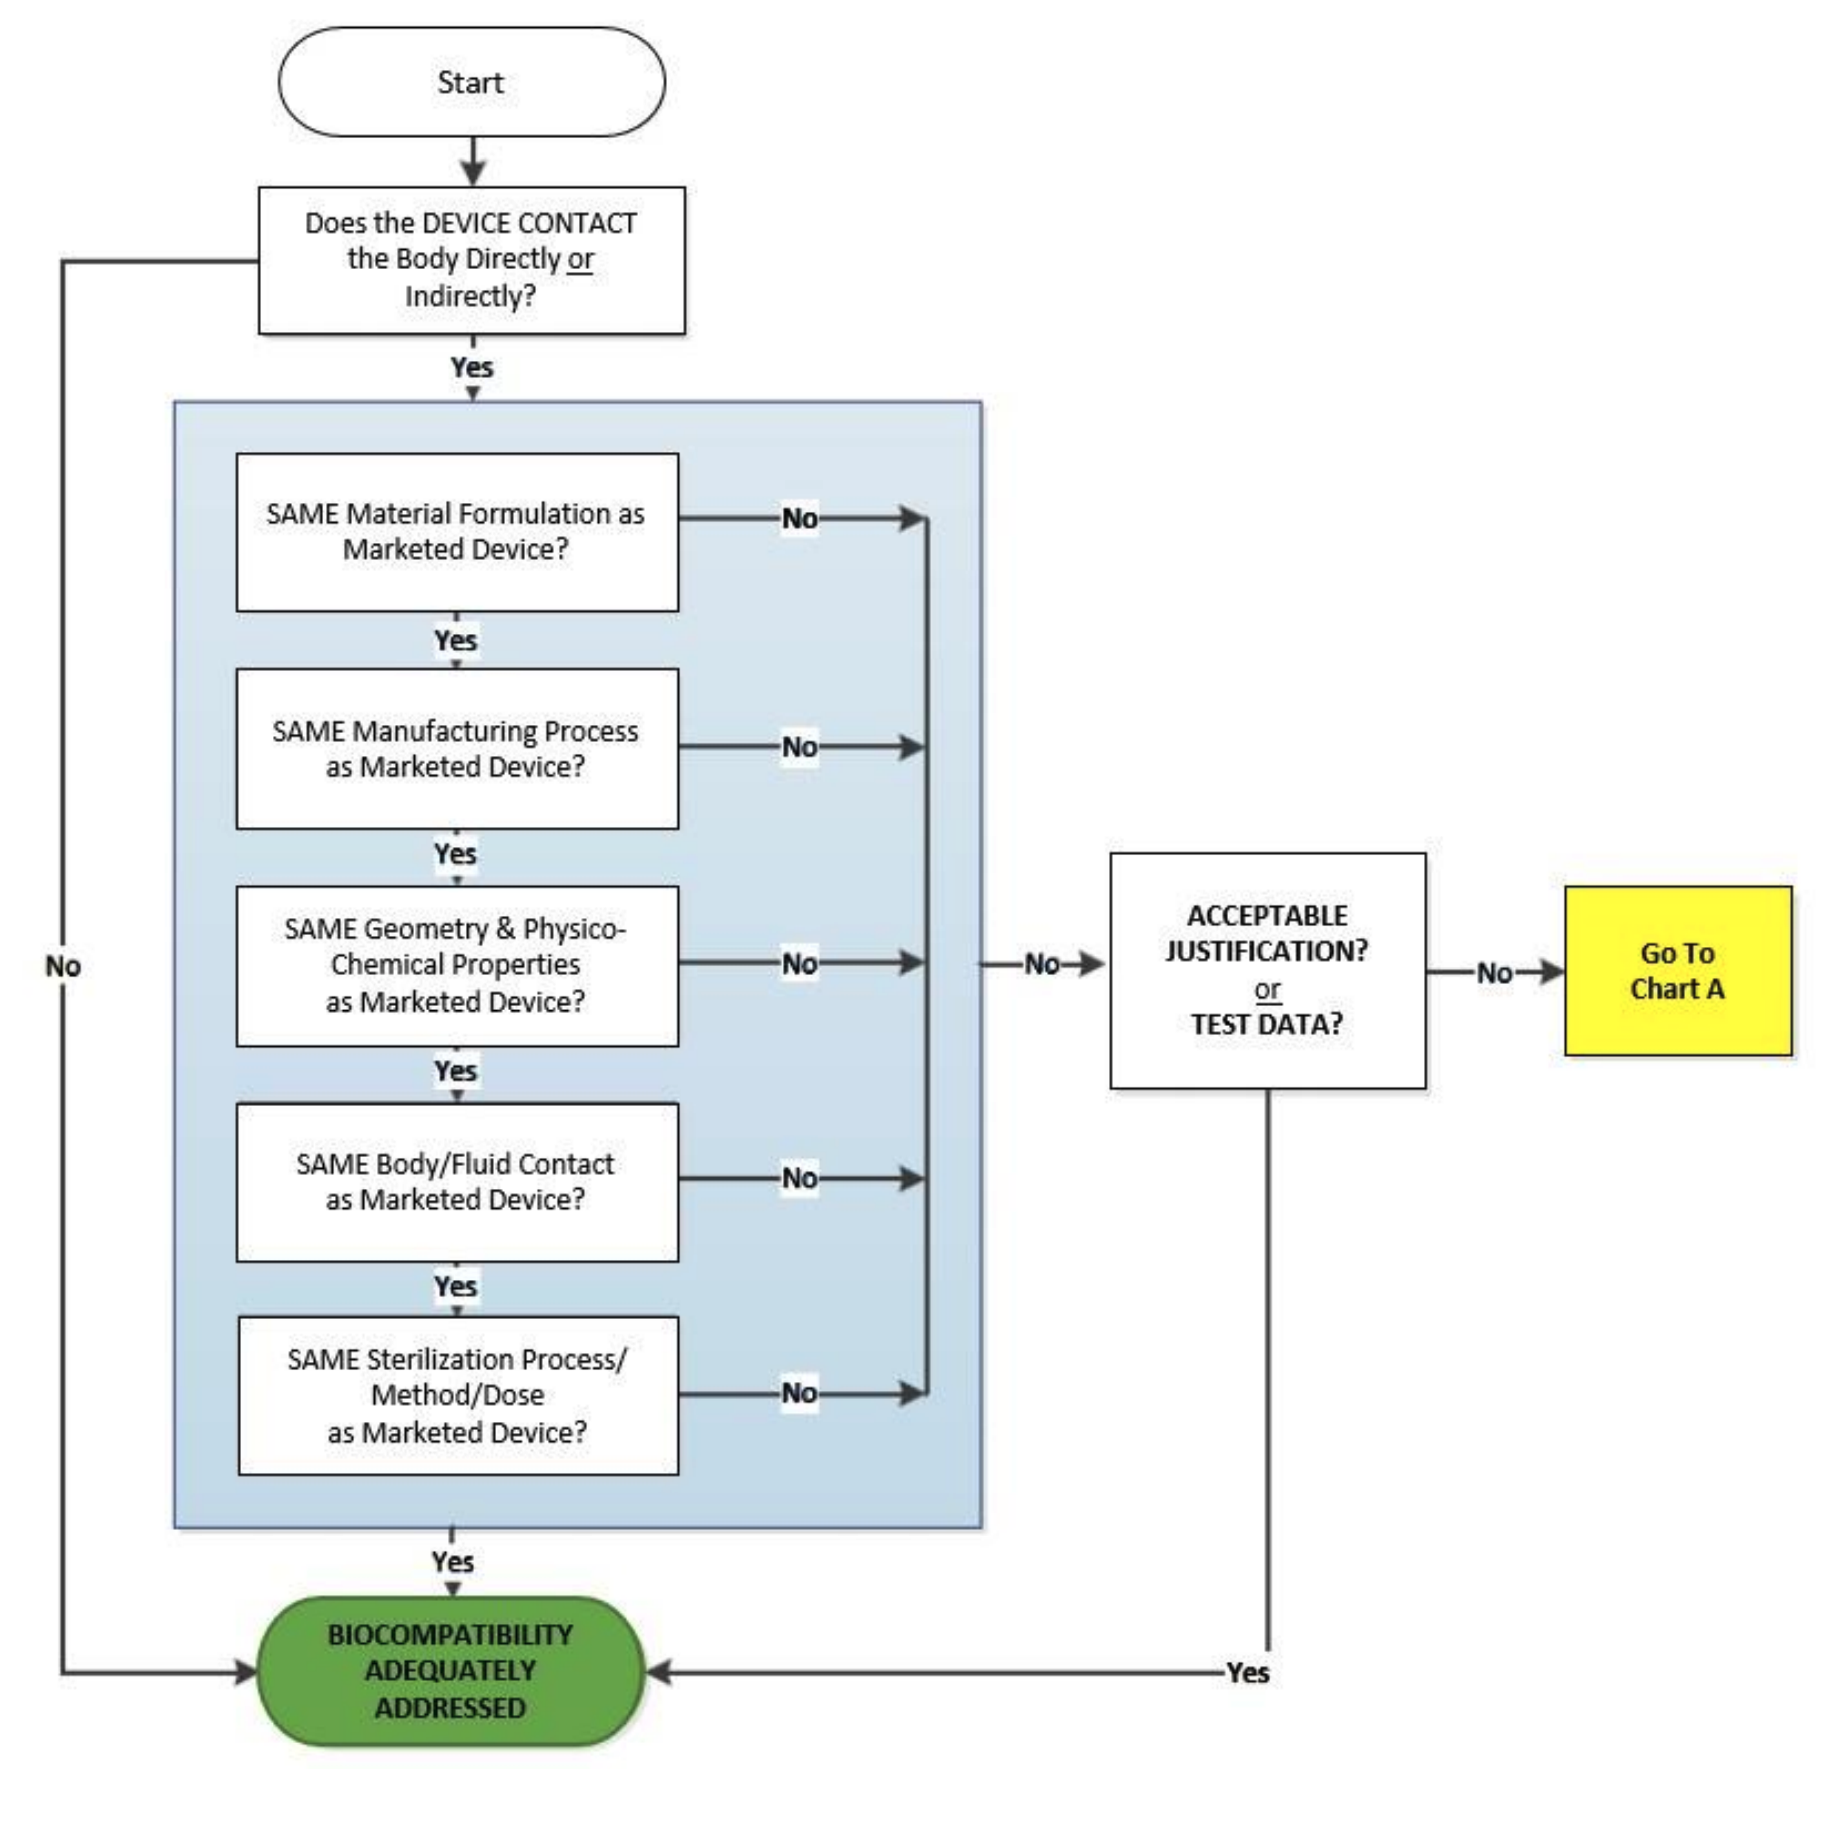
\includegraphics[scale=0.4]{figure1_fda.png}
	\centering
\end{figure}
\begin{figure}[H]

	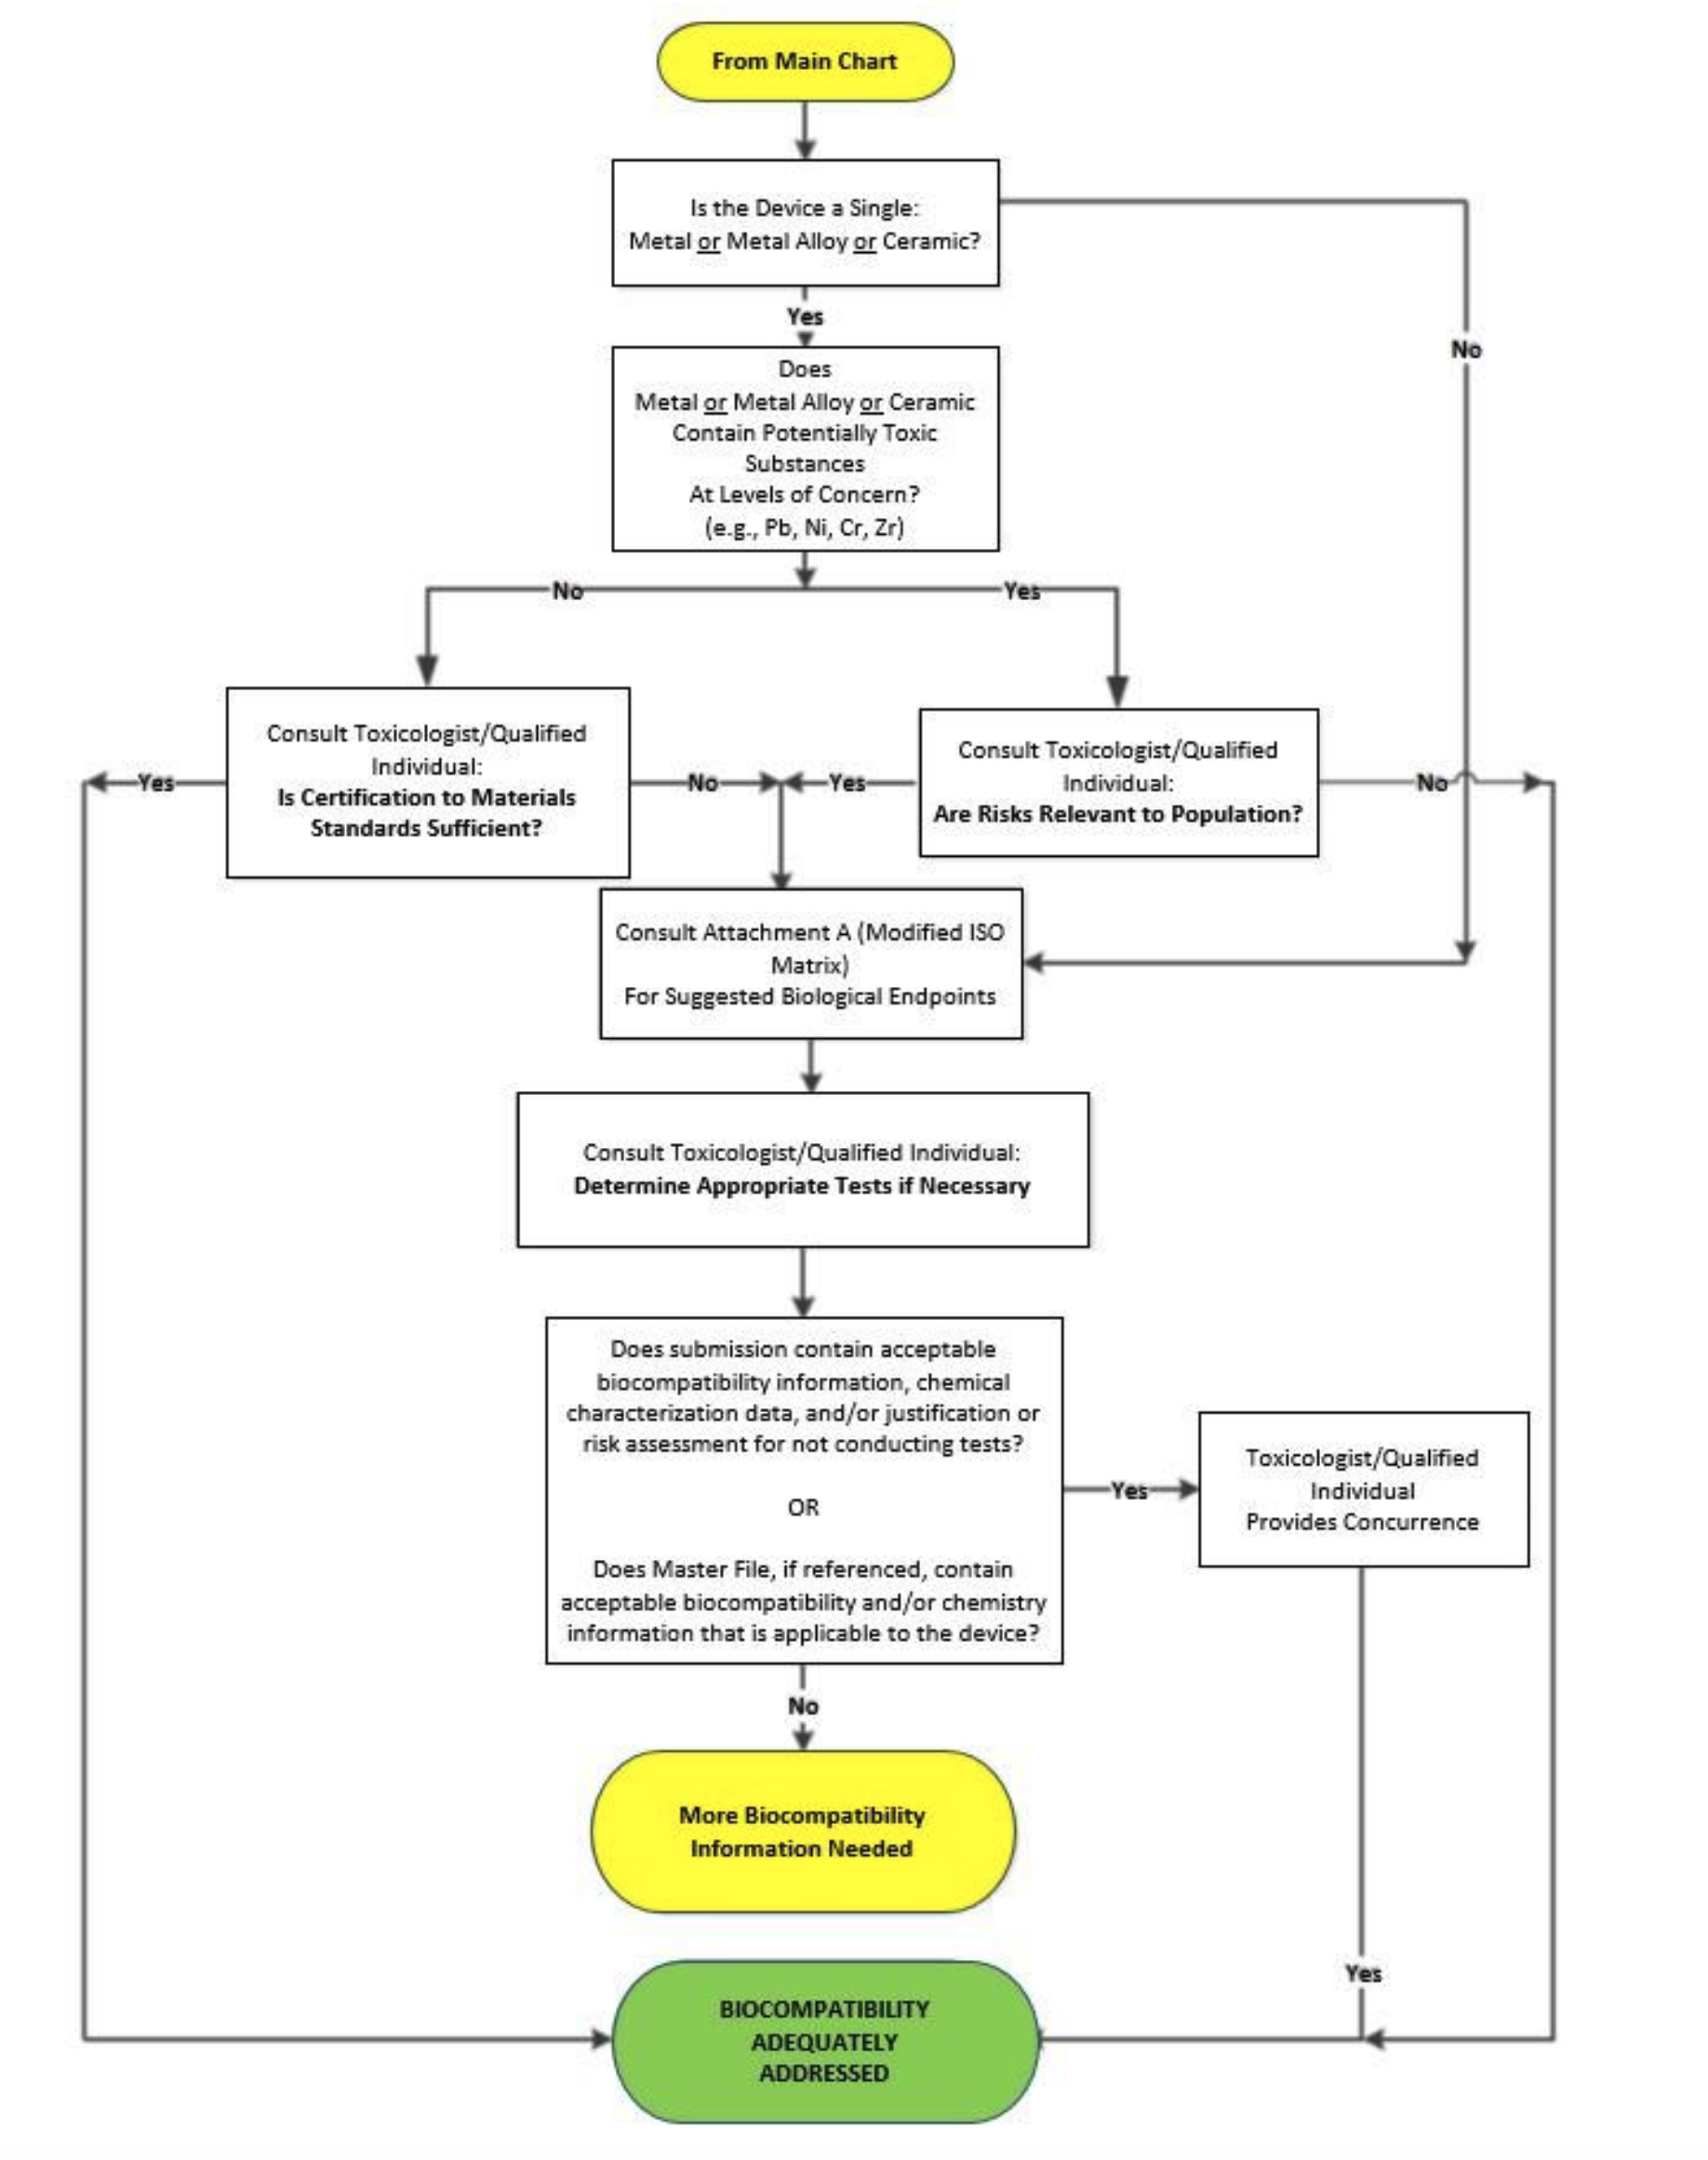
\includegraphics[scale=0.3]{figure2_fda.png}
	\centering
\end{figure}





As it is possible to see from these flowcharts, biocompatibility evaluation is not necessary only if the device taken into consideration has not any direct or indirect contact with the body, or if it has the same properties of a similar well known device present in the market.
Moreover, devices are subdivided into three categories based on the nature of contact with the body: surface-contacting medical devices, which only have an external contact with the body such as the one in contact with the skin, externally communicating devices and implanted medical devices, which are again subdivided into their tissue of contact.

\begin{figure}[H]

	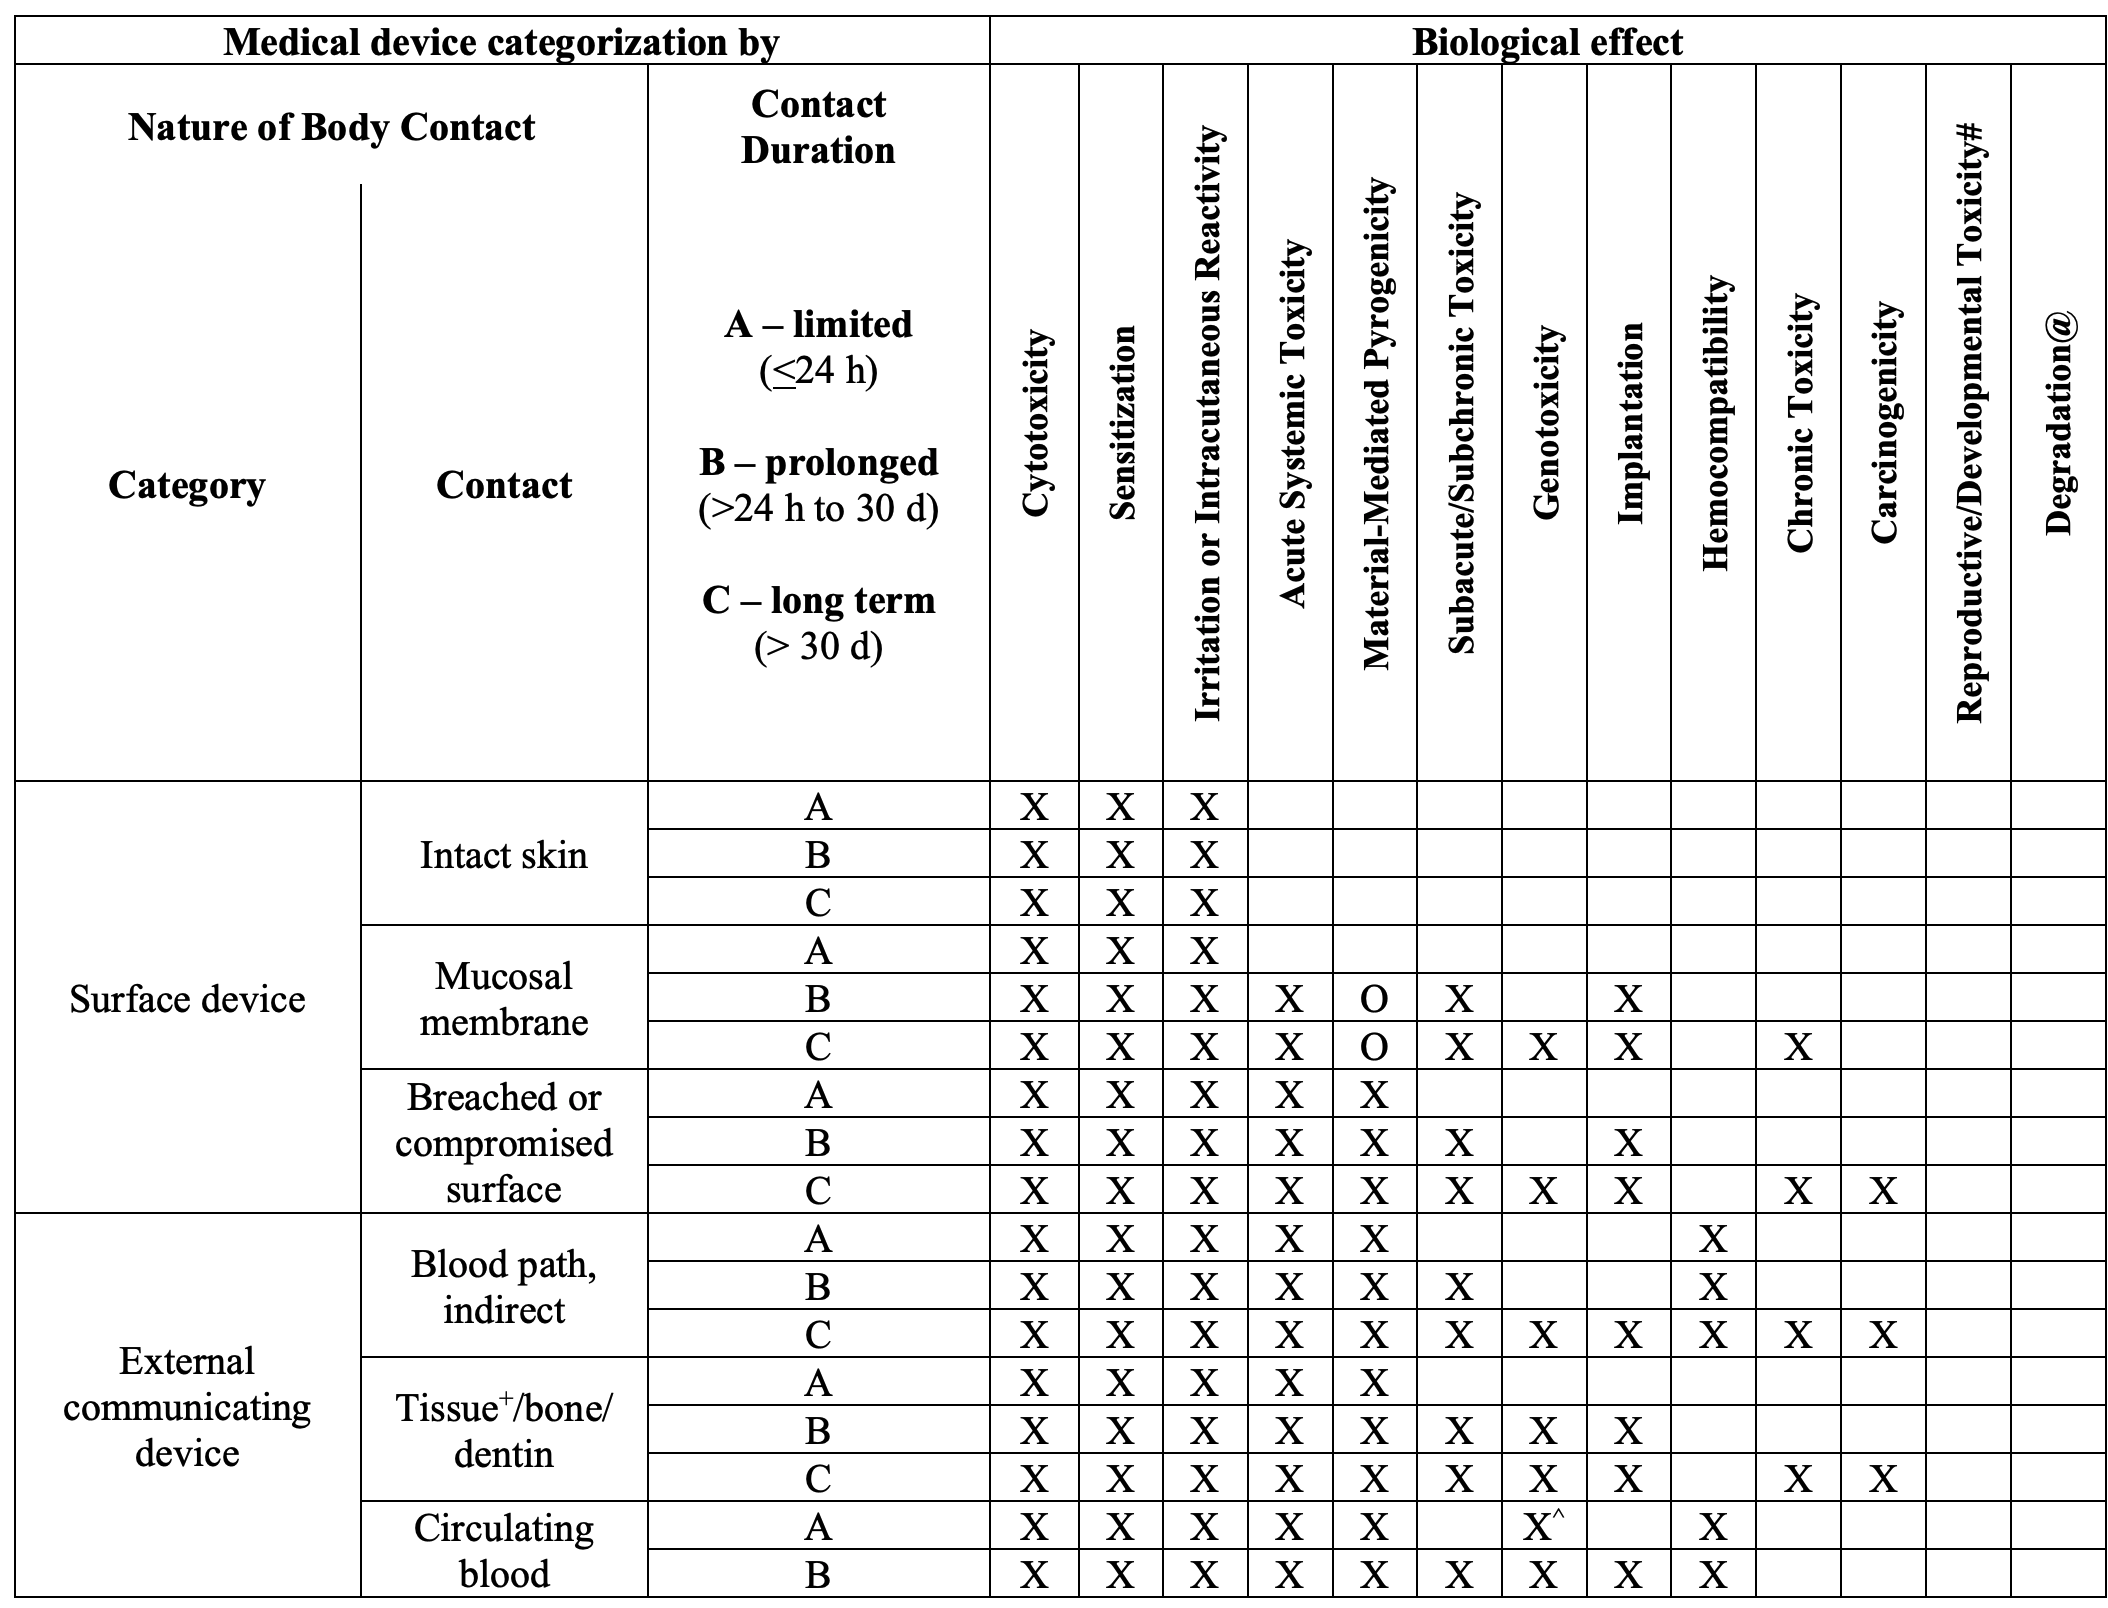
\includegraphics[scale=0.3]{tab1_fda.png}
	\centering
\end{figure}

Figure 3: Table A part 1 in FDA guidance \cite{healthUseInternationalStandard2023}, biocompatibility evaluation endpoints.

\begin{figure}[H]

	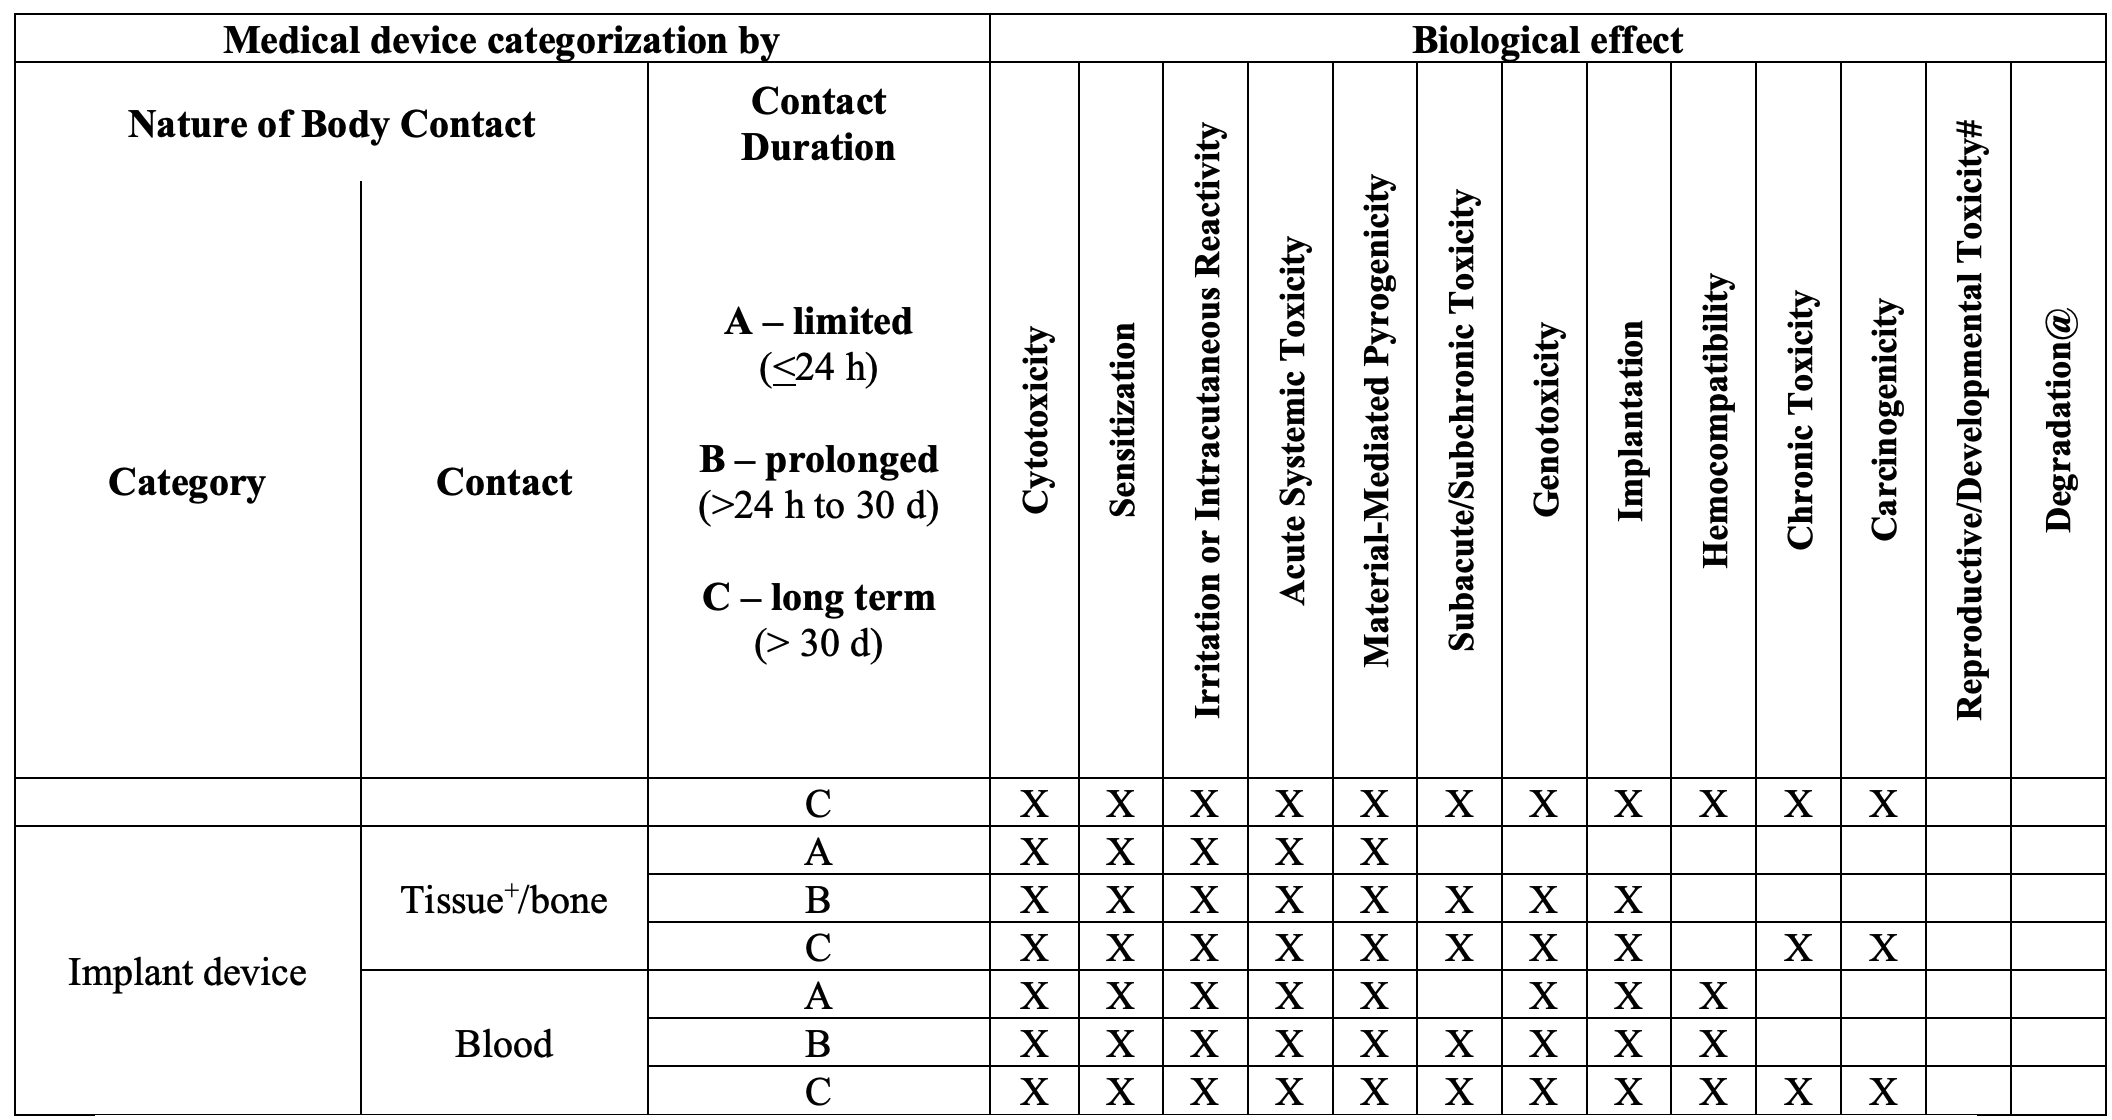
\includegraphics[scale=0.3]{tab2_fda.png}
	\centering
\end{figure}

Figure 4: Table A part 2 in FDA guidance \cite{healthUseInternationalStandard2023}, biocompatibility evaluation endpoints.

The table in Figure 3 and in Figure 4 shows, bases on the category of the product and the tissue and duration of contact, which could the possible biological effect that should be considered for the approval of the specific device.
Senseback could fall into the external communicating device category, with a long-term contact and tissue surface of contact, with relative biological effects reported in the table.  
FDA suggests that this table should not be threated as a checklist for testing. Instead, some specific medical devices the reported effects could not be enough and other endpoints should be considered.
For what concern cytotoxicity, the related ISO standard is 10993-5:2009 \cite{14:00-17:00ISO1099352009a}, a recent study \cite{gruberToxicNotToxic2023} has been conducted in order to verify whether this standard is clear enough to guarantee that devices development which have followed this standard are cytotoxicity safe. The conclusions report that different that this standard should be revised, because cytotoxicity tests performed by different companies with same standard cannot guarantee reliable and comparable results. This standard was last reviewed and confirmed in 2022. Therefore, this version remains current. 
UE regulations
In UE the normative that regulate the medical devices approval are the 2017/745/UE \cite{RegolamentoUE20172017} which is relative to medical devices and 2017/746/UE \cite{RegolamentoUE20172017a}, which is relative to in vitro diagnostic. The first one is applied since 26, May 2021, the second one since 26, May 2022 \cite{MedicalDevicesEuropean}. 
In these regulations, as before, devices are divided into classes of risks from the lowest, which is Class I to Class II-a and Class II-b to Class III, which is the highest one. The device classification follows similar step as in FDA evaluation, in fact some parameters are evaluated such as duration of contact, invasiveness, specific medical purpose and anatomical location \cite{} mcdg , it is up to the manufacturer to correctly classify the device according to the appropriate class of risk.
As reported in the regulations, all implanted medical devices and long-term surgically invasive devices are classified as class IIb \cite{}mcdg . However, since Senseback is an active device, which means that needs a source of energy which is different from the body itself, it could fall into class III, the highest one.
With the new normative UE 2023/607 \cite{RegolamentoUE20232023} the deadline for the manufacturers to adequate to 2017/745/UE and 2017/746/UE has been postponed based on the class of risk of the devices as shown in Figure 5


Figure 5: new date of application of normative (EU) 2017/745 and (EU) 2017/746 according to (EU) 2023/607 \cite{NewRevisedResource}

\subsection{Medical software regulation}

According to the regulations EU 2017/745 \cite{RegolamentoUE20172017} and EU 2017/746 \cite{RegolamentoUE20172017a}, a medical software that is intended to be used alone or in combination with a hardware which fall under the definition of medical device should be considered as a medical device software (MDSW). 
In order to understand whether or not the software could be considered as a MDWS, the steps are reported in.

Figure 6: steps to verify whether or not the software falls into the MDSW definition according to European Commission \cite{} b865

First step is to verify that the software under analysis fall under the definition of software in the regulations, as reported in \cite{} untitled , which states that “software” is defined as a set of instructions that processes input data and creates output data. Second step is to determine whether or not the software influences or drives the hardware device, if it does it could be classified as an accessory for the hardware medical device and as a consequence, be considered as a MDSW. If not, next steps need to verify which is the function for which the software is intended to be used, including whether or not the software provides an effective benefit to the patient. If it does and the software falls under the definition of MDSW in \cite{} untitled, which states that a MDSW is a software that is intended to be used, alone or in combination, for a purpose as specified in the definition of a “medical device” in the medical devices regulation or in vitro diagnostic medical devices regulation, than the software should be treated as a medical device and it is covered by the new MDR regulations.
To sum up, a software is classified as a medical device if it satisfies the following characteristics: it should be independent, so it should have its own medical purpose, it can influence or drive the hardware medical device and it may be intended to be used by medical professionals. Note that a software can be classified ad a MDSW no matter the location intended for it.

The rules to classify a MDSW are reported in Annex VII \cite{massimopANNEXVIII2019}. As it is reported in chapter II, a software which is stand alone and has not influence on the hardware medical device should be classified separately. If it is not, however, it should be classified considering the most critical specified use. I the software and the hardware have two different classes of risks, as a consequence, they both fall into the highest class.

Senseback software, then, falls into the class of risk III. 

\subsection{Normatives for wireless devices}

In European Union, normative EU 2017/745 \cite{RegolamentoUE20172017} treat a wide range of medical devices, including the ones with a radio frequency communication such as Bluetooth low energy like the case in analysis. It is reported that manufacturers should ensure that devices are designed in a way so that external interferences such as external environment or radio signal interferences are removed or at least reduced as much as possible, so it is for possible undesired interaction with the environment which is thought for the device to be used with. 
In the United States, instead, FDA has provided a regulation \cite{healthWirelessMedicalDevices2023} which regards specifically radio frequency wireless medical devices, this is thought for all the devices which use at least one functionality with a wireless feature such as Bluetooth, WI-FI and so on. 
In this normative it is reported that wireless communication could be a benefit for the patient in terms of mobility, due to the fact that wires are not present anymore, moreover also a remote monitoring of the real-time health of the patient is possible. However, possible risks in patient daily life should be considered, and it is up to the manufacturer to inform the patient about them. Firstly, a possible issue regards the fact that airways are shared, and the device could be influenced by other devices operating the near range of work of the medical device which is intended to be used. The increasing usage of these kinds of products, including the non-medical one, could condition the medical device performance. The suggested aspects that the manufacturer should take into consideration are the following ones then:
Selection of the wireless technology 
\begin{itemize}

	\item Quality of service
	\item  Coexistence
	\item  Security
	\item  Electromagnetic Compatibility (EMC)

\end{itemize}
For these, many standards are directly suggested by FDA itself, such as the directives AAMI TIR 69 \cite{RecognizedConsensusStandards} or ANSI C63-27/D1.0 \cite{IEEEANSIC63} for what concern the Wireless coexistence or IEC 60601-1-2 \cite{IEC60601122014} for electromagnetic compatibility (EMC).
For the security field FDA issued a guidance \cite{healthCybersecurityMedicalDevices2023} on September 2023 which regards specifically the cybersecurity in Medical devices, this document substitute the previous one \cite{ContentPremarketSubmissions} issued on October 2014.


\subsection{FDA Medical devices cybersecurity }


According to FDA guidance \cite{healthCybersecurityMedicalDevices2023}, manufacturers have the responsibility of the identification of possible cybersecurity risks associated to their devices, including both the ones related to the device itself and the ones related to the environment in which the product operates, for example the ones introduced by device reliance on hospital networks.
FDA also recommends the submitting of a detailed documentation about the security features of the product which is intended to be approved by them. They also recommend that this information should take the form of views in order to effectively prove that the developed architectures are effective and safe. Manufacturers should demonstrate that security features are effectively been implemented and tested.
The necessary requirements asked by FDA are the following ones:
\begin{itemize}
	\item Authentication
	\item Authorization
	\item Cryptography 
	\item Code, Data and Execution Integrity
	\item Confidentiality
	\item Event Detection and Logging
	\item Resiliency and recovery
	\item Updatability and Patchability
\end{itemize}
Note that these aspects are just the suggested ones, but the necessary features may vary depending on the specific intended usage of the device.
These aspects are explained in detail in Appendix 1
\subsubsection{Authentication}
Authentication is divided into two controls: 
\begin{itemize}
	\item Authentication of information: this means that it is possible to prove that data are generated from a trusted and verified source and they have not been altered during the transmission to the endpoint.
	\item Authentication of entities: it is possible to prove the identity of an endpoint from which is the one which provides information.
\end{itemize}
The device then, needs to verify that information received from an external source are reliable and so are the ones generated from the device itself. 
Authenticity can then be evaluated for:
\begin{itemize}
	\item Information at rest (stored)
	\item Information in transit (transmitted)
	\item Entity authentication of communication endpoints 
	\item Software binaries
	\item Integrity of the execution state of currently running software 
	\item Any other appropriate parts of the medical device system where manufacturer’s threat model and/or risk analyses reveal the need for it
\end{itemize}
The effective strength of the authentication implemented is evaluated on the difficulty that an external unauthorised source would need to identify the decomposition of authentication scheme.
A cryptographic algorithm in general should be preferred, this is because non-cryptographic ones are generally weak. As a consequence, an attacker could easily emulate the behaviour of an authorized user.
Some of the other recommendations regards the usage of a proper authentication method such as the multi-factors ones, strong passwords choices, authentication requirement before possible software updates, anti-replay measure in communications which can result harmful and the avoidance of cyclic redundant checks as security control.
Furthermore, manufacturer should consider how the device reacts to a possible authentication failure.  
\subsubsection{Authorization} 
Authorization is required in order to prevent the access to sensitive information or resources. In a well-designed system, only an authorized which has fully permissions can have the access to specific functions of the medical device, depending of the least privilege principle. This means that, in case of a hacker attack, they should not be able to access to possible functionality reserved to the manufacturer in case they gained the credential associated to patient privilege.
The recommendation about authorization regards the access to the device, which should be limited to authorized users, the usage of timer in order to terminate sessions and “deny by default” principle, which means that device should reject unauthorized connections by default.
\subsubsection{Cryptography} 
About cryptography, this is suggested to be implemented because of its higher level of security. It is underlined that this should be properly implemented to avoid undesired vulnerabilities.
The recommendation which regards this field suggest the usage of industry-standard cryptographic algorithms, in particular the one suggested in the current NIST standard for cryptography, the algorithm should also allow the device to use the highest level of security possible, unless otherwise necessary. Recommendation also suggests avoiding a situation in which the fully revealing of the key for a specific device could implicate the revealing of keys for other devices. Eventually, it is suggested avoiding downgrades in security level unless they are strictly necessary for the health of the patient.
\subsubsection{Code, Data and Execution Integrity } 
Integrity is subdivided into three field: Code, Data and Execution. 
In the code field it is suggested, in addition to previous suggestions, to prefer, when possible, solution which are hardware-based, to disable the access to unauthorized ports such as the UART and to ensure that device is physically integer by employing the usage of tamper seals.
For data integrity, the suggestions regard the verification of the received data coming from an external source, which should be validated and not modified during the transit and the protection of the data which are relevant for the safeness of the device. 
Finally, for the execution integrity purposes it is suggested to use industry-accepted best practices to maintain the code integrity during the execution process and the design and review all code that handles external data.

\subsubsection{Confidentiality} 

Even if authentication ad authorization suggestions provided in previous points should be enough to ensure confidentiality, manufacturers should verify if for the specific implementation it could be necessary to implement additional features. A loss of confidential could result in a potential harmful effect on the patient.
\subsubsection{Event detection and logging} 
The suggestions regarding this point suggest that each security relevant event, in particular suspicious behaviours should be detected and logged promptly, including possible software changes or malfunctions. Manufacturers should also implement a log file in which these tracked events are stored. It is also suggested to design devices which are able to integrate antivirus/anti-malware protections.
\subsubsection{Resiliency and recovery} 
Resiliency and recovery are the capabilities of the device to face with a safety margin a possible incident scenario and maintain availability.
Manufacturers should then design devices which are resilient to possible incidents or noises, specifying the level of resilience that any component of the medical device have. Th design should also include methods for recovery default configurations and protections for critical functionality or data.
\subsubsection{Firmware and software updates} 
Last recommendations regard software and firmware updates. These should anticipate the future cybersecurity vulnerabilities, should be reliable even in case of interruption or failure of the process, and the cybersecurity related ones should be separated from regular feature update cycles. 
Moreover, it is indicated that updates should be easily verified, validated and distributed. Manufacturers should also implement all the necessary tools and processes to ensure that updates are applied in a safely ad timely manner. Lastly, third party licenses should be maintained for the whole life of the device.
\subsubsection{Cybersecurity regulations for medical devices in EU} 
Regarding cybersecurity, the European Union has recently issued the (EU) 2022/2555 \cite{DirectiveEU20222022} normative on Security of Networks and Information systems (NIS2), which is entered into force in January 2023. 
The normative is not just focused on medical device as the FDA guidance \cite{ContentPremarketSubmissions}, but it also discusses about them. The first article reports that the purpose of this normative is to establish rules in terms of cybersecurity risk management for the topics which are considered “critical” in normative 2022/2557 \cite{} publicationsoffice or the ones reported in the Annex I or Annex II of (EU) 2022/2555, such as point 5.a of Annex II which is referred to the fabrication of medical devices and diagnostic medical devices in vitro. 
In NIS2 a distinction had been made between important entities and essential ones, allowing to have in this way a fair trade-off between risks-based requirements and relative obligations and administrative burden stemming. As it is reported in Article 3, entities in Annex II could be classified as essential depending on whether or not they are classified like that by a Member State.
One of the main differences in terms of regulations between important entities and essential entities is the fact that the essential ones are proactively supervised by the authorities, while important ones are subject just to a light ex post supervisory regime, which can be triggered in cases in which evidence of a possible infringement of the directives are brought to the authorities.
In the article 21 point 2 of the NIS2 directive cybersecurity management measures are threated, which both essential and important entities should follow. It is reported that companies have to manage their own security risks and take adequate measures to manage them. 
The recommendations about the measures to take are reported below. They need to include:
\begin{itemize}
	\item Policies on risk analysis and information system security 
	\item Incident handling
	\item Business continuity and crisis management
	\item Supply chain security
	\item Security in network and system acquisition
	\item Policies and procedures to assess the effectiveness of cybersecurity risk management measures
	\item Cryptography and encryption, and multi-factor authentication
	\item Cybersecurity training and basic cyber hygiene practices
\end{itemize}



\section{Ethical concerns}

Even if scientific and biomedical research is essential for the development of our society, it helps people to recover from medical diseases which were chronical before for example, it is important to wonder which is the limit that medical research should reach.
Ethical implications should then be considered, especially in some setups like the one considered in this Master Thesis, which purpose is to have in close future an effective usage in vivo.
In all of the steps, from the premarket ones and relative experimentations to the post market ones and relative surveillance, ethic should be taken as a monitor, in order to guarantee that not only the device in use is safe and effective, but also the development of it has been made respecting environment, the work ethic of people involved in, and the eventual animals used for the experimentation phase. To do that, research should be the as transparent as possible, by clearly explaining the goals and the intended benefits of the project, the methods and design of the study and which could be the possible risks. 
When available the results of the study should be published, possibly even the experimental ones. This would contribute to the check of the results by other researchers, promoting the re-doability and consenting a critical evaluation of the work. In case of possible criticisms or questions coming from the scientific community, these should be answered, and corrective actions should be taken when necessary. The practicality of sharing the information on the project is essential in an ethical and responsible research. 
Some of the principal ethical topics that should be considered are treated in detail below.


\subsection{Animal welfare }

The first aspect that should be considered for this purpose is animal welfare. The World Organisation for Animal Health (OIE), defined animal welfare as follows: An animal is in a good state of welfare, if it is healthy, comfortable, well-nourished, safe, able to express innate behaviour, and if it is not suffering from unpleasant states such as pain, fear and distress \cite{Chapter}. Animal welfare, in this kind of research, implies the careful and responsible consideration of the management, the treatment and health conditions of the animals involved in the research.
Animals are still necessary to test pharmaceutical or medical products before putting them into the market, because the experimental phase made on animals guarantees that each product on the market is effectively safe and which could be eventual collateral effects that patients should be warned about. However, the treatment of the animals involved in the experiments must be ethically correct. This means that this phase should respect current rules and animal welfare regulations, and this also means that animal experimentation is made only when necessary and the least number of animals is involved. 
The Animal Welfare Act (AWA) \cite{}comps was the first policy responsible for guaranteeing the standards for animal welfare in the USA. It included rules relative to transportation, treatment during tests and research, teaching and dealings by animal dealers. This standard was issued in 1966, but it only covered some warm-blooded animals such as dogs, cats or rabbits, and some other animals like birds or rats, which are the ones mostly used in scientific experiments, were excluded from the act. The Act was amended eight times until now, however it is just in 2002 with the publication of Farm Security and Rural Investment Act \cite{}plaw that the excluded animals, including rats used in medical research, has been included into the definition of “animals” of the Animal Welfare Act.
The European Union also issued some policies to define the minimum standards necessary for animal welfare, which are some of the world’s highest animal welfare standards \cite{AnimalWelfareEU}. The current normative responsible for setting this kind of standards in the EU is the 2010/63/EU \cite{Direttiva201063}, published in 2010 and effective 1 January 2013. It is strictly related to animals used for scientific research and treats all the related steps, from development to manufacture to tests. The ultimate goal would be to have fully non-animal methods.
By following these policies and by implementing the right measurements to guarantee animals well-being, it is possible to reduce the negative impact on the life of the animals involved in the study.
Some of the terms that implies a sufficient welfare of the animal are:
Implant procedure. The chirurgical procedure necessary for the implanting of the device should be painless and as less invasive as possible. It is important to reduce at the minimum the pain of the patient during this operation and guarantee that the patient would have sufficient time for recovery after that. 
Health monitoring. The health of the patient should be monitored for the whole time of the experiment. This includes the monitoring of vital functions, the behaviour of the animal and physiologic indicators.
Duration of the experiment. The experiment duration should have the strictly necessary duration to get the necessary data for the experiment. The minimum number possible of involved animals should also be considered.
Usage of positive and negative controls. They should be implemented in order to check if the observed effects are due to the intervention or external environment.
Environment in which animals live. This should guarantee that animals' physiological needs are respected. These include water and food access other than movement range and social iteration.
Biological behaviour of the animals. The natural behaviour of the animal involved in the experiment should be respected, including the possible negative impacts on their daily life, which should be minimised.
In those cases in which euthanasia is necessary, it should be performed in agreement with the current normative of the corresponding country. This process should be conducted in a way which is ethical and respectful towards animals, making sure that this is conducted with attention on animal welfare. 
When possible, animal usage should be avoided in favour of cultured cells and computer-based models.
Transparency. The documentation of all the precautions taken during the study underlines the ethical diligence of the research.





\subsection{Need of research}


When approaching biomedical research, in which living beings are involved, it should be considered whether or not the intended research is necessary and whether or not the purpose of the research could be reached without animal usage. It is important for this purpose to make a trade-off between the possible benefits that people or animals could get from the research and the eventual damages caused to animals. 
The concept of “Need” for research refers to whether or not there is proper justification and needs to conduct the intended research. This means that developers should wonder whether or not the research faces a significant demand in the scientific development and in practical applications, these could justify resources usage and experimentations conducted on the animals.
In order to make sure that ethical implications have correctly been monitored in the intended experiment, it is suggested to submit it to a careful revision from an ethical committee or institutional ones. 
To sum up, needs of the research means carefully wondering about the scientific and ethical value of the project, making sure that these justify animal involvement. These precautions make sure that research is conducted in a responsible way and it is in line with the highest ethical standards.

\subsection{Safety of the patient}


The concept of safety of the patient is fundamental for guaranteeing that the iteration between the device implanted in the animal’s body and the external device happens in a safe way and it does not involve any risks for the animal's health.
One of the first aspects that should be considered for this purpose, is the fact that materials should be safe and biocompatible. The utilised components should minimise risks and adverse reactions in surrounding tissues. A careful planning and a correct post-operation management could contribute to reducing the minimum uneasiness and collateral effects.
Moreover, during the implantation procedure, protocols should be adopted in order to prevent possible risks of infections. Hygiene is essential to prevent issues that could intact the safety of the animal.
Furthermore, considering that Senseback communicates with the external device wirelessly, the right procedures for assuring that the protocol of communication, in this case for Bluetooth Low Energy (BLE), is secure and cryptographed in order to protect sensitive data. This is essential for the protection of the privacy of the patient.
Lastly, it is important to consider the procedure to follow in those cases in which the experiment presents issues or complications. This includes the planning of emergency procedures and the possibility to interrupt the experiment if some warnings related to the safety of the patient come up.

\subsection{Inclusivity}
 

The concepts of inclusivity and heterogeneity are linked to ethical and social considerations related to equal access, representation and to the individual differences in the process of research and in the application of the results.
Firstly, the project should promote equality in the access of the benefits coming from the research. This includes the consideration on how the application of the technology can be made available to different ethnic groups, avoiding discriminations and differences in the therapeutic approach.
Talking about this specific project, this is intended to be experimented on animals in next few years, however in a distant future this should be made available on humans. For this reason, the differences between the group of patients should be taken into consideration, to make the project more general and inclusive. An example of this is a study, \cite{nagaokaDevelopmentRealisticHighresolution2004} proposed by Institute of Physic and Engineering in Medicine (IPEM), in which a whole-body voxel model for the average Japanese man and woman has been developed. This study shows how different are some physical effects such as SAR on the body. A comparison with previous studies, in which only Caucasian men were studied, has been performed in order to underline the differences. This study should be taken as a monitor to take into account that different bodies of men and women of different ethnicities could have some substantial differences. Moreover, the project should also respect individual differences in response to technology in order to maximise efficiency and minimise collateral effect. Some genetic, physiologic or lifestyle related variations or possible disabilities can influence the response of the patient to the treatment. The project should then be relatable for the higher range of individuals possible, including the ones with special needs. Furthermore, the manufacturer should also consider how the related project could impact society in terms of inclusion and diversity and which could be possible positive or negative effects on social dynamics and equity of health.
Inclusivity could also mean the respect for different cultural sensitivities, which should be taken into account in the design of the project. Medical practices could vary by varying the country and these differences must be considered. Research could work in strict contact with the related community, this could help to better understand the needs and the expectation of the people involved.
Also the informed agreement in case of experimentation on humans should be sensitive to culture and should be understandable for all the participants. Information contained in that should respect differences in terms of language and culture.
All in all, the concepts of inclusivity and diversity focused on the obtaining of an equal approach, representative and respectful of the differences both in the research phase and in the usage one. The attention to these considerations would contribute to guarantee that the project has a positive impact on a larger range of individuals and communities.


\subsection{Informed agreement }

Informed agreement is crucial in those projects in which humans are involved in experimental research or in the application of new medical technologies. The informed agreement is an ethical process which guarantees that all the participants have a complete view of the intended purposes, the risks and the possible benefits of the research or the medical intervention in which they have given their voluntary consent to participate. Before submitting anyone to experimental treatments or to procedures linked to the related technology, it is necessary to get an informed agreement.
In the agreement it is important to furnish to the participants all the necessary details about the procedure, including the goals of the study, the kind of intervention that will be made and possible issues or risks. All of the available options should be illustrated, and information about possible alternative or standard treatments. This allows participants to make clear decisions about their participation. 
The agreement should also assure that anyone who is not purported to participate anymore could retire themselves from the study without any negative consequence. This enforces the principle of voluntary consent and respect about the autonomous decision of the participant.
The operator should explain in detail and in a clear manner how technology will work in the context of treatment or research. The participants should have the chance to ask questions and receive clarifications about the utilised technology.
For what concerns animals, since they cannot give a proper informed agreement, it becomes more and more important to have a consent from an ethical committee and from authorities. This will assure that animal welfare is respected.
Ultimately, researchers should have a clear documentation of the informed agreement, including the details related to the explanation given, the comprehension from the participants and their signs. This documentation is fundamental for transparency and ethical conformity.
To conclude, assuring that an informed agreement is obtained in a complete and ethical manner is fundamental for the respect of rights and dignity of the human or animals participants involved in the project.

\subsection{Privacy and surveillance}


Considering that in the Senseback project a wireless communication (BLE) is used, the concepts of surveillance and privacy are fundamentals and should be treated.
It is essential that, in the communication, security regarding the transmission of data is guaranteed. To do that, all the necessary robust precautions, such as cryptography, should be taken, in order to protect the communications from possible non authorised interceptions. It is also important to focus on the nature of the transmitted data, only necessary information should be shared, and the communication should be limited to the finalities related to the project.
Due to the sensitive nature of the biological or medical information, the privacy of the generated data should also be protected. To do that, measures to guarantee that data are treated in accordance with privacy-related laws and ethical standards becomes crucial. Moreover, collected data should be conserved and stored in a secure way, by limiting the access just to necessary cases and by implementing security protocols to avoid losses, manipulations and unauthorised accesses.
Another precautions to guarantee the privacy of the patient is the anonymity of the data when possible, especially in those cases in which data are shared or aggregated. This would protect the identity of the patient involved in the project.
Other than communication, also the device in usage should be securely designed. This includes protections against unauthorised access to the device itself and preventions against possible risks linked to the implant.
In addition, during the informed agreement, human participants should be warned about data management and privacy. They should have a clear explanation about how their personal information will be treated and an explicit agreement about storage and usage of data should be furnished. In particular, it is important to follow the norms related to the privacy of the patient in the related geographical context, in order to guarantee that the project is ethically and legally acceptable. In EU privacy is regulated by the General Data Protection Regulation (GDPR) \cite{L_2016119EN01000101Xml}, whose publication has provided a clear regulation for personal data treatment. In the USA, privacy regulation is not uniform and it is present just in some states like in California with the California Consumer Privacy Act (CCPA) \cite{}california or in Virginia with the Virginia Consumer Data Protection Act (VCDP) \cite{CodeVirginiaCode}. Normative however, should be continuously monitored, since dynamics related to privacy can evolve and the adaptation to new normative or to the recent ethical worries is essential.
To sum up, the concepts of surveillance and privacy regard the responsible management of sensitive information, while it is guaranteed that secure measurements are in line with the ethical and legal normative applicable. This is fundamental to respect the rights and dignity of the involved people and to maintain trust in the research. 



\section{Signal Acquisition}



\chapter{State of the Art}



\section{Introduction to Bluetooth Low Energy}

Firstly, we need to define that "Bluetooth low energy is a brand new technology that has been designed as both a complementary
technology to classic Bluetooth as well as the lowest possible power wireless technology that can be
designed and built. Although it uses the Bluetooth brand and borrows a lot of technology from its
parent, Bluetooth low energy should be considered a different technology, addressing different design
goals". \cite{heydonBluetoothLowEnergy2015}
""chiara""
The main advantage of the BLE over the
standard Bluetooth is that it keeps the radio off as much as possible when no data has
to be sent [47]. It is optimized for low power consumption and short-range
communication; thus, it enables devices to operate on a small energy budget, making
Bluetooth technology is based on a master-slave concept, where one device acts as the
master and controls one or more slave devices. The master initiates and maintains the
communication, while the slave devices respond to the master's commands. For this
there are four roles that a BLE device can implement. A device can be a peripheral
(slave), it advertises their presence and respond to central devices' requests. A central
(master), instead, scans for these advertising packets and it could, if the advertisement
packet allows it, connect to that device. Moreover, there are other two roles possible:
the broadcaster and the observer. A broadcaster sends out advertising packets without
allowing any connections, while an observer discovers peripherals and broadcasters,
but without the capability of accepting connections from a central.
""chiara""

\section{Communication system}
\section{Previous code implementation}



As show in the introduction, Senseback is an implanted device which communicates with an external unit through Bluetooth Low Energy. The starting point for the firmware code of this communication was previously developed [Chiara Master Thesis]. This master thesis purposes improvement and additional features on the previous code, which presents some limitations.

\begin{figure}[H]
	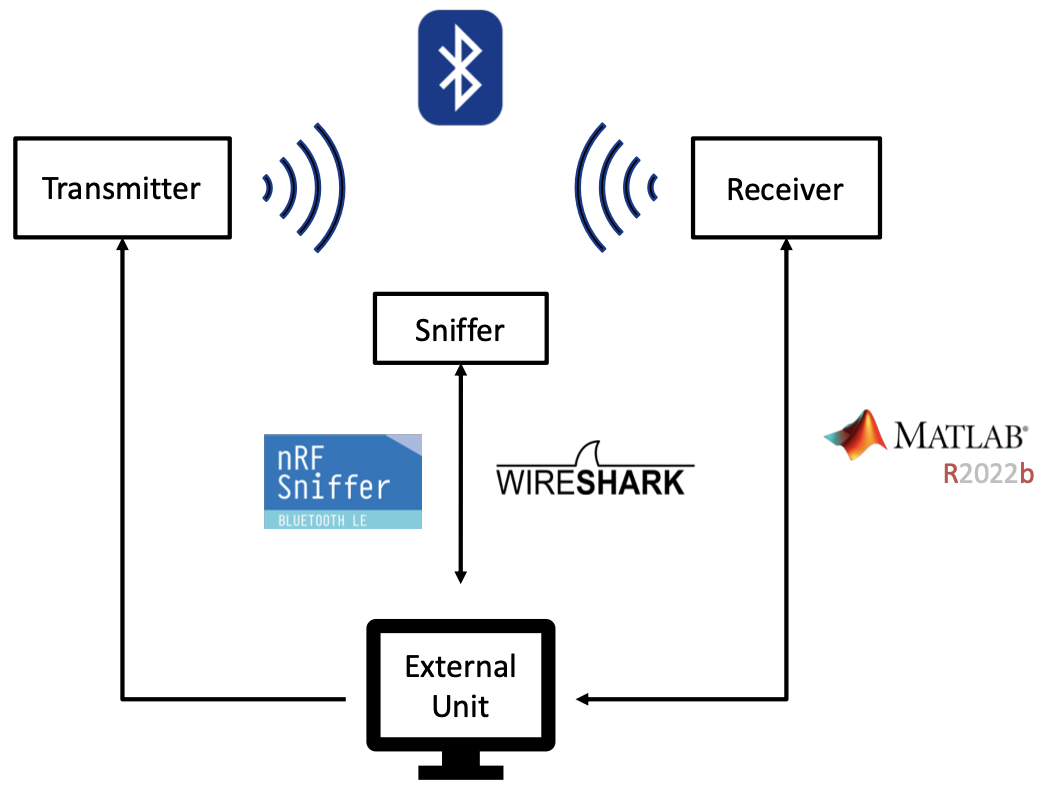
\includegraphics[scale=0.3]{prev1.png.png}
	\centering
\end{figure}

Figure 1: BLE communication between Senseback and external device
The general architecture for the previous code is shown in Figure 2.

\begin{figure}[H]
	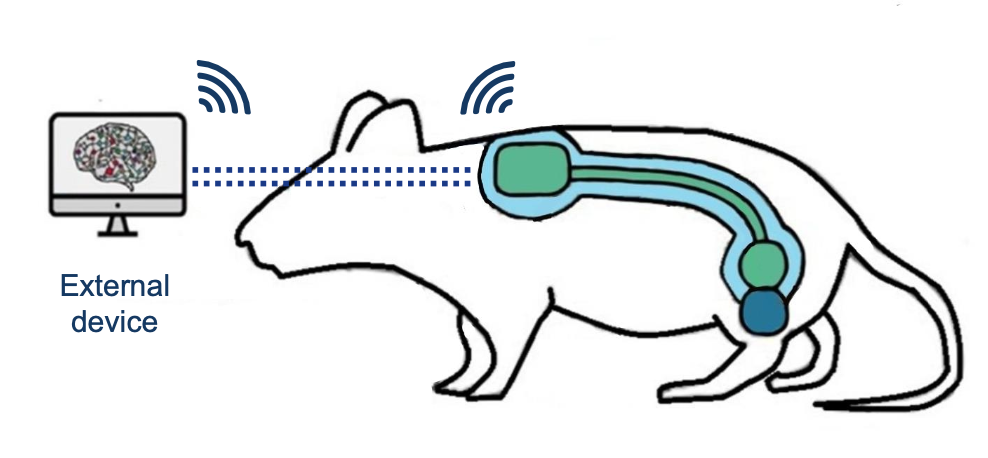
\includegraphics[scale=0.3]{prev2.png.png}
	\centering
\end{figure}



Figure 2: Previous implementation, setup of the experiment.
As is it possible to see, two main devices facilitate communication: the transmitter and the receiver. For the experiment, two identical nRF52 Development Kits (DKs) \cite{NRF52DKDevelopment} were used as the transmitter and receiver. These boards were thought to be employed just for testing, the final implementation, in fact, will replace the transmitter board with the Senseback device, and the external unit will serve as the receiver. Both boards were powered and controlled through the external unit, which was a PC connected via serial ports.
External unit allowed the user to manage the communication by sending "START," "STOP," and "RESET" commands. This was done thanks to the usage of a Matlab script. These commands were transmitted through the serial port and received by the receiver using Universal Asynchronous Receiver/Transmitter (UART). UART is a common serial communication protocol used for connecting microcontrollers and other devices, often facilitated by USB-UART converters \cite{LessonSerialCommunication}.
For both the transmitter and receiver, separate codes were implemented to manage communication. The first code set, designated as "Offline," was designed to test communication with a fixed number of packets. Specifically, 32,400 packets of one byte each were transmitted. The test began when the user entered the "START{\textbackslash}n" command through MATLAB, giving the signal to the transmitter to start sending packets. This test ended when all packets were sent. The "Online" communication, on the other hand, simulated real-time behaviour with no predefined packet count. This test also begun once the user digited the "START{\textbackslash}n" command, but it required also a "STOP{\textbackslash}n" command to end. Lastly, the "RESET{\textbackslash}n" command was just used in those cases in which it was necessary to restart the communication from the beginning.
Upon receiving the appropriate command in MATLAB, the external unit would send it to the receiver via UART, which then relayed the command to the transmitter through BLE. The transmitter would start sending data to the receiver upon receiving the "START{\textbackslash}n" command and stop when it received the "STOP{\textbackslash}n" command or all packets had been sent, depending on the test mode. After receiving the packets, the receiver printed the data to the serial port, allowing the external unit to read it through MATLAB. 
Last element of the previous setup is the sniffer. The purpose of this was to detect the packets exchanged from transmitter and receiver, including possible retransmissions during the communication. The chosen software to play this role is Wireshark (v.4.0.6) with the nRF Sniffer Tool (v.4.1.1), provided by Nordic Semiconductor©.
All the codes used for this setup are deeply analysed below.

\subsection{Matlab scripts}

To achieve the two main objectives of communication control and data verification through a serial port, two separate MATLAB scripts were created. The first script is designed for offline testing, the second one for online. Here's how they work:
Both scripts start by creating a vector that simulates the incoming ADC samples from a Senseback device. These samples are in uint16 format. Each value is then split into two uint8 values using the MATLAB function typecast, ensuring that the data is converted without losing information. The next step is to set up the serial port with a baud rate of 115200 bps, whose limit is imposed by the UART communication. After setting the baud rate, the serial port is flushed to ensure it's clear before communication begins.
The scripts, instead, differ in the following ways:
Commands: In the offline test script, only one command is required from the user, while the online test script requires two commands, the start and the stop of the communication.
Data Reception: The online script does not include any data reception functionality due to memory limitations and the slower baud rate. In contrast, the offline script does receive data from the serial port.
The online test script is simpler, focusing on generating the data and ensuring the serial port is set up properly. There is no data reception because of the limitations mentioned earlier.
The offline test script uses a callback function to handle data reception. It uses the MATLAB configureCallback function to call the readData function each time new data is received from the selected serial port. The purpose of this function is to store the incoming data in a vector and keep track of the total data received. The callback function is turned off when the last two values are both 255 (indicating the end of a data sequence). Once all data is received, it can be converted back to uint16 using typecast and organized into a matrix for plotting and further analysis. The offline test script can then compare the received data with the data originally generated in MATLAB to ensure its accuracy and reliability.

\subsection{Offline transmitter code}
Figure 3 illustrates a flow chart of the offline code for the transmitter. Each block represents a distinct function. Below is a brief explanation of each one.
Log init: This function initializes the log module. This module provides logging capabilities for the intended embedded application \cite{NordicSemiconductorInfocentera}. It has different usages such as debugging, which means to provide diagnosis for possible issues, info, which implies to check whether or not the application works as expected, warning, so indications about something unexpected which is happened, and error in those cases in which the software is not able to execute one of the functions.
This function initializes the timers. For the offline code of the transmitter, two timers have been used. The first one is the timer responsible for data generation, and the second one is responsible for monitoring the total time required for data generation, data pre-processing, and sending to the central device. The two timers are both equally initialized, with the frequency set to 2 MHz for both.

The main difference between these two timers is given by the functions \texttt{nrfx\_timer\_us\_to\_ticks} and \texttt{nrfx\_timer\_ms\_to\_ticks} for the first and the second timer, respectively. These functions create an interrupt each time the timer reaches the specified value, which is 12.5 $\mu$s for the first one and 1 ms for the second. The value of 12.5 $\mu$s has been chosen to simulate the arrival of samples coming from the ADC in the actual application; in fact, 12.5 $\mu$s represents a frequency of data generation of 80 kHz.

This function is responsible for data generation. Firstly, it checks whether the transmission is active, i.e., whether the command \texttt{START} has been received from the central device. If it is active, a new data \texttt{CNT} is generated. Data generation is done as a step, so each new value is equal to the previous one plus one. \texttt{CNT} is a \texttt{uint16\_t} variable. This choice is made because the ADC samples have 10 bits size, and the \texttt{uint16\_t} variables are the smallest ones which guarantee that the samples are saved without wasting information, which would occur if a \texttt{uint8\_t} variable were chosen.

Once the new \texttt{uint16\_t} data is generated, it is put into the ring buffer \texttt{uartRx}. \texttt{Ringbuf} is a data structure that uses a single, fixed-size buffer as if it were connected end-to-end. This structure is useful for buffering data streams, where data needs to be overwritten as new data comes in, particularly when the buffer is full. It's commonly used in scenarios where the producer and consumer operate at different rates, as in this case. The size of \texttt{uartRx} has been set to 16384 \texttt{uint16\_t} variables, representing the maximum size imposed by the RAM storage limits.

Once \texttt{CNT} has been put into the ring buffer, the function \texttt{data\_arrived}, which is responsible for counting the number of data generated, is incremented by one. Then, it is checked whether the new value generated is the first one using the boolean variable \texttt{first}. If this is still true, as initialized, it means that the new data generated is the first one, so \texttt{timer2} starts counting from a time elapsed equal to zero milliseconds. When the condition \texttt{first=true} is triggered, the boolean variable \texttt{first} is set to \texttt{false}, thus avoiding entering the previous condition in the next cycle and starting \texttt{timer2} again.

The last step for this function is to check whether the data generation process has arrived at the end. This is done by checking the value that the variable \texttt{data\_arrived} has reached. If this value is greater than the value imposed by \(\left(\frac{\texttt{DATA\_TO\_SEND} - 2}{2}\right) - 1\), the condition is triggered. For the offline test, the \texttt{DATA\_TO\_SEND} variable is equal to 32400 and represents the number of bytes that should be sent to the central device to complete an offline test. Consequently, the condition is triggered when the variable \texttt{data\_arrived} has reached a value of 16198, which also represents the number of samples arrived from the ADC. The choice for this condition triggering will be explained in detail when discussing the \texttt{spibuff} process function, which is responsible for data preprocessing before sending.

Once the condition is triggered, the \texttt{data\_arrived}, \texttt{first}, and \texttt{CNT} values are reset, and the last 16-bit value is put into the ring buffer: 65535. This value represents the highest value in binary that can be represented using 16 bits. It is, in fact, a sequence of 16 bits all set to 1. Then, the boolean variable \texttt{transmission} is set to \texttt{false}, indicating that data generation is finished.

Timer2 handler:
\texttt{Timer2} is the timer responsible for the computation of the total time elapsed during the data generation, data preprocessing, and data sending processes. This function increments the variable \texttt{total\_time\_elapsed\_ms} by one each time the interrupt is triggered, so each millisecond. In this way, \texttt{total\_time\_elapsed\_ms} provides a timestamp of the current total time elapsed in milliseconds.


Power management init: this function initializes the power management module, which handles power management features. \cite{NordicSemiconductorInfocenterb}
Ble stack init: This function is responsible for the initialization of the SoftDevice and BLE event interrupts. A SoftDevice is a precompiled and linked binary software implementing a wireless protocol developed by Nordic Semiconductor. \cite{NordicSemiconductorInfocenterc} In this function, it is first requested to enable the SoftDevice using the \texttt{Nrf\_sdh\_enable\_request} function. Once the SoftDevice has been enabled, it is configured through the function \texttt{Nrf\_sdh\_ble\_default\_cfg\_set} by using the default settings specified in the SoftDevice handler BLE configuration. Finally, the functions \texttt{Nrf\_sdh\_ble\_enable} and \texttt{Nrf\_sdh\_ble\_observer} respectively enable the BLE stack and register a handler for BLE events.

Ble evt handler: This function manages the different BLE events. It first creates a pointer to the specific GAP events, then a switch gives the instructions for each different event.

\begin{itemize}
    \item \textbf{First case:} the device is connected. If this case is triggered, a log and the usage of LEDs, enabled through the function \texttt{bsp\_indication\_set}, indicate to the user that the connection has been correctly performed. The connection handle is then stored in the variable \texttt{m\_conn\_handle}. The connection handle is a value provided by the BLE stack that uniquely identifies a connection with another BLE device \cite{BluetoothLowEnergy2016}. Then, the function \texttt{nrf\_ble\_qwr\_conn\_handle\_assign} assigns a connection handle to the given instance of the Queued Writes module \cite{NordicSemiconductorInfocenterd}. Ultimately, the data rate (PHY) is set to 2 Mbps for both the TX and RX BLE characteristics.
    
    \item \textbf{Second case:} the device is disconnected. In this case, it is logged to the user that a disconnection occurred, and the connection handle is set to invalid.
    
    \item \textbf{Third case:} PHY update request. In this case, the data rate is automatically changed to respond to a PHY update request.
    
    \item \textbf{Fourth case:} security parameters request. In this implementation, security features are not implemented, which means that the reply to the security parameters request is that pairing is not supported.
    
    \item \textbf{Fifth case:} system attribute access pending, such as bonding information \cite{NordicSemiconductorInfocenterf}. Again, in this case, no system attribute is stored.
    
    \item \textbf{Next cases:} timeout events. If these are triggered, the connection is terminated.
    
    \item \textbf{Last case:} transmission has been completed. If this happens, the function \texttt{on\_tx\_complete} is called.
\end{itemize}


On Tx complete: This function manages the packet transmission queue mechanism. If the \texttt{BleTxBusy} variable is true, indicating that a packet has not been sent due to the transmission channel being busy, the variable is reset to false. Then, the \texttt{notification\_send} function is called to attempt retransmission. This ensures that no packets are lost, as transmission attempts continue until successful completion.

\section*{Notification Send}
This function oversees the data transmission process and calculates the transmitter's throughput. Initially, a \texttt{uint32\_t} variable \texttt{err\_code} is set to \texttt{NRF\_SUCCESS}, indicating no errors. Before sending data to the receiver, the function checks two conditions:

\begin{itemize}
    \item \textbf{Error Check}: It verifies that \texttt{err\_code} remains \texttt{NRF\_SUCCESS}, ensuring no transmission errors have occurred.
    \item \textbf{Data Availability Check}: It ensures that the \texttt{uint16\_t} variable \texttt{txRdPtr} (index tracking the last number of bytes sent) is less than \texttt{txSize} (total number of available data bytes). This ensures sufficient new data is pre-processed and ready for transmission.
\end{itemize}

If both conditions are satisfied, the length of the new packet to be sent, stored in the \texttt{length} variable, is updated to \texttt{txSize - txRdPtr}. This data of this length is then sent via the \texttt{ble\_nus\_data\_send} function and \texttt{err\_code} is updated accordingly. If \texttt{ble\_nus\_data\_send} completes successfully without errors, \texttt{txRdPtr} is incremented by the size of \texttt{length}, and the \texttt{data\_sent} variable, which tracks the total bytes sent to the central device, is also increased by \texttt{length}. 

Next, the function checks if the transmission has reached the end by verifying if the last two bytes sent are both 255. Since 255 is the maximum value representable with 8 bits, this check ensures the last \texttt{uint16\_t} variable in the ring buffer \texttt{uartRx} (set to 65535 in \texttt{timer1\_handler} function) has been sent. If true, the total elapsed time is calculated by converting the timer ticks of \texttt{timer2} to milliseconds. The throughput is then calculated using the formula: throughput=number of bits senttotal time elapsed
\[
\text{throughput} = \frac{\text{data\_sent} \times 8}{\text{total\_elapsed\_time}}
\]
All relevant values, including the number of waits, are logged. If \texttt{ble\_nus\_data\_send} function returns an error, indicating an unsuccessful transmission, \texttt{bleTxBusy} is set to true, and the wait counter is incremented. Finally, if \texttt{txRdPtr} is greater than or equal to \texttt{txSize}, the \texttt{txActive} variable is set to false, indicating that another packet can be pre-processed.
% Gap params init: this function sets the necessary Generic Access Profile (GAP) parameters of the device, such as security level and the name of the device. In this implementation, since security features have not been implemented, function BLE_GAP_CONN_SEC_MODE_SET_OPEN sets the level of security at the minimum, meaning that the board is totally open. The other parameters that are set in this function are the ones related to the packet exchanges such as minimum and maximum connection interval (CI), the slave latency and the connection superior timeout. These parameters have a great impact on the overall throughput that would be reached in the end.
Gatt init: This function initializes the Generic Attribute Profile (GATT) library. It also sets the Attribute Protocol (ATT) Maximum Transmission Unit (MTU). This parameter defines the maximum amount of data that can be exchanged by a single BLE packet, specifically for the peripheral side. For this application, the MTU has been set to \texttt{NRF\_SDH\_BLE\_GATT\_MAX\_MTU\_SIZE}, which corresponds to a value of 247 bytes, the maximum achievable with BLE version 5.2. A high value for \texttt{GATT\_MTU} generally implies higher efficiency for data exchange and consequently, a higher throughput. In fact, with a single exchange, it is possible to send a larger amount of data, minimizing the wasted time due to latency.

\section*{GATT Event Handler}

This function handles events coming from the GATT library. It first checks whether the event triggering is caused by the current connection by looking at the connection handle stored in the variable \texttt{m\_conn\_handle}. In this implementation, the condition will always be triggered since there is only one connection, which is point-to-point. It also checks, together with the previous condition, whether the event that occurred is an update of the GATT ATT MTU. If both these conditions are satisfied, then the \texttt{m\_ble\_nus\_max\_data\_len} variable is updated to the effective ATT Payload for the connection, which is equal to ATT Data minus the two headers shown in Figure 4, specifically, the Op Code and the Attribute Handle.

% \begin{figure}[h]
%     \centering
%     % \includegraphics[width=\textwidth]{ble_packet_format.png}
%     \caption{BLE packet format (\href{https://novelbits.io/bluetooth-5-speed-maximum-throughput/}{link})}
% \end{figure}

Once this value is updated, the desired values for ATT MTU of the central and peripheral devices are logged to allow the user to check whether they are the same, ensuring that both devices agree on the maximum achievable value.

\section*{Services Initialization}

This function is used to initialize all the services which will be used in the application. For the intended purposes, the services that are initialized are two: Queued Write Module (qwr) and NUS module. The qwr module handles prepare write, execute write, and cancel write commands. It also manages memory requests related to these operations (\href{https://infocenter.nordicsemi.com/index.jsp?topic=%2Fcom.nordic.infocenter.sdk5.v15.0.0%2Fgroup__nrf__ble__qwr.html}{link}). The NUS module is a custom Bluetooth Low Energy (BLE) service designed to emulate a UART (Universal Asynchronous Receiver/Transmitter) over BLE. This allows devices to communicate wirelessly in a manner similar to serial communication over a wired connection (\href{https://infocenter.nordicsemi.com/index.jsp?topic=%2Fcom.nordic.infocenter.sdk5.v15.0.0%2Fgroup__ble__nus__c.html}{link}).

\section*{NUS Data Handler}

% This function manages the start, stop, and reset occurrences of the BLE communication by checking the command received from the central device. The function starts with an \texttt{if} condition, which checks whether a command is received by the peripheral device via NUS. If this is the case, the value of the received string is saved into the variable \texttt{dongle\_command}. Then, the actual value of the string is checked. If the received string through \texttt{ble\_nus} is equal to ``START\n'', this means that the user has sent the command to begin communication. Consequently, the boolean variable \texttt{transmission} is set to \texttt{true}, indicating that transmission should start, \texttt{timer1} is enabled, and \texttt{timer2} is reset. In this way, data generation starts, and it is ensured that the total time elapsed counter starts from 0. If instead, the command received is equal to ``RESET\n'', then the \texttt{CNT} variable is set to 0, meaning that data generation is reset to the beginning. Finally, if the received command is equal to ``STOP\n'', then \texttt{timer1} is disabled. By stopping the data generation, no more data will be available for transmission, and the whole process of data sending will stop.

\section*{NRF QWR Error Handler}

This function handles Queued Write Module (qwr) errors. A pointer to this function will be passed to each service which may need to inform the application about an error.

Advertising init: This function is used to initialize the advertising functionality of the peripheral device. When a BLE device broadcasts its presence, it sends out advertising packets that can include various types of information, such as device name, service UUIDs, manufacturer-specific data, and appearance. For the current application, the advertising packets include the device’s full name but not the appearance data. Appearance data is a predefined value that indicates the type or category of the device. This value is used to give a general idea of the device's functionality without requiring a full connection. It helps other BLE devices and applications quickly identify what kind of device they are encountering. The choice of not including the appearance value in the advertising packets could be made both for privacy reasons and for saving space for other information. Another included parameter in the advertising packets is the advertising flag field, which in this case is set to \texttt{BLE\_GAP\_ADV\_FLAGS\_LE\_ONLY\_LIMITED\_DISC\_MODE}, meaning that the device only supports BLE and not classic Bluetooth, and that the device will be in a discoverable state for a limited time. 

Furthermore, UUIDs should be defined. A UUID is a unique identifier for services offered by the BLE device. The function \texttt{advertising\_init} first computes the number of UUIDs that are present in the \texttt{m\_adv\_uuids} array, then it sets \texttt{uuid\_cnt} to that value. Then, \texttt{init.srdata.uuids\_complete.p\_uuids} sets the pointer to the array of UUIDs, which tells the program where to find the list of UUIDs that describe the services the BLE device offers. Finally, the advertising settings are set. In particular, fast advertising mode is enabled, meaning that the device will advertise itself frequently, making it quicker to be discovered. 

The last two parameters for advertising are set as follows:
\begin{itemize}
    \item \texttt{APP\_ADV\_INTERVAL}, which defines how often the device will send out advertising packets when in fast advertising mode. In this case, the \texttt{APP\_ADV\_INTERVAL} parameter is set to 64 in units of 0.625 ms, which corresponds to 40 ms.
    \item \texttt{APP\_ADV\_DURATION}, which defines how long the device will stay in fast advertising mode before stopping or switching to another mode. In this case, this value is equal to 18000 in units of 10 ms, which corresponds to 180 s.
\end{itemize}

Ultimately, the event handler function for advertising events is set, which will handle various events related to advertising, such as starting, stopping, or timing out. Once this configuration has been completed, the advertising module is initialized using the function \texttt{ble\_advertising\_init}, and \texttt{ble\_advertising\_conn\_cfg\_tag\_set} sets the connection configuration settings tag for the advertising instance.


On adv evt: This function is responsible for handling the advertising events. Two possible cases are considered:
\begin{itemize}
    \item \textbf{Fast Advertising Event:} If this event occurs, LED1 starts blinking to signal that the device is in the advertising phase.
    \item \textbf{Advertising Idle Event:} If this event occurs, the \texttt{sleep\_mode\_enter} function is called.
\end{itemize}

\section*{Sleep Mode Enter}

This function puts the chip into sleep mode to save battery when the device is not in use. To signal the state of the board, the behavior of the LEDs is changed. Specifically, for the idle case, all LEDs are turned off. The \texttt{bsp\_btn\_ble\_sleep\_mode\_prepare} function is used to prepare the wakeup buttons before going into sleep mode \cite{nordic_semi}. Lastly, the system is put into sleep mode using the \texttt{sd\_power\_system\_off} function.

\section*{Connection Parameters Initialization}

This function initializes the connection parameters module that will be used when establishing and maintaining a connection with a central device. The pointer to the initial connection parameters is set to NULL, meaning no initial parameters are provided. The delay before the first update of the connection parameters and the following parameters update delay are set to 5000 ms and 30000 ms respectively. These parameters describe the delay before the first update of the connection parameters is attempted and the delay between subsequent attempts if the first attempt fails. The maximum number of attempts to update the connection parameters before giving up the connection parameter negotiation is set to three. If the connection parameter update procedure fails, disconnection does not happen since \texttt{cp\_init.disconnect\_on\_fail} is set to false. The \texttt{cp\_init.start\_on\_notify\_cccd\_handle} sets the handle of the Client Characteristic Configuration Descriptor (CCCD), which triggers the connection parameter update procedure. \texttt{BLE\_GATT\_HANDLE\_INVALID} indicates that the connection parameter update procedure is not started by any specific CCCD. The functions \texttt{on\_conn\_params\_evt} and \texttt{conn\_params\_error\_handle} are assigned to manage possible changes or updates to connection parameters and handle errors during the connection parameters update process. All the settings chosen inside the \texttt{conn\_params\_init} function become effective through the \texttt{ble\_conn\_params\_init} function.

\section*{On Connection Parameters Event}

This function manages possible changes or updates to connection parameters. If a connection parameters event fails, the devices are disconnected.

\section*{Connection Parameters Error Handler}

This function handles possible errors coming from the Connection Parameters module. The \texttt{uint32\_t} variable \texttt{nrf\_error} contains information about what went wrong.

\section*{TX Power Set}

This function sets the transmission power level for a Bluetooth Low Energy (BLE) advertising role. Specifically, \texttt{BLE\_GAP\_TX\_POWER\_ROLE\_ADV} specifies the role for which the transmission power is being set, in this case, the role is advertising. The variables used to set transmission power are \texttt{m\_advertising.adv\_handle}, which holds the handle of the advertising set, and \texttt{TX\_POWER\_LEVEL}, a predefined constant or variable representing the transmission power level in dBm. For this implementation, this value is set to 0.

\section*{Advertising Start}

This function starts the advertising process through the \texttt{ble\_advertising\_start} function, setting the advertising mode to fast.

\section*{Idle State Handle}

This function handles the idle state of the embedded system. It first calls \texttt{spiBuff\_process}, responsible for data preprocessing. Then, it calls the \texttt{NRF\_LOG\_PROCESS} macro and uses the \texttt{UNUSED\_RETURN\_VALUE} to ignore its return value. Finally, it calls the \texttt{nrf\_pwr\_mgmt\_run} function, which handles power management tasks, such as putting the microcontroller into a low-power state if there is nothing else to do, ensuring the system conserves power when idle.

\section*{SPI Buffer Process}

This function preprocesses data coming from the \texttt{timer1\_handler} function. It checks that transmission is not active through the boolean \texttt{txActive}. If transmission is not active, it starts the process. The \texttt{ringbuf\_elements} function returns the number of \texttt{uint16\_t} data still present in the \texttt{uartRx} ring buffer, stored in the \texttt{queueLength} variable. If \texttt{queueLength} is at least half of the \texttt{SENSEBACK\_MTU} divided by two (at least 122 bytes), a full-size BLE packet can be prepared since there are enough data to fill it. Data from the Senseback ADC are 10 bits in size and are stored in \texttt{uint16\_t} variables. Each value from the ring buffer is converted into bytes for sending. A cycle executed 122 times prepares each BLE packet. Each cycle iteration gets a new value from the ring buffer using \texttt{ringbuf\_get}, saved into a temporary \texttt{uint16\_t} variable \texttt{element}. Two positions in the \texttt{nusTx} array, which will contain the final data sent to the central device, are filled. Specifically, position \texttt{i*2} (where \texttt{i} is the cycle index) is filled with the 8 most significant bits of \texttt{element}, while position \texttt{i*2+1} is filled with the 8 least significant bits of \texttt{element}. This ensures no information is wasted, but the inefficiency and memory waste are generated since 6 bits of each 16-bit variable are empty. Once a packet is fully prepared, \texttt{txActive} is set to true, enabling data sending to the central device. The \texttt{txSize} value is set to \texttt{SENSEBACK\_MTU}, representing the prepared packet size, and \texttt{txRdPtr} is reset to 0. Once this process is completed, the \texttt{notification\_send} function can be called to send processed data. If there are elements in the ring buffer but not enough to fill a BLE packet, the last packet of the communication is reached. Data are preprocessed as before, but the cycle completes \texttt{queueLength} times, and \texttt{txSize} is set to \texttt{queueLength*2}.

\section*{Offline Receiver Code}

Some functions in the receiver code are common with those in the transmitter, such as the \texttt{log\_init} function, used in both receiver and transmitter in the same way. The \texttt{timer\_init} function is also similar, differing in the number of timers initialized (one in the receiver). The receiver’s timer computes the time elapsed in the data receiving process, equivalent to the transmitter’s timer2. Functions \texttt{power\_management\_init} and \texttt{ble\_stack\_init} are identical for both. Some functions are similar but differ due to the different central/peripheral roles, particularly:
\begin{itemize}
    \item \textbf{GATT Init:} \texttt{nrf\_ble\_gatt\_att\_mtu\_periph\_set} is replaced by \texttt{nrf\_ble\_gatt\_att\_mtu\_central\_set}.
    \item \textbf{GATT Event Handler:} The connection handle check is not present in the receiver code since the peripheral can be connected to more than one central device.
\end{itemize}

Other functions are different or not present in the transmitter code and are explained below.

\section*{UART Initialization}

This function initializes the UART, which lets the central device communicate with the external unit. First, the communication parameters are defined, setting the pin number for the UART receive (RX), UART transmit (TX), UART Ready To Send (RTS), and UART Clear To Send (CTS) lines. In this case, they are 8 and 6 for RX and TX, and 5 and 7 for RTS and CTS, respectively. Hardware flow control is disabled through the \texttt{APP\_UART\_FLOW\_CONTROL\_DISABLED} macro, and parity checking is disabled, meaning no parity bit will be used for error checking. The baud rate is set to 115200 bits per second. Finally, the \texttt{APP\_UART\_FIFO\_INIT} function makes the parameters effective. This setup ensures the UART is correctly configured and ready to handle data transmission and reception with FIFO buffers and appropriate event handling.

UART event handler: This function is responsible for receiving commands from the external unit. Within this function, a switch statement manages different cases. The first case handles the reception of new data through UART. Commands from the external unit are received as sequences of characters in the UART\_event\_handler function. Upon receiving a new character via \texttt{app\_uart\_get}, it is stored in \texttt{data\_array} at position \texttt{index}, which is then incremented. Once a character is saved, it checks if the character is equal to '\textbackslash n' and if \texttt{index} exceeds \texttt{m\_ble\_nus\_max\_data\_len}. If true, it indicates the command is fully received, and the string is sent to the peripheral device via the function \texttt{ble\_nus\_c\_string\_send}. \texttt{m\_ble\_nus\_max\_data\_len} represents the maximum data length in bytes that can be transmitted by the Nordic UART service module, specifically BLE\_GATT\_ATT\_MTU\_DEFAULT minus the two headers OP Code and Handle Length, which is 23 minus 3 bytes. After sending the string, \texttt{index} is reset to zero. The other cases handled in this function are \texttt{APP\_UART\_COMMUNICATION\_ERROR} and \texttt{APP\_UART\_FIFO\_ERROR}, which report communication and FIFO module errors to the user through log messages.

\section*{Buttons LEDs Initialization}
This function initializes buttons and LEDs using two functions: \texttt{bsp\_init} for LEDs and \texttt{bsp\_btn\_ble\_init} for buttons.

\section*{BSP Event Handler}
Handles events from the Board Support Package (BSP) module using a switch-case statement. The sleep event calls \texttt{nrf\_pwr\_mgmt\_shutdown} with \texttt{NRF\_PWR\_MGMT\_SHUTDOWN\_GOTO\_SYSOFF} to put the system into a low-power system-off state. The disconnect event calls \texttt{sd\_ble\_gap\_disconnect} to terminate the Bluetooth connection, providing the connection handle and reason for disconnection.

\section*{Database Discovery Initialization}
Initializes the Database Discovery (DB) module using \texttt{ble\_db\_discovery\_init}, which handles service discovery on GATT servers.

\section*{DB Discovery Handler}
A callback function to handle events from the database discovery module, forwarding events to respective services based on discovered UUIDs.

\section*{BLE Event Handler}
Handles BLE events with differences between transmitter and central code. For connection events, changes LED behavior and assigns the connection handle using \texttt{ble\_nus\_c\_handles\_assign}. Additional tasks include starting service discovery with \texttt{ble\_db\_discovery\_start}. PHY settings are not set in central code as it responds to PHY update requests from the peripheral. Disconnect events log disconnection without changing the connection handle. Common cases include security parameter requests, PHY update requests, and GATTC/GATTS event timeouts. Unique cases not present in the transmitter's \texttt{ble\_evt\_handler} are BLE\_GAP\_EVT\_TIMEOUT for GAP operation timeouts and BLE\_GAP\_EVT\_CONN\_PARAM\_UPDATE\_REQUEST for peripheral-initiated connection parameter updates.

\section*{NUS Central Initialization}
Initializes the Nordic UART Service (NUS) for the central role using specific functions.

\section*{BLE NUS Central Event Handler}
Handles data reception from the peripheral through NUS. Uses a switch statement to manage cases:
\begin{itemize}
    \item Completes NUS discovery, assigns connection handle, and enables notifications for data reception.
    \item Manages arrival of data packets from peripheral. Increments \texttt{received\_bytes} and computes throughput based on the time elapsed since the first packet.
    \item Saves packet data into \texttt{senseback\_buff}. Computes throughput when the last two bytes of a packet are 255.
    \item Updates \texttt{senseback\_buff\_length} and checks for buffer overwrite.
    \item Handles disconnection events by calling \texttt{scan\_start} to initiate a new connection.
\end{itemize}
Throughput is computed using the formula: \(\text{throughput} = \frac{\text{number of bits received from peripheral}}{\text{time elapsed in data receiving process}}\). This throughput computation differs from that in the transmitter code by focusing solely on data receiving time, making it more reliable for communication speed analysis.





Scan start: This function initiates the scan process by performing two actions. Firstly, it starts the board scanning using \texttt{nrf\_ble\_scan\_start}. Secondly, it sets the LEDs to indicate that the board is in the scanning phase, with \texttt{LED1} specifically configured to start blinking.

\section*{Scan Init}
This function serves two main purposes: setting scanning parameters and enabling scan filters. It sets two scanning parameters:
\begin{itemize}
    \item \texttt{connect\_if\_match} is set to \texttt{true}, allowing the scanning process to automatically attempt to establish a connection.
    \item \texttt{conn\_cfg\_tag} is set to \texttt{APP\_BLE\_CONN\_CFG\_TAG}, which refers to the BLE stack configuration tag. In this case, the value is set to 1, indicating the configuration with handle one.
\end{itemize}
After initializing BLE scanning, filters are configured and enabled. The scanning module filter type is \texttt{SCAN\_UUID\_FILTER}, ensuring that only advertisements from devices offering the NUS service are reported.

\section*{Scan Event Handler}
This function handles events from the Scanning Module, addressing three specific events:
\begin{itemize}
    \item An error occurring during the connection process retrieves the error code from the event parameters.
    \item Successful establishment of a connection retrieves the connected event parameters and logs the address of the connected peer.
    \item Timeout event during the scan process logs a message indicating the scan has timed out and calls \texttt{scan\_start} to restart the scanning process.
\end{itemize}

\section*{BLE NUS Chars Received Parameters Print}
This function is continuously called in the main program until there is no data overwrite in the circular buffer \texttt{senseback\_buff}. It handles sending data to the external unit via UART. It takes as inputs each newly stored row in \texttt{senseback\_buff} and the length of the new packet. Data are sent via UART using \texttt{app\_uart\_put} until all data are sent or a memory resource error occurs. Error checking mechanisms are implemented to notify the user of the position in the packet where an error occurred. Additionally, the function allows for flagging \texttt{ECHOBACK\_BLE\_UART\_DATA}. In this case, data sent via UART to the external unit are also sent back to the peripheral, providing an additional transmission verification.

\section*{Idle State Handle}
This function

\subsection{Online transmitter code}

Figure 6: flow chart implant code online - previous implementation
The online transmitter code is quite similar to the offline one, it just presents some small differences to guarantee the previously described different intended behaviour. The flow chart of this code is shown in Figure 6. The differences between the two codes inside the functions will be underlined below. 
Timer1 handler: This function remains responsible for data generation but differs from the offline case in several aspects. Firstly, although the generated \texttt{uint16\_t} value \texttt{CNT} still increments step-wise, an upper limit of 65530 is set. Upon reaching this value, \texttt{CNT} resets and data generation resumes from zero. In offline tests, \texttt{CNT} would not exceed 16198 to communicate 32400 bytes, whereas online tests allow \texttt{CNT} to potentially grow endlessly. Secondly, in the online code, \texttt{timer1\_handler} is not responsible for ending communication; instead, transmission concludes upon receiving the STOP command from the user.

\section*{Notification Send}
% This function is nearly identical to its offline counterpart, with a small difference in the condition for determining the end of communication. In addition to checking if the last two bytes sent are 255, it verifies if transmission is still ongoing by examining the boolean variable \texttt{transmission}. If \texttt{transmission} is false, indicating the user sent the command "STOP\n", this ensures the last two bytes 255 signal the transmission's end.

\section*{NUS Data Handler}
This function manages reception of commands from the external unit, particularly handling the STOP command differently. Upon receiving this command, \texttt{timer1} is disabled to halt the data transmission process. Additionally, the value 65535 is placed into the ring buffer, and \texttt{transmission} is set to false. These steps are placed differently from the offline code to accommodate behavior variations between tests. In offline tests, these actions were inside \texttt{timer1\_handler} to end communication upon data generation completion. In online tests, communication ends only upon user command.

\section*{SpiBuff Process}
This function processes data similarly to the offline case until reaching the last packet. In the online code, it does not check if the remaining number of data to be sent is less than 244. Instead, it verifies if there is still data in the ring buffer and if transmission is false, indicating receipt of the STOP command. If true, it processes the final stop as before.

\section*{Additional Functions}
Two functions added to the online receiver code that are not in the offline version:
\begin{itemize}
    \item \texttt{buttons\_leds\_init} and \texttt{uart\_init}, previously explained in the offline receiver code section. These are not strictly necessary for the online transmitter code's purposes.
\end{itemize}

\section*{Online Receiver Code}
For the online receiver code, the flow chart mirrors Figure 5. However, some functions have minor differences to accommodate the online test's different behavior:
\begin{itemize}
    % \item \texttt{Uart event handle}: Similar to the offline receiver case, but the received UART command is stored and checked locally. If it matches "STOP\n", \texttt{end\_transmission} is set to true, signaling the receiver to end communication.
    \item \texttt{Ble nus c evt handler}: Similar to the offline case, with an additional condition to check the end of transmission. Besides checking the last two values being 255, it verifies \texttt{end\_transmission} is true. This ensures the receiver recognizes the last two 255 values after the user enters the STOP command, concluding data reception.
\end{itemize}

\section*{Sniffer Code}
The sniffer provides real-time monitoring of transmission parameters such as PHY, ATT MTU, and protocol, and also tracks the number of retransmissions during tests. To utilize it:
\begin{itemize}
    \item A software tool is needed, available for the nRF52840 dongle when in debug mode. Specifically, \texttt{sniffer\_nrf52840dongle\_nrf52840\_4.1.1.hex} is used.
    \item Cross-platform development software like nRF Connect for Desktop is required, with the "Programmer" app used to execute the code on the sniffer.
    \item Once the sniffer is connected to the PC in debug mode, the code can be executed, enabling it to function with Wireshark for analysis.
\end{itemize}

\section{Communication speed}

\section{ENGNet: advantages and shortcomings}

Given the structure of the project there is the need of a fast, computationally efficient model that can boast good performance on classification of ENG signals.
In particular we need this model to classify the electroneurography signal sent from the board to the computer in different classes that correspond to different movements.
Because of this, as we said, there is a strong need for both speed of classification, since we don't want excessive delay between the firing of the neurons and the transmission to the area of stimulation, but we also need accuracy since a movement different from the one that has been transmitted by the firing of the neurons would compromise the result of the project as a whole.

A first promising model called EEGNet was introduced by \cite{lawhernEEGNetCompactConvolutional2018} for the classification of EEG singals, it presents a tailored variant of CNNs aimed at Brain-Computer Interface (BCI) applications. Its primary advantage lies in its compact architecture, boasting fewer parameters compared to traditional CNNs. This efficiency renders EEGNet well-suited for the processing of EEG signals, facilitating improved performance in BCI tasks while simultaneously reducing computational complexity. [tesi di davide]
Starting from this model previous work by Davide Gottardello in the PRelay project developed a newer model in order to classify ENG Data called ENGNet.
In this section we will describe this model and outline the most relevant features along with the advantages and shortcomings.
As we will show in Chapter 4, ENGNet was the model we used to verify the performance of our channel selection algorithms and as such, understanding its functioning and performance was a key aspect of our work.
In particular, at the beginning of our work of research, we spent some time setting up on our machines the same testing conditions such as the same dataset and code, this not only allowed us to gain familiarity with the architecture of the model and previous code but also gave us the possibility of verifying all previous results and benchmarks in order to acquire data to compare our own work to. 

\subsection{ENGNet architecture}

The principal parameter to modify in EEGNet architecture to create an ENGNet is the kernel length, which plays a crucial role in shaping the network’s feature extraction capabilities. [Davide]
A kernel length of 100 samples, which translates to a sequence of 20 ms at a 5 kHz sampling rate, could be a compromise between kernel length and the ability to capture ENG signal characteristics effectively. Hence, kernel lengths of 10, 20, and 30 ms are investigated in this study which correspond to different values for the kernel length (denoted as kernLength) which means 50, 100 and 150 samples [Davide].
''re write ''
All the layers after the first one are therefore scaled to maintain the proportions proposed in the EEGNet model. [Davide 27]



The architecture involves two convolutional steps, employing 2D convolutional filters to capture EEG signals at different band-pass frequencies and depthwise convolutions to learn spatial filters for each temporal filter. The approach also utilizes separable con- volutions to reduce the number of parameters and efficiently combine feature maps. In the classification block, softmax classification is directly applied to the extracted features without a dense layer, reducing the number of parameters in the model.


\begin{figure}[H]
	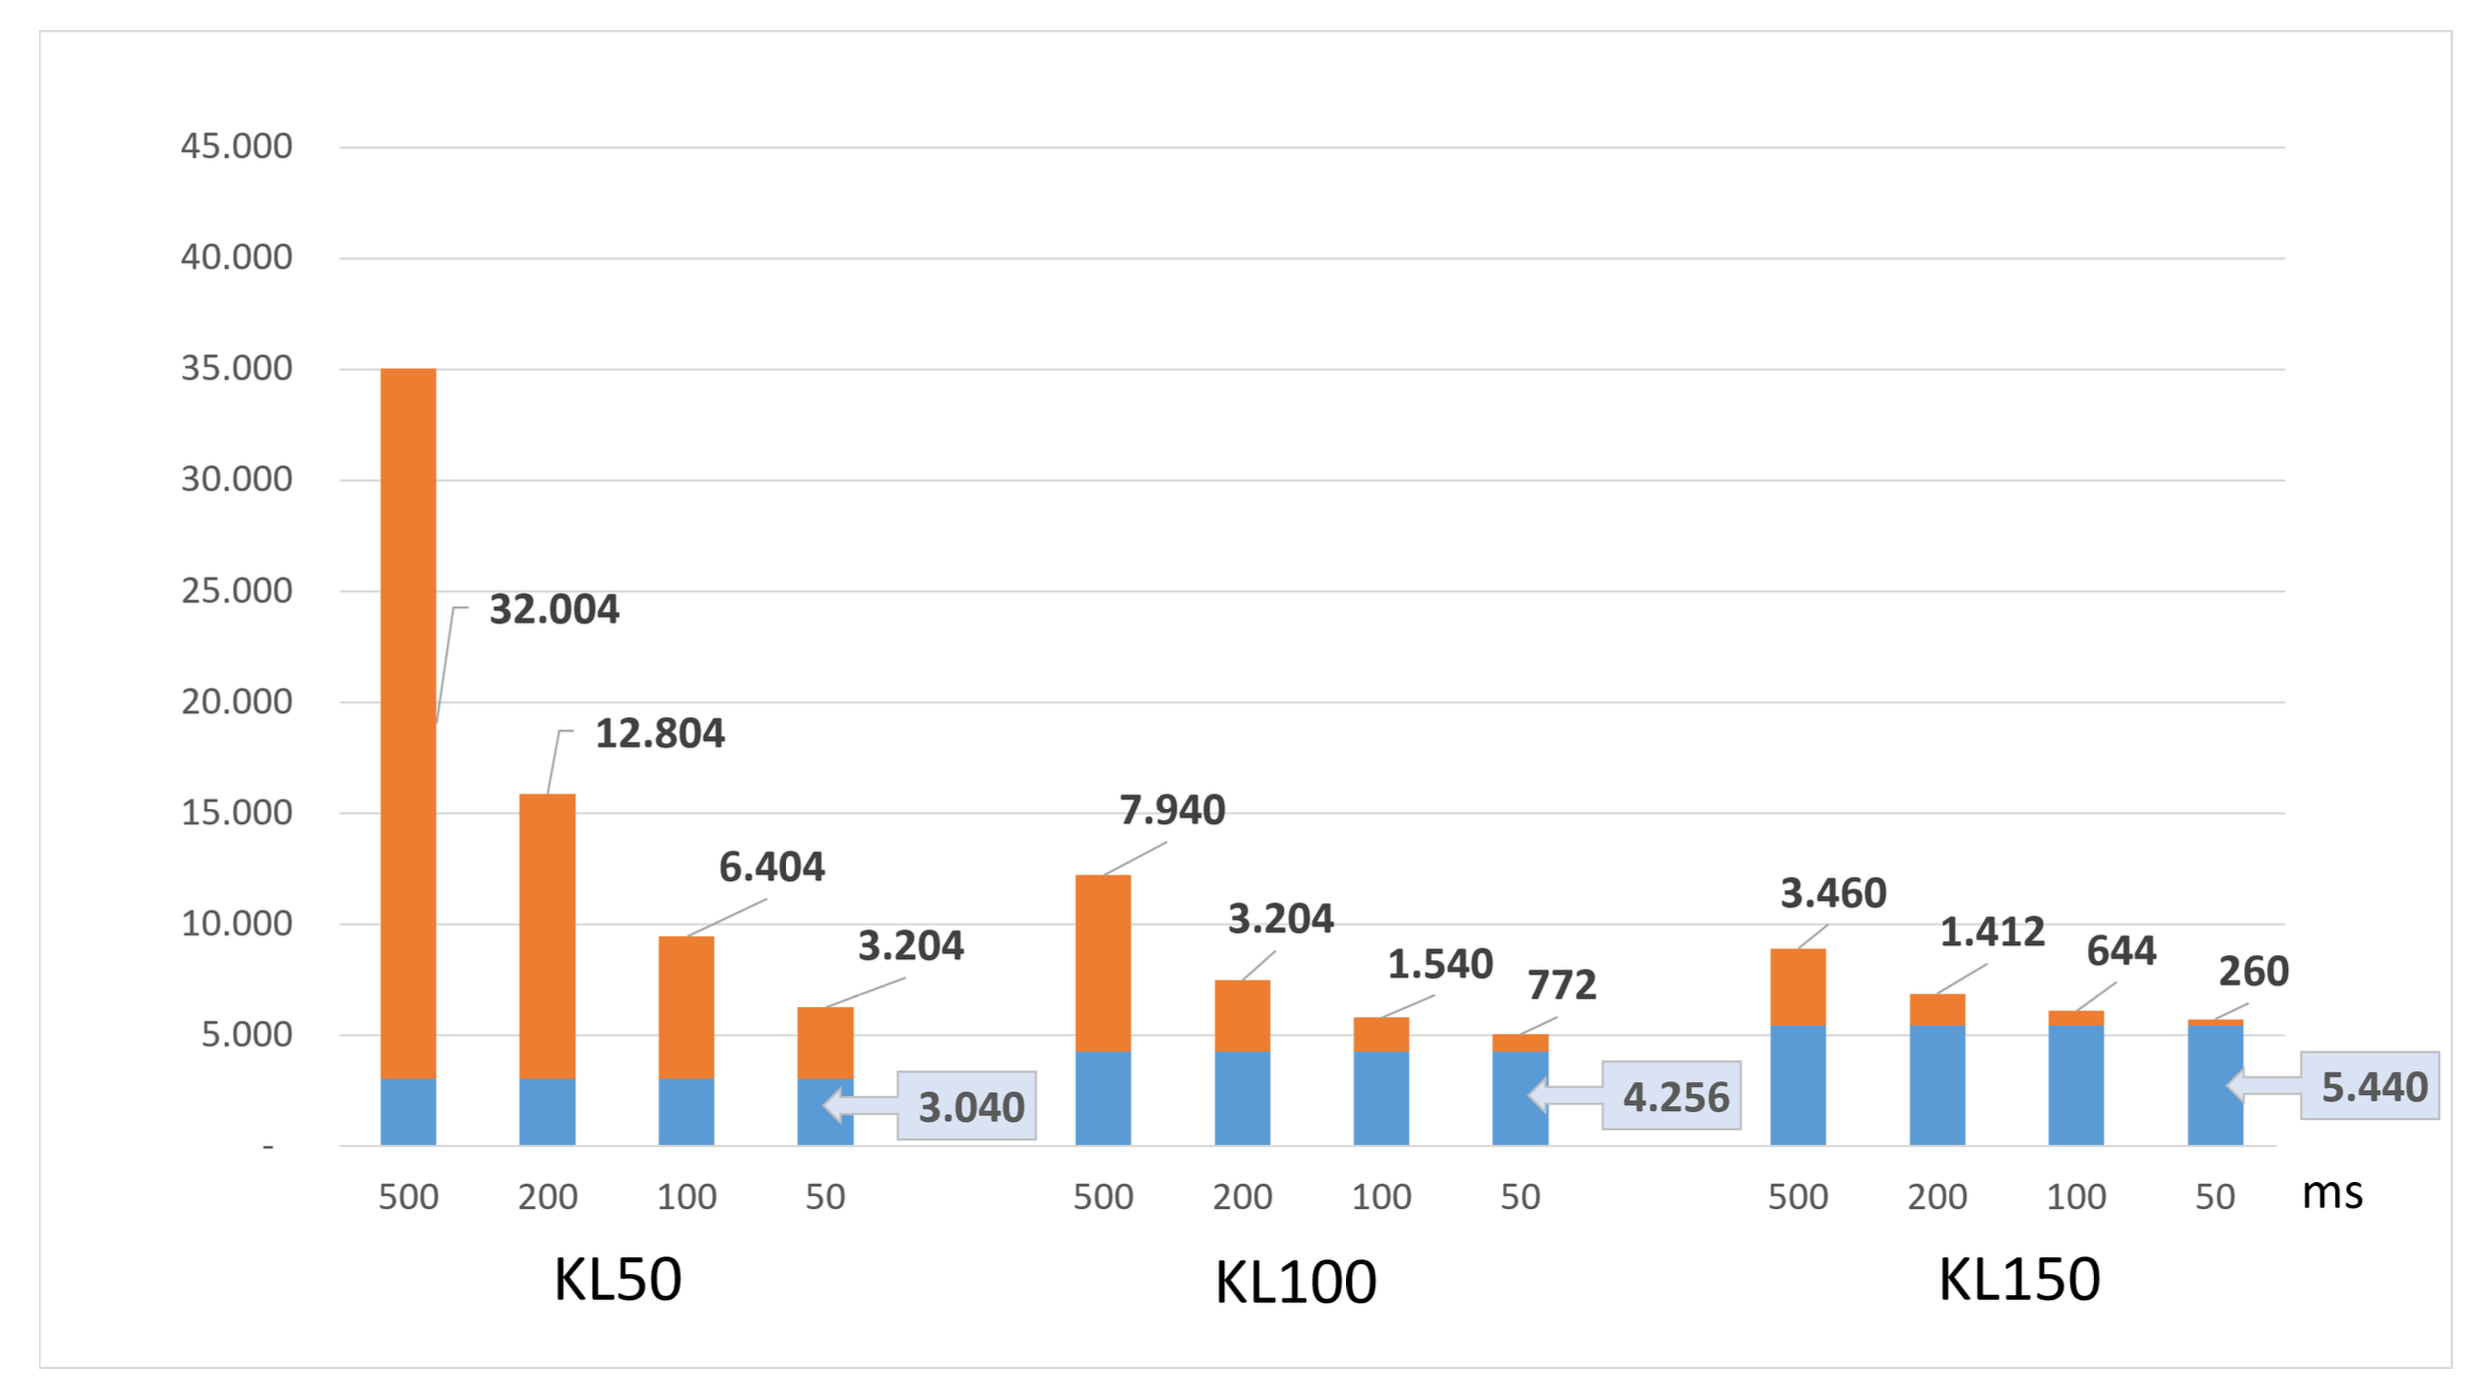
\includegraphics[scale=0.3]{engNet_params.png}
	\centering
\end{figure}

The number of parameters in a neural network is strictly related to the performance metrics of the network.
Given too many parameters a model will inevitably overfit to the training test and will therefore poorly generalize on the validation and test portion of the data. Conversely, too few parameters will make the model unable to learn effectively the classification required for the task at hand.
There is plenty of tools to overcome these kind of issues when training model, given that is one of the most prominent issues when dealing with neural networks performances such as tweaking the learning rate or adding dropouts layers in the architecture of the model in order to discard some of the parameters.
Clearly, reducing the number of parameters not only reduces the chances of overfitting but also decreases training and inference time.
Let us now delve deeper into the actual architecture.
The configuration for block 1 is as follows:
\begin{itemize}
\item Conv2D layer: Conv2D(, (1, kernLength), input shape=(Chans, Samples, 1))
\item AveragePooling2D layer: AveragePooling2D((1, kernLength//10))
\end{itemize}

Here, F1 represents the number of 2D convolutional filters (F1 = 16), Chans is the number of channels in the EEG signals (Chans = 16), and Samples is the length of the ENG samples. The Conv2D layer uses the kernel length to create a 2D convolutional filter with height 1 and width equal to kernLength. The AveragePooling2D layer reduces the spatial dimensions of the feature maps by performing average pooling with a pool size of (1, kernLength//10).

For block 2, the configuration is as follows:
\begin{itemize}
\item SeparableConv2D layer: SeparableConv2D(F2, (1, kernLength//4))
\item AveragePooling2D layer: AveragePooling2D((1, kernLength//25))
\end{itemize}

In block 2, the SeparableConv2D layer is used with a kernel size of (1, kernLength//4) and F2 = 32 to conduct depthwise separable convolution. This layer effectively reduces the number of parameters while preserving feature extraction capabilities. The parameters F1 and F2 are doubled compared to what was explained in chapter 3.5.1 and in [27] due to the larger frequency and consequently greater number of samples, while D remains equal to 2. This adjustment has been validated as a superior solution in preliminary tests.

\begin{figure}[H]
	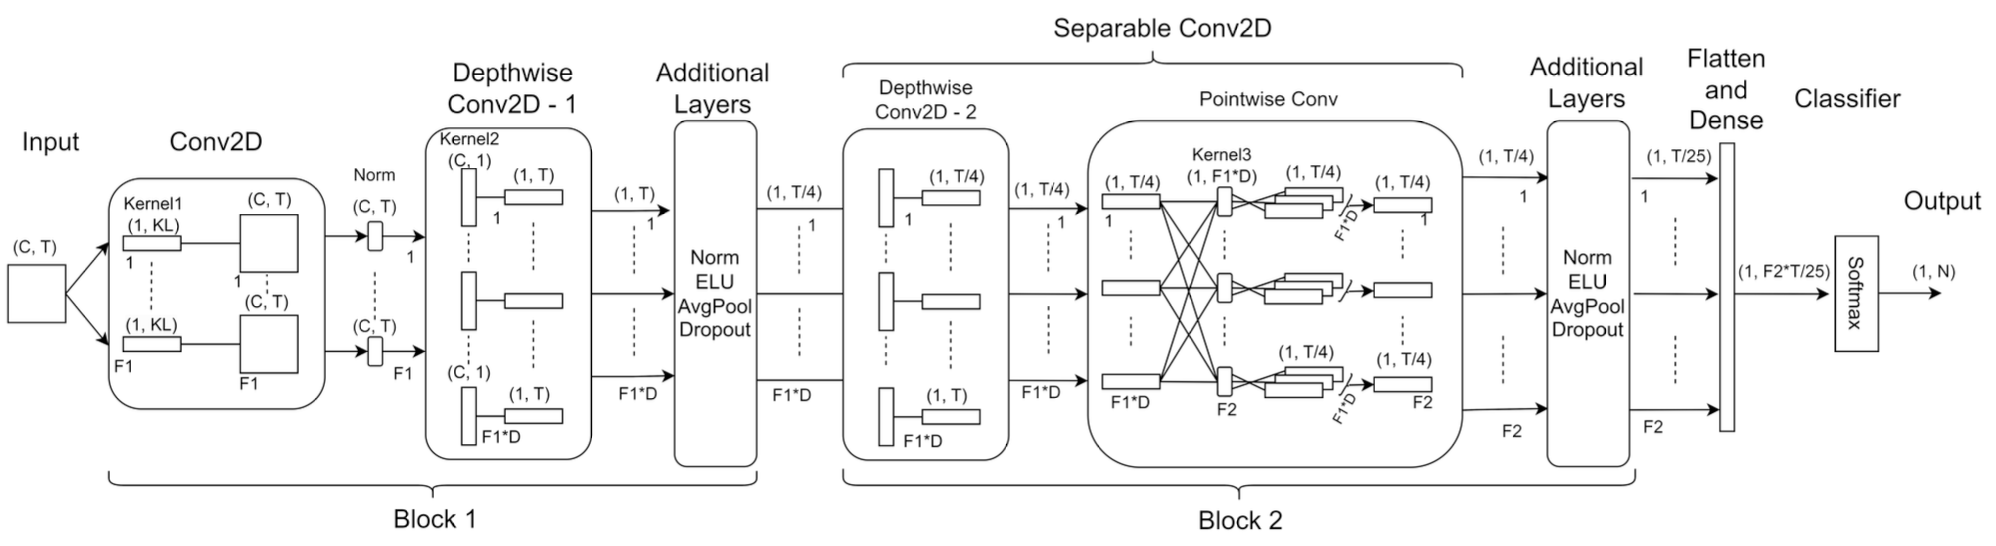
\includegraphics[scale=0.4]{engNet_arch.png}
	\centering
\end{figure}
	

\subsubsection{ENGNet layers}

We will now briefly explain the main layers present in the ENGNet model to outline what each layer does.



\begin{figure}[H]
	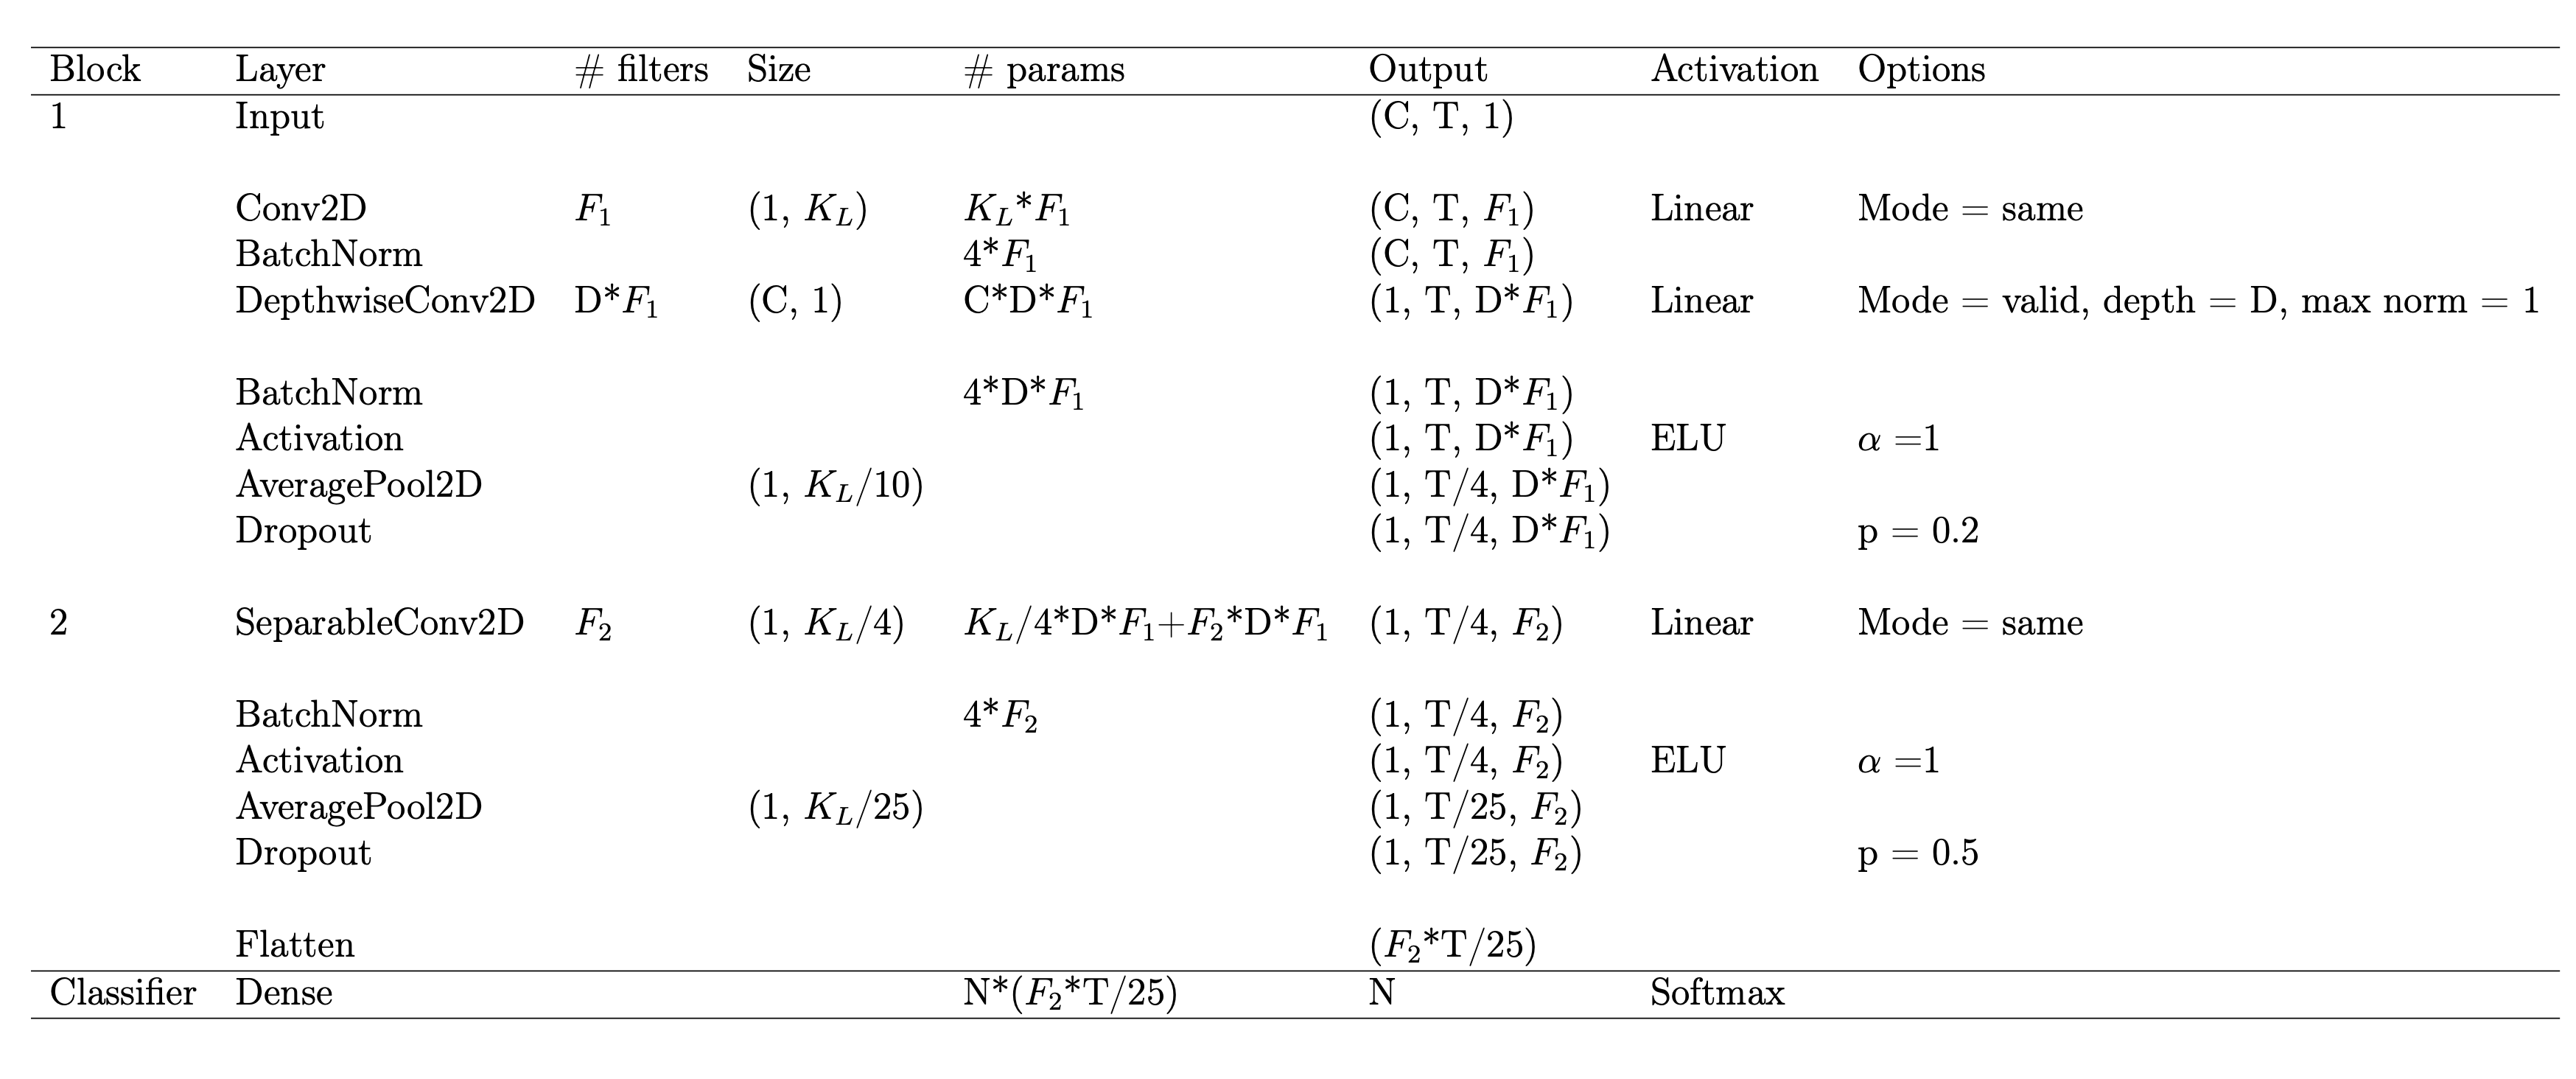
\includegraphics[scale=0.25]{engNet_layers.png}
	\centering
\end{figure}

\subsection{Classification performance metrics}

\textbf{Accuracy} \quad This measures the proportion of correctly classified examples in the dataset. It is calculated as:

\begin{equation}
\text{Accuracy} = \frac{\text{Number of Correct Predictions}}{\text{Total Number of Predictions}} \quad (3.21)
\end{equation}

\textbf{F1-Score} \quad It combines precision and recall to offer a balanced evaluation of a model’s performance. Precision (or Positive Predicted Value (PPV)) is the ratio of correctly predicted positive observations to the total predicted positive observations. Recall (or sensitivity, or True Positive Rate (TPR)), is the ratio of correctly predicted positive observations to the total actual positive observations. F1-Score is computed as:

\begin{equation}
F1 = 2 \cdot \frac{\text{Precision} \cdot \text{Recall}}{\text{Precision} + \text{Recall}} \quad (3.22)
\end{equation}

where:

\begin{equation}
\text{Precision (PPV)} = \frac{\text{True Positives}}{\text{True Positives} + \text{False Positives}} \quad (3.23)
\end{equation}

\begin{equation}
\text{Recall (TPR)} = \frac{\text{True Positives}}{\text{True Positives} + \text{False Negatives}} \quad (3.24)
\end{equation}

F1-Score combines precision and recall exploiting the harmonic mean to penalize the extreme values. Both Accuracy and the F1-score are important for a classification task:
\begin{itemize}
    \item Accuracy is preferred when correctly identifying True Positives and True Negatives is the primary concern.
    \item F1-score is favored when minimizing the impact of False Negatives and False Positives is crucial.
\end{itemize}

Moreover, when dealing with imbalanced class distributions, where some classes have significantly fewer instances than others, the F1-score tends to be a more suitable metric for model evaluation.


\textbf{Confusion Matrix} \quad This matrix visualizes a model’s performance by showing the number of true positives (TP), true negatives (TN), false positives (FP), and false negatives (FN). A general construction of confusion matrix is given in Table 3.1. It is particularly helpful for understanding the model’s ability to correctly classify each class and to investigate the errors in predict phase.

\begin{table}[h!]
\centering
\caption*{Table 3.1: Confusion Matrix for two classes (Positive and Negative) or outcomes to evaluate. The word "Predicted" refers to the output label from the classifier, while the "Actual" label is the one associated to the data.}
\begin{tabular}{|c|c|c|}
\hline
 & \textbf{Predicted Positive} & \textbf{Predicted Negative} \\
\hline
\textbf{Actual Positive} & TP & FN \\
\hline
\textbf{Actual Negative} & FP & TN \\
\hline
\end{tabular}
\end{table}

In a confusion matrix with multiple classes, it is possible to compute precision, recall, and the F1-score for each individual class. Precision for a class is calculated as the ratio of true positives for that class to the total instances predicted as that class (both true positive and false positives). It is calculated as the ratio of true positives to the sum of true positives and false positives for that class.

\begin{equation}
	\text{Precision (PPV)} = \frac{\text{True Positives}}{\text{True Positives} + \text{False Positives}} \quad (3.23)
	\end{equation}
	
	\begin{equation}
	\text{Recall (TPR)} = \frac{\text{True Positives}}{\text{True Positives} + \text{False Negatives}} \quad (3.24)
	\end{equation}

The F1-score is the harmonic of precision and recall. It provides a balanced measure that considers both false positives and false negatives. It is calculated using the following formula:

\begin{equation}
	F1 = 2 \cdot \frac{\text{Precision} \cdot \text{Recall}}{\text{Precision} + \text{Recall}} \quad (3.22)
	\end{equation}

By calculating these metrics for each class, one gains insights into the model’s performance for individual categories, allowing a more nuanced evaluation of classification effectiveness.



\subsection{ENGNet results}

\begin{figure}[H]
	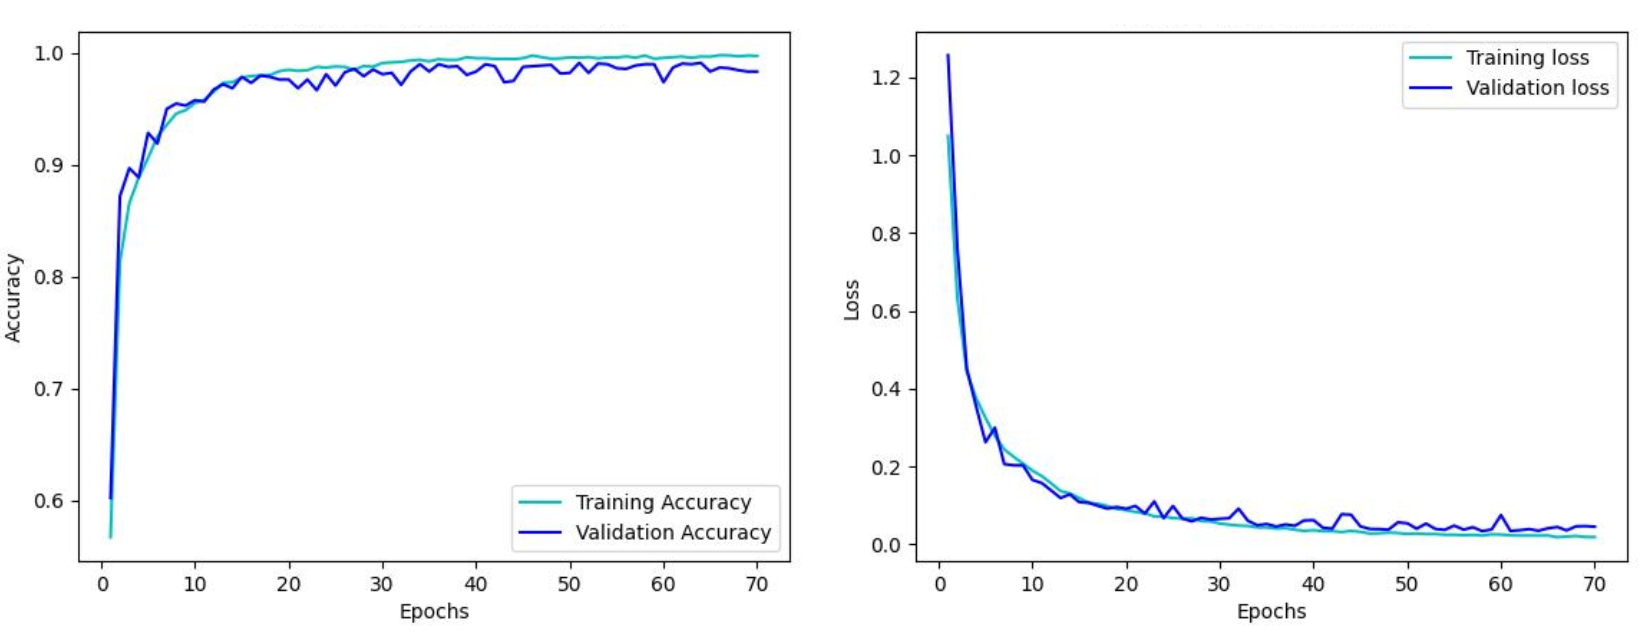
\includegraphics[scale=0.25]{trainingAccuracyDavide.png}
	\centering
	\end{figure}


Analysis of weights in the first convolutional layer indicate the network’s capability to recognize and accentuate characteristic ENG signal frequencies, and these are relevant to improves classification performance. However, the network’s ability to identify these frequencies depends on the quality of the signal used during training. The dependence of the power spectrum analysis on the data suggests the importance of carrying out specific training per subject, given that even within data taken from the same animal there is a variation in the frequencies emphasized by ENGNet,

\begin{figure}[H]
	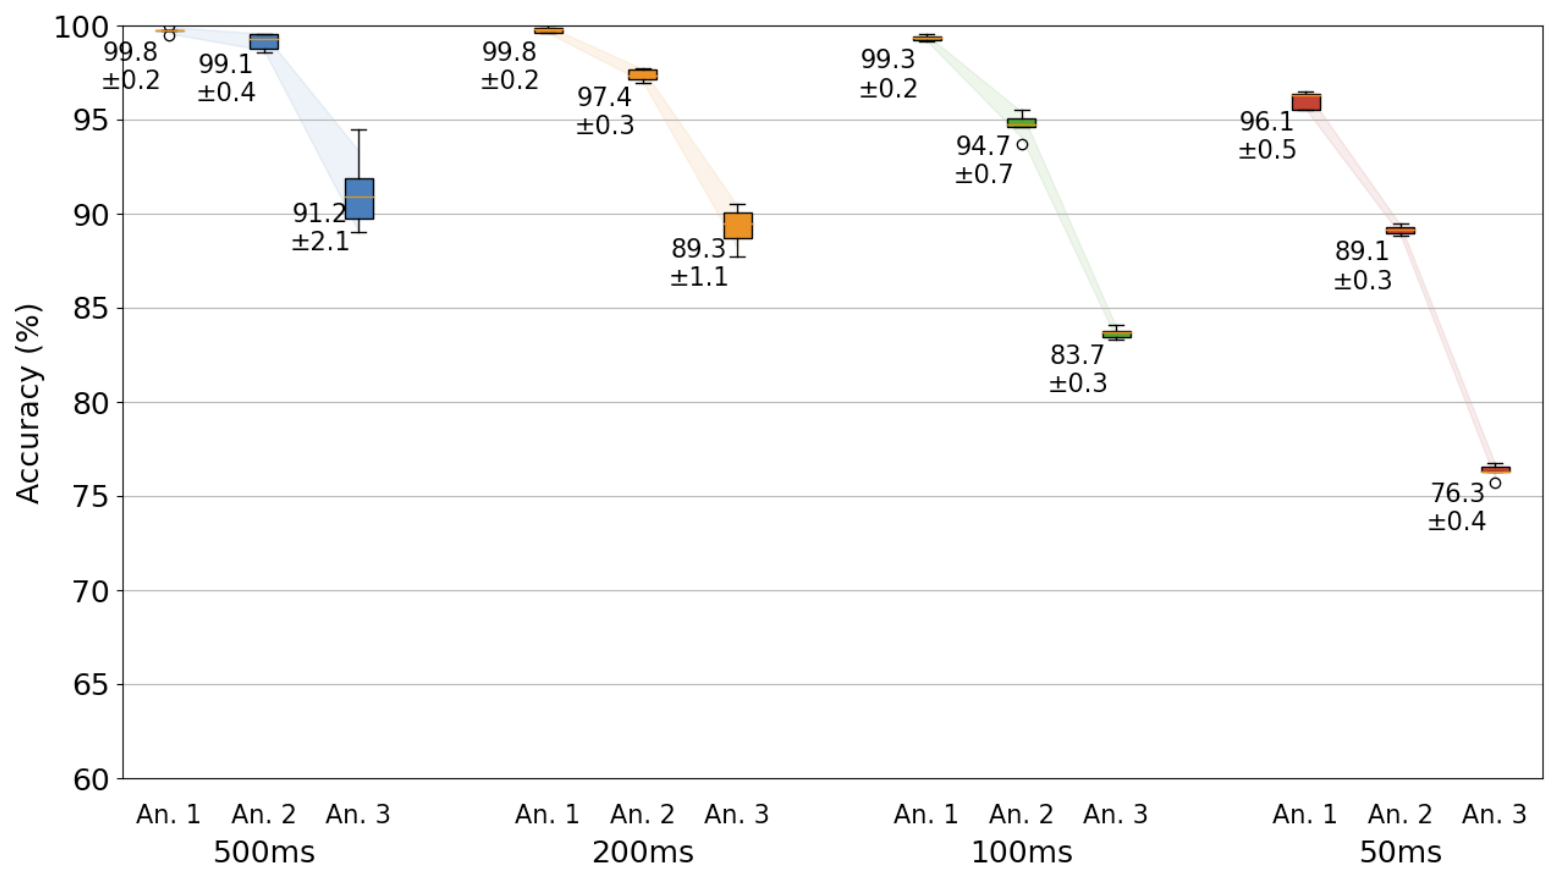
\includegraphics[scale=0.25]{engNet_accuracy.png}
	\centering
	\end{figure}
	
	\begin{figure}[H]
		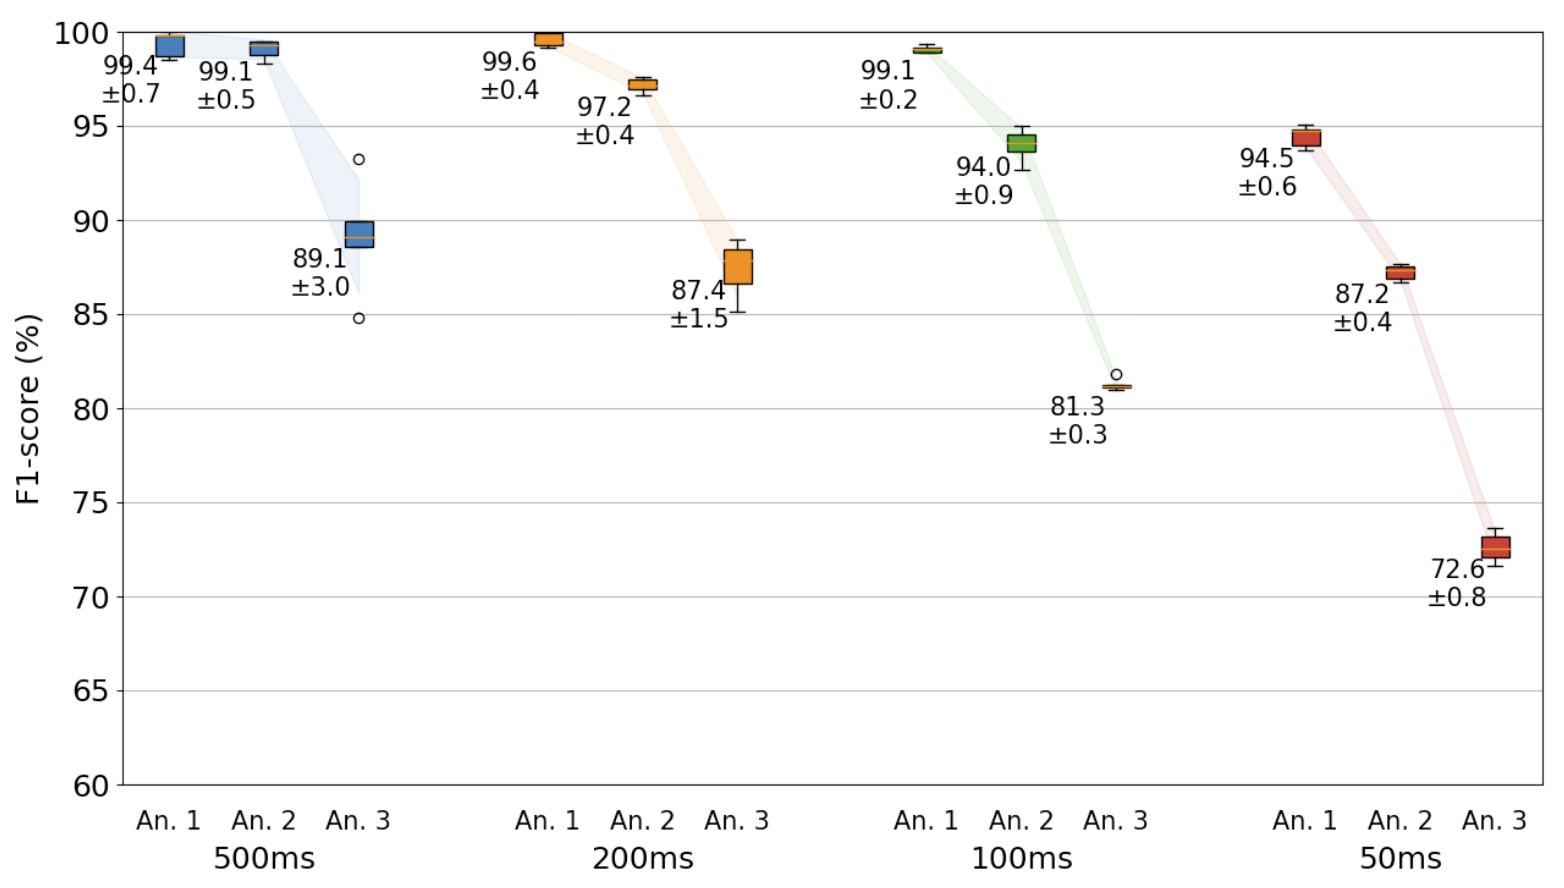
\includegraphics[scale=0.3]{engNet_f1score.png}
		\centering
		\end{figure}

Talk about limitation

Comparison between validation and test re- sults showed that ENGNet can generalize well to new data. This can be further improved by increasing the dropout probability


'foto dei results'



\section{nrf5280 Board pros and cons}
\section{Power Supplier}
\section{Memory management}

The memory architecture of the Nordic board is intricately designed to optimize performance and flexibility. The system comprises various memory regions and buses interconnected to facilitate efficient data transfer and processing. Below is a detailed explanation of each component illustrated in the provided diagram:

1. Central Processing Unit (CPU)
ARM Cortex-M4: The CPU is based on the ARM Cortex-M4 architecture, which is a highly efficient processor designed for high-performance, low-power applications. It includes a rich set of features such as floating-point unit (FPU), digital signal processing (DSP) extensions, and low-latency interrupt handling.
2. Memory Organization
The memory is divided into several sections, each serving a specific purpose and connected via different buses to optimize performance.

RAM Sections (AHB Slaves)
The system contains multiple RAM sections, each interfaced through the Advanced High-performance Bus (AHB). These sections are labeled from RAM0 to RAM8, with each section further divided into smaller subsections. The sections are organized as follows:

RAM0 to RAM8: These RAM sections are accessible via the System bus, DCODE, and ICODE buses, providing flexible access paths for different types of data operations. Each RAM section is split into two subsections (Section 0 and Section 1), and their memory addresses are specified for both data RAM (System) and code RAM (ICODE/DCODE).

Memory Addresses: The RAM sections have designated address ranges:

% Data RAM (System): Ranges from 0x2000_0000 to 0x2003_8000.
% Code RAM (ICODE/DCODE): Corresponding code addresses range from 0x0080_0000 to 0x0083_8000.
Flash Memory
Flash memory is used for non-volatile storage, providing persistent data retention even when the system is powered down. The flash memory is divided into pages and accessed via the ICODE and DCODE buses.

% Flash Pages: The flash memory is organized into pages, with the address range for flash starting at 0x0000_0000 and extending to 0x000F_F000.
Page Addresses: Specific addresses for pages include:
% Page 0: 0x0000_0000
% Page 1: 0x0000_1000
% Page 2: 0x0000_2000
Subsequent pages follow this addressing pattern up to Page 255.
3. Bus Architecture
The system utilizes a multilayer AHB interconnect to manage data flow between different components efficiently.

Advanced High-performance Bus (AHB)
The AHB multilayer interconnect ensures high-speed data transfer between the CPU, RAM sections, flash memory, and peripherals. It allows multiple masters (such as the CPU and DMA controllers) to access shared resources without significant performance bottlenecks.

System Bus, DCODE, and ICODE
These buses provide specific pathways for different types of data access:

System Bus: Used for general data transfers.
DCODE Bus: Dedicated to instruction fetches from flash memory.
ICODE Bus: Used for instruction fetches from both RAM and flash memory, enabling efficient code execution.
4. Peripherals and EasyDMA
Peripherals: The system includes various peripherals connected via the AHB2APB bridge, allowing integration with different peripheral devices.
EasyDMA: Direct Memory Access (DMA) controllers facilitate direct data transfers between peripherals and memory, bypassing the CPU to enhance efficiency. EasyDMA controllers are connected via DMA buses to the peripheral modules.
5. Address Mapping
The memory map clearly defines the address ranges for each memory section and peripheral, ensuring well-organized access to system resources.
RAM Sections: Each RAM section has a specific address range, both for system data and code execution, ensuring organized and conflict-free memory access.
6. Interconnect and Bus Matrix
The AHB multilayer interconnect/bus matrix allows concurrent access to different memory sections and peripherals, reducing latency and improving overall system throughput.

The Nordic board's memory architecture is a sophisticated system designed for efficient data handling and high performance. By leveraging multiple RAM sections, a well-organized flash memory layout, and an advanced bus interconnect system, the architecture supports the demanding requirements of modern embedded applications. The integration of DMA controllers further enhances data transfer efficiency, making the Nordic board suitable for a wide range of applications requiring reliable and high-speed memory access.

\section{Introduction}
The memory architecture of the Nordic board is intricately designed to optimize performance and flexibility. The system comprises various memory regions and buses interconnected to facilitate efficient data transfer and processing. This document provides a detailed analysis suitable for a thesis.

\section{Overview of the Address Map}
The address map is divided into two main sections: the System Address Map and the Address Map for peripherals. The System Address Map shows the hierarchical arrangement of different memory regions and device spaces, while the Address Map specifies the address ranges for peripherals and other key components.

\section{System Address Map}

\subsection{Device Space (0xE0000000 - 0xFFFFFFFF)}
This region is reserved for device-specific addresses, typically used for system control and private peripheral bus (PPB) mappings. The PPB includes critical control registers for system-level operations such as interrupts and debugging.

\subsection{RAM (0x80000000 - 0xBFFFFFFF)}
This region is designated for RAM, divided into two main blocks:
\begin{itemize}
    \item \textbf{0x80000000 - 0x9FFFFFFF}: General RAM space.
    \item \textbf{0xA0000000 - 0xBFFFFFFF}: Additional RAM or special-purpose RAM.
\end{itemize}

\subsection{Peripheral Space (0x60000000 - 0x7FFFFFFF)}
This area is allocated for peripheral devices, allowing the CPU to interact with various hardware modules via memory-mapped I/O.

\subsection{SRAM (0x40000000 - 0x5FFFFFFF)}
This region is dedicated to SRAM, providing fast, volatile memory storage for critical data that requires quick access times.

\subsection{Code Space (0x00000000 - 0x1FFFFFFF)}
This segment includes different types of memory used for storing executable code:
\begin{itemize}
    \item \textbf{0x00000000 - 0x007FFFFF}: Flash memory for non-volatile code storage.
    \item \textbf{0x00800000 - 0x00FFFFFF}: Code RAM for executing code from RAM.
    \item \textbf{0x10000000 - 0x10000FFF}: FICR (Factory Information Configuration Registers) containing device-specific configuration data.
    \item \textbf{0x12000000 - 0x12000FFF}: UICR (User Information Configuration Registers) for user-specific configuration.
    \item \textbf{0x19FFFFFF - 0x20000000}: XIP (Execute In Place) memory, allowing execution directly from external flash.
\end{itemize}

\section{Peripheral Address Map}

\subsection{Private Peripheral Bus (0xE0000000)}
The PPB includes system control space (SCS), NVIC (Nested Vectored Interrupt Controller), and other essential control registers.

\subsection{AHB Peripherals (0x50000000)}
This range is used for high-performance peripherals connected via the Advanced High-performance Bus (AHB), providing efficient data transfer capabilities.

\subsection{APB Peripherals (0x40000000)}
The Advanced Peripheral Bus (APB) space is designated for slower peripherals that do not require the high throughput provided by the AHB.

\section{Detailed Address Ranges and Usage}

\subsection{Flash Memory (0x00000000 - 0x007FFFFF)}
Used for storing the firmware and application code. Flash memory is non-volatile, retaining data even when power is off.

\subsection{Code RAM (0x00800000 - 0x00FFFFFF)}
Provides a space for loading and executing code from RAM, useful for applications requiring high-speed code execution.

\subsection{FICR (0x10000000 - 0x10000FFF)}
Contains factory-programmed data specific to the device, such as calibration values and unique identifiers.

\subsection{UICR (0x12000000 - 0x12000FFF)}
Stores user-programmable configuration data, which can include bootloader settings and memory protection configurations.

\subsection{XIP (0x19FFFFFF - 0x20000000)}
Allows the system to execute code directly from external flash memory, saving internal RAM for other uses.

\section{Summary}
The Nordic board's memory architecture is designed to efficiently manage various types of memory and peripheral access. The system address map and peripheral address map clearly define regions for devices, RAM, peripherals, and code execution. This structured organization allows for optimized performance, flexibility in code execution, and efficient interaction with peripherals.

By understanding this memory layout, developers can make informed decisions about memory usage, peripheral integration, and system optimization, ultimately enhancing the performance and functionality of applications running on the Nordic board.

Based on the detailed analysis of the Nordic board's memory architecture, several key observations can be made to optimize code and effectively manage memory. These recommendations will help developers enhance the performance and efficiency of their applications.

\section{Observations and Recommendations}

\subsection{Utilizing Flash Memory for Code Storage}
\textbf{Observation:}
\begin{itemize}
    \item Flash memory (0x00000000 - 0x007FFFFF) is non-volatile and ideal for storing the firmware and application code.
\end{itemize}

\textbf{Recommendation:}
\begin{itemize}
    \item Store all static code and infrequently updated data in flash memory to ensure data persistence across reboots and power cycles.
    \item Optimize the code to minimize the frequency of flash writes, as flash memory has a limited number of write cycles.
\end{itemize}

\subsection{Efficient Use of Code RAM}
\textbf{Observation:}
\begin{itemize}
    \item Code RAM (0x00800000 - 0x00FFFFFF) allows for high-speed code execution.
\end{itemize}

\textbf{Recommendation:}
\begin{itemize}
    \item Load performance-critical code segments and frequently accessed functions into Code RAM to benefit from faster execution times.
    \item Use this space judiciously due to its limited size, prioritizing code that requires low-latency access.
\end{itemize}

\subsection{Managing Volatile Data with SRAM}
\textbf{Observation:}
\begin{itemize}
    \item SRAM (0x40000000 - 0x5FFFFFFF) provides fast, volatile memory for temporary data storage.
\end{itemize}

\textbf{Recommendation:}
\begin{itemize}
    \item Use SRAM for variables, stack, and heap allocation that require quick read/write access.
    \item Regularly monitor SRAM usage to prevent stack overflows and ensure efficient memory allocation.
\end{itemize}

\subsection{Leveraging XIP for External Code Execution}
\textbf{Observation:}
\begin{itemize}
    \item XIP (0x19FFFFFF - 0x20000000) enables execution directly from external flash memory.
\end{itemize}

\textbf{Recommendation:}
\begin{itemize}
    \item Utilize XIP for large codebases or rarely executed code to free up internal RAM and Flash memory.
    \item Ensure that the execution speed from external memory meets the application's performance requirements.
\end{itemize}

\subsection{Using FICR and UICR for Configuration Data}
\textbf{Observation:}
\begin{itemize}
    \item FICR (0x10000000 - 0x10000FFF) and UICR (0x12000000 - 0x12000FFF) store factory and user-specific configuration data, respectively.
\end{itemize}

\textbf{Recommendation:}
\begin{itemize}
    \item Store device-specific and user-defined configuration settings in FICR and UICR.
    \item Use these regions to keep calibration data, unique identifiers, and bootloader settings.
    \item These registers should be written infrequently to avoid wear.
\end{itemize}

\subsection{Optimizing Peripheral Access}
\textbf{Observation:}
\begin{itemize}
    \item AHB (0x50000000) and APB (0x40000000) peripheral spaces are designated for high and low throughput peripherals.
\end{itemize}

\textbf{Recommendation:}
\begin{itemize}
    \item Map high-speed peripherals that require frequent access to the AHB space for efficient data transfers.
    \item Use the APB space for peripherals with lower bandwidth requirements.
    \item Ensure that peripheral access patterns do not create bottlenecks, particularly in real-time applications.
\end{itemize}

\subsection{Balancing RAM and Peripheral Usage}
\textbf{Observation:}
\begin{itemize}
    \item The board has multiple RAM sections and peripheral regions connected via AHB and APB buses.
\end{itemize}

\textbf{Recommendation:}
\begin{itemize}
    \item Distribute memory usage across different RAM sections to avoid contention and ensure balanced load.
    \item Efficiently manage DMA transfers to minimize CPU involvement in data movement between peripherals and memory, thus improving overall system performance.
\end{itemize}






Our boards, the nRF52840 contain 1024 kB of flash memory and 256 kB of RAM, they can be used for both code and data storage. [https://infocenter.nordicsemi.com/index.jsp?topic=%2Fps_nrf52840%2Fmemory.html]

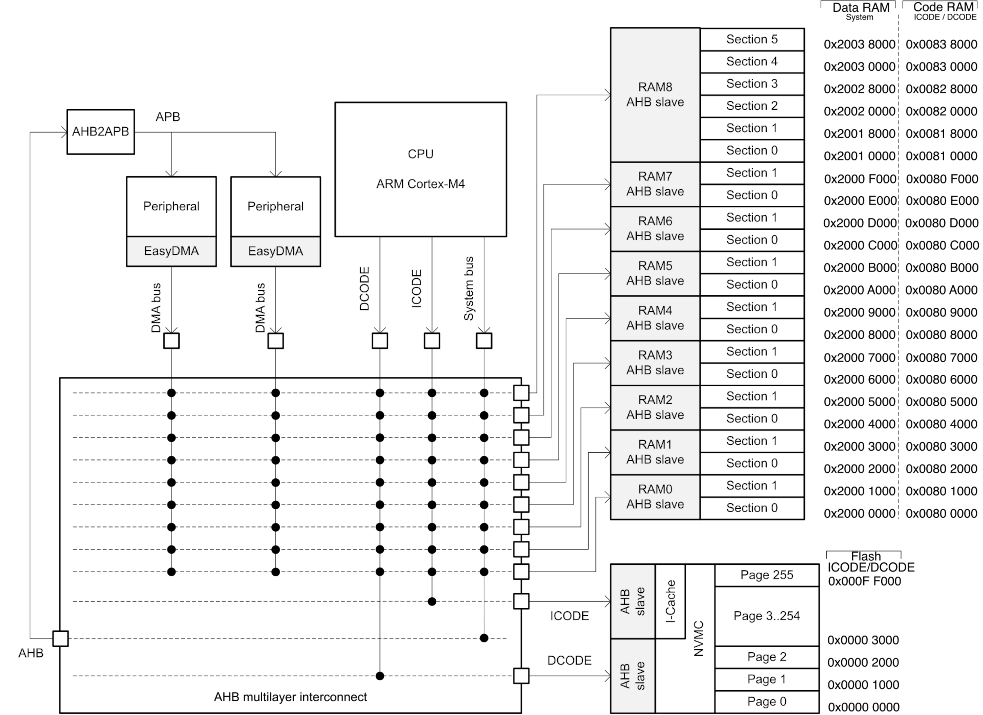
\includegraphics[scale=0.3]{memNRF.png}
\begin{figure}[H]
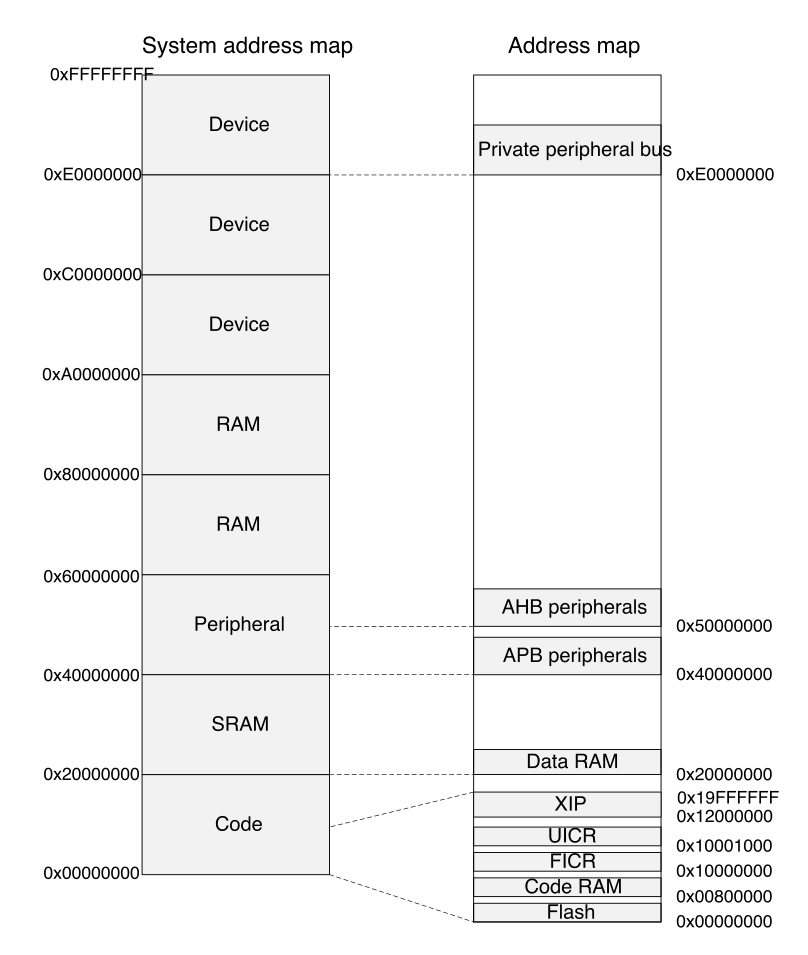
\includegraphics[scale=0.4]{memory2.png}
\centering
\end{figure}


Structure of the board memory, many images to describe ram.
No cache
Why no cache is a problem and why it is ok.
What devices have caches maybe.
Show a couple methods to avoid programmer control over memory managment from paper.
We could include metrics later if we have time, like space occupied and shit and if we can reduce that.







\section{Radiation absorbtion}
\section{Channel selection}

We have already described in previous sections the project at hand and why every possible improvement can ease the development of a functional implementation.
One of those crucial aspects is the amount of information sent between the devices, in the particular the channels that get transmitted.
As previously shown, the dataset at hand was registered using cuff electrodes chirurgically implanted on the animals' peripheral nerves; each of these cuff electrodes has 16 sensors that are able to measure the voltage of the nerve they cover.
Each of these sensors, being in a different position, will register different data, furthermore one or more of these sensors may be damaged during the surgery or may record data with high noise.
Because of this, not only it would be useful to limit the channel we share between devices to help with the communication, but we could also help the classifier by removing channels with faulty or noisy sensors.
In short, the three benefits of channel selection are : reducing the computational complexity of any process on the dataset, reduce the amount of overfitting of the models and reudce the times to setup the application. \cite{alotaibyReviewChannelSelection2015}
There is a great amount of literature that deals with the issues of channel selection of EEG channels, since it is a well known area of research and proves to be very helpful in reaching better results.
In particular our area of interest focused on channel selection applied to motion-imagery EEG Signals (MI-EEG).
We will now present an overview of the most relevant methods for channel selection.

\subsection{Common spatial patterns methods}

Common spatial patterns (CSP) method was firstly suggested for classification of multi-channel EEG during imagined hand movements by H. Ramoser \cite{ramoserOptimalSpatialFiltering2000}. The core concept involves employing a linear transformation to map multi-channel EEG data into a reduced-dimensional spatial realm using a projection matrix. Each row of this matrix represents channel weights. This process aims to optimize the variance of signal matrices for two classes. The CSP method relies on concurrently diagonalizing the covariance matrices of both classes. \cite{abdullahEEGChannelSelection2022}

Let X $\epsilon$ $R^{M x N}$ denote a matrix of EEG, where the channel number is M and the samples are denoted by N. The classic CSP problem is stated as follows:

\begin{align}
	\max_{W \epsilon R^{M}} = \frac{W^{T} C_1 W}{W^{T} C_2 W}
	\label{eq:CSP1}
\end{align}

where W is a spatial filter coefficient, $C_{i}$(i=1,2) indicates a single-class covariance matrix. The generalised eigenvalue decomposition (EVD) generally can handle this problem. \cite{abdullahEEGChannelSelection2022}

\subsubsection{Sparse CSP}

Due to classic CSP inadequacies, several researchers aim to integrate sparsing behavior with conventional CSP to discover and eliminate highly noisy or interfering channels. Given w’s sparsity k, i.e., the number of nonzero items in w. The sparse CSP problem is stated as follows:

\subsubsection{Regularized CSP}

% Despite its well-established efficacy and widespread adoption, CSP is acknowledged for its susceptibility to noise and tendency for overfitting. To tackle this concern, researchers have proposed the regularization of CSP \cite{lotteRegularizingCommonSpatial2011}. A recommended strategy is the adoption of a regularized CSP (RCSP) approach, which focuses on regulating the covariance matrix estimate within CSP extraction. This involves employing regularization techniques derived from general learning principles \cite{friedmanRegularizedDiscriminantAnalysis1989,wangSolvingFaceRecognition2006}. The regularization of CSP can occur at two levels, the first being at the estimation of the covariance matrix. Since CSP relies on these estimates, which can be adversely affected by noise or limited training data, regularization can significantly improve performance. Alternatively, regularization can be implemented at the objective function level (Eq. 1), where spatial filters are subjected to prior constraints to enhance stability \cit{lotteRegularizingCommonSpatial2011}.

% The first, based on \cite{luRegularizedCommonSpatial2009} can be implemented in the following way:

\begin{align}
	\tilde{C}_{C} = (1 - \gamma) \hat{C}_{C} + \gamma I
	\label{eq:RCSP1}
\end{align}

\begin{align}
	\hat{C}_{C} = (1 - \beta) {s}_{C} {C}_{C} + \beta {G}_{C}
	\label{eq:RCSP2}
\end{align}


% where $C_{c}$ is the initial spatial covariance matrix for class $c$, $\tilde{C}_{c}$ is the regularized estimate, $I$ is the identity matrix, $S_{c}$ is a constant scaling parameter (a scalar), $\gamma$ and $\beta$ are the two user-defined regularization parameters ($\gamma$, $\beta \in [0,1]$), and $G_{c}$ is a “generic” covariance matrix. \cite{lotteRegularizingCommonSpatial2011}

Another approach to obtain RCSP algorithms consists in regularizing the CSP objective function itself (1). More precisely, such a method consists in adding a regularization term to the CSP objective function in order to penalize solutions (i.e., resulting spatial filters) that do not satisfy a given prior. Formally, the objective function becomes:

\begin{align}
	{J}_{P_{1}}(w) = \frac{w^{T}C_{1}w}{w^{T}C_{2}w + \alpha P(w)}
	\label{eq:RCSP3}
\end{align}

% where P(w) is a penalty function, measuring how much the spatial filter w satisfies a given prior. The more w satisfies it, the lower P(w). Hence, to maximize JP1(w), we must minimize P(w), thus ensuring spatial filters satisfying the prior. $\alpha$ is a user-defined regularization parameter ( $\alpha$ $\geq$  0, the higher $\alpha$, the more satisfied the prior). With this regularization, we expect that enforcing specific solutions, due to priors, will guide the optimization process toward good spatial filters, especially with limited or noisy training data. \cite{lotteRegularizingCommonSpatial2011}


% ciao \ref*{cap}

\subsection{Correlation-based methods}

These methods help identifying which subsets of channels is the most relevant by defining a correlation metric and ranking higher those channels that show stronger similarities between them according to the metric.
There are various ways in which we can score the correlation between signals of different channels and here we will briefly present three.

\subsubsection{Spectral entropy dunno first citation}

Spectral entropy is a generic measure of disorganization of signal, as expressed in \cite{yangEEGChannelSelection2018b} with the following formulas:

\begin{align}
H(E)=-\sum_{i=1}^N p\left(E_i\right) \log _{10} p\left(E_i\right),
\end{align}

where \( \mathcal{E} = \{ \mathcal{E}_1, \mathcal{E}_2, \ldots, \mathcal{E}_n \} \) is the signal in the time domain. \( p(\mathcal{E}_i) \) is the probability of \( \mathcal{E}_i \). It is usually estimated by Burg's algorithm. \cite{schalkBCI2000GeneralpurposeBraincomputer2004} \\
Spectral entropy separates the background noise from the organized signal, the motor imagery in this study.

The 'interested class versus the rest' strategy is adopted for the channel selection using the correlation coefficient method. EEG data are split into two groups, \( s_1 \) and \( s_2 \), where \( s_1 \) is the group containing the class of interest. \\
Spectral entropy \( H_1 \) and \( H_2 \) are identified corresponding to \( s_1 \) and \( s_2 \). Correlation of the spectral entropy from the two groups, \( s_1 \) and \( s_2 \), is an indicator of how closely these two groups have a linear relationship, written as:

\begin{align}
\rho\left(H_{1, j}, H_{2, j}\right)=\frac{\operatorname{cov}\left(H_{1, j}, H_{2, j}\right)}{\sigma_{H_1, j} \sigma_{H_2, j}},
\end{align}

where \( \sigma_{H_j} \) is the standard deviation of the respective spectral entropy. \( j \) is the index of the channel. \\
 For the purpose of channel selection, we consider the spectral entropy of each channel across all frequency ranges by taking the sum of the squared correlation coefficient,

\begin{align}
P\left(H_{1, j}, H_{2, j}\right)=\sum_{i=1}^N \rho^2\left(H_{1, j}, H_{2, j}\right),
\end{align}

where $i$ = 1 - $N$ is the number of frequency bins during estimation of the spectral entropy.

\subsubsection{Pearson’s Correlation Coefficient }

Pearson correlation coefficient is a statistical association or linear dependence between two or more random variables and, in our case, it can measure the linear correlation between two channels. \cite{thibeaultUsingHybridNeuron2013}


\begin{align}
	\rho (X,Y) = \frac{1}{n-1} \sum_{i}^{N}(\frac{X_i - \bar{X}}{\sigma_{X}})( \frac{Y_i - \bar{Y}}{\sigma_{Y}})
	\label{eq:correlationCoefficient}
\end{align}

Considering the two variables, denoted as \( X \) and \( Y \), with \( n \) representing the number of observations, \( \bar{X} \) and \( \bar{Y} \) as their respective means, and \( \sigma_X \) and \( \sigma_Y \) as the default deviations between them, the correlation coefficient \( \rho(X,Y) \) ranges from 0 to 1. This range indicates the strength of the relationship, varying from low to high. In this context, the correlation coefficient is computed for each pair of EEG channels.

\subsubsection{Cross-Correlation Based Discriminant Criterion (XCDC)}

XCDC is another correlation method whose fundamental idea is that if a channel is informative and useful for the classification task at hand, then it should be highly correlated 


Given two finite discrete time series $x(i)$ and $y(j)$
(i $\epsilon$ $[0, 1, . . . , n - 1]$, j $\epsilon$ $[0, 1, . . . , m - 1]$, $m \geq n$),
their cross-correlation series is given as follows:

\begin{align}
	 r_{xy}(k) = \sum_{i=0}^{n-1}x(i)y(i + k), k = 0,1,...,m-n+1
	\label{eq:XCDC1}
\end{align}

where x and y are EEG signals of length T (m=n=T). \\ 
Zero-padding is performed at both sides of y so that the length of the cross-correlation series is the same of the original signals. \\
We apply the cross-correlation formula to the signals x and y, but we must firstly apply z-score normalization to account for the effect of signal amplitudes on cross-correlation.

\begin{align}
	\tilde{x_i} = \frac{x_i - \bar x_i}{\sigma_{x_i}}
   \label{eq:XCDC3}
\end{align}


Then, the similarity between x and y is measured with the following formula:

\begin{align}
	S(x,y) = \max(r_{x\hat{y}(k)}), k=0,1,..., T - 1 
   \label{eq:XCDC2}
\end{align}

with $\hat{y}$ being y with zero-padding.
where $x_i$ is the signal of the i-th trial collected from our channel of interest. $\bar{x_i}$ and $\sigma{x_i}$ are
the mean and standard deviation of $x_i$ respectively.
Having defined the function $S$ we now define the within-class similarity $R_w$ and betweenclass dissimilarity $R_b$ which are obtained as follows:

\begin{align}
	R_w = \mathbf{mean}(S(\tilde{x_i}\tilde{x_j}| c_i = c_j))
   \label{eq:XCDC4}
\end{align}

\begin{align}
	R_b = -\mathbf{mean}(S(\tilde{x_i}\tilde{x_j}| c_i \neq  c_j))
   \label{eq:XCDC5}
\end{align}

where $c_i$ is the class label of the i-th trial. The discriminant score D is then defined as follows:

\begin{align}
	D = \lambda R_w + (1-\lambda)R_b
   \label{eq:XCDC6}
\end{align}

in which $\lambda$ is a weighting hyperparameter to be tuned empirically.
Channels are ranked in a descending order according to their discriminant score D after obtaining D for every channel using.

\begin{table}[H]
	\caption{Accuracy for correlation based methods}
	\begin{tabular}{|p{2cm}|p{2cm}|p{2cm}|p{2cm}|p{2cm}|p{2cm}|}
	\hline
	Methods & Methods' stategy & Classifier &Accuracy&No. of Selected Channels/Total No. of Channels&Dataset\\
	\hline
	Afghanistan   & AF    &AFG&   004&   004&   004\\
	Afghanistan   & AF    &AFG&   004&   004&   004\\
	\hline
	\end{tabular}
	\end{table}
\subsection{Sequential Based methods}

These methods implement a sequential approach where top features are identified iteratively.
The most common example of Sequential method is the Sequential Forward Selection that was first used for variable selection by Whitney (1971). \\
It begins the research with an empty set of features, all the features are evaluated according to their impact on the evaluation metric and then, the variable with the best effect gets added to the subset of features. \\
This step gets re-iterated untill all the variables are progressively included in the set for comparisons purposes.
SFS has what is defined as the "nesting property" which means that once a feature gets included in the subset, that feature stays in the subset even if removing it would improve the results.  \cite{reunanenOverfittingMakingComparisons}
A different version is the Sequential Backward Search which functions identically but starts from a full set of variables and removes one them one by one according to the worst impact on the evaluation metrics. \cite{pudilFloatingSearchMethods1994} \\
Both of these methods' complexity is O($n^2$). \cite{kudoComparisonAlgorithmsThat2000}

\subsubsection{Sequential Floating Forward Selection (SFFS)}

The sequential forward floating selection has in many instances demonstrated to be a superior algorithm.\cite{reunanenOverfittingMakingComparisons} \cite{zongkerAlgorithmsFeatureSelection1996}
In our case in particular by addressing the nesting issue we better account for two features that highly impact the evaluation metrics but being highly correlated effectively carry the same information and may be not be both relevant to the final subset of features.
It returns a better subset of feature at the cost of a higher complexity of O($2^n$). \cite{kudoComparisonAlgorithmsThat2000} \\
The core approach utilized in Sequential Floating Forward Selection (SFFS) to address nesting issues involves initiating a backtracking phase after the addition of each variable. During this phase, variables are systematically excluded until superior subsets of corresponding sizes are identified. This process continues until no better subset is discovered, prompting a return to the initial step to include the best previously excluded variable. Subsequently, another backtracking phase ensues. \cite{reunanenOverfittingMakingComparisons} \cite{ pudilFloatingSearchMethods1994} \\ 
In the original work of Pudil (1994) it is also proposed a floating version of the SBS called SBFS that implements the same idea but once again starting with a full set of features and removing them iteratively. Its complexity is O($2^n$).

\subsubsection{Generalized Sequential Forward Selection (GSFS) }

Generalized Sequential Forward Selection (GSFS) is an extension of the Sequential Forward Selection (SFS) algorithm. \\
In GSFS, similar to SFS, the algorithm starts with an empty set of features and iteratively adds features to the model based on some evaluation criterion, such as minimizing error or maximizing predictive performance. However, GSFS introduces additional flexibility by allowing the inclusion of multiple features at each step instead of just one. This can potentially speed up the feature selection process and lead to better performance by considering feature combinations more efficiently.

The key idea behind GSFS is to explore feature subsets in a more generalized manner, considering not only individual features but also combinations of features at each step of the selection process. This can be particularly useful in situations where interactions between features are important for modeling complex relationships in the data.

Overall, GSFS offers a more flexible and comprehensive approach to feature selection compared to traditional forward selection methods like SFS, making it suitable for a wide range of applications in machine learning and data analysis. \cite{radmanGeneralizedSequentialForward2019}
GSFS and the backward implementation GSBS, both have a complexity that depend of the number of features they can add per iteration, if we define g as the number of features added per iteration, then their complexity is O($n^{g+1}$). \\
 With g = 1 GSFS is equal to SFS.

\subsection{Binary Particle Swarm Optimization Based methods}

In 1995, the PSO algorithm was presented by Kennedy and Eberhart. \cite{okwuMetaheuristicOptimizationNatureInspired2020} \\
The idea behind it is inspired by the social behavior of birds flocking or fish schooling. \cite{vanneschiParticleSwarmOptimization2023}
In standard PSO, particles move around in a continuous solution space, adjusting their positions and velocities based on their own best-known position and the global best-known position found by any particle in the swarm.
\\
This collective learning process guides the particles toward better regions of the search space, converging to the optimal solution. \\
The balance between exploration (searching for new solutions) and exploitation (refining known solutions) is controlled by various parameters such as inertia weight, cognitive factor, and social factor. \\
Example update functions for position ($x_{i}(t+1)$) and speed ($v^{i}_{k+1}$) are as follows from Abdullah\cite{abdullahEEGChannelSelection2022}:

\begin{align}
	v_{k+1}^i=w v_k^i+c_1 r_1\left(p_k^i+x_k^i\right)+c_2 r_2\left(g b e s t-x_k^i\right)
	\label{eq:bpso1}
\end{align}
\begin{align}
	x_i(t+1)=x_i t+v_i(t+1)
	\label{eq:bpso2}
\end{align}

where i represents the i-th particle. $c_1$ is the cognitive coefficient and $c_2$ is the social one. They regulate how fast the particle is going and are both constant. $w$ is the inertial weight which limits the speed. $r_1$,$r_2$ are random values between 0 and 1. $k$ represents the iteration of the update function. $t$ represents the time. $p^{i}_{k}$ represents the best solution found so far by the i-th particle at k-th iteration. gbest is the best position found by the swarm so far.
Just below we present a visualization of particle movement in a 3D space. 

\begin{figure}[H]
	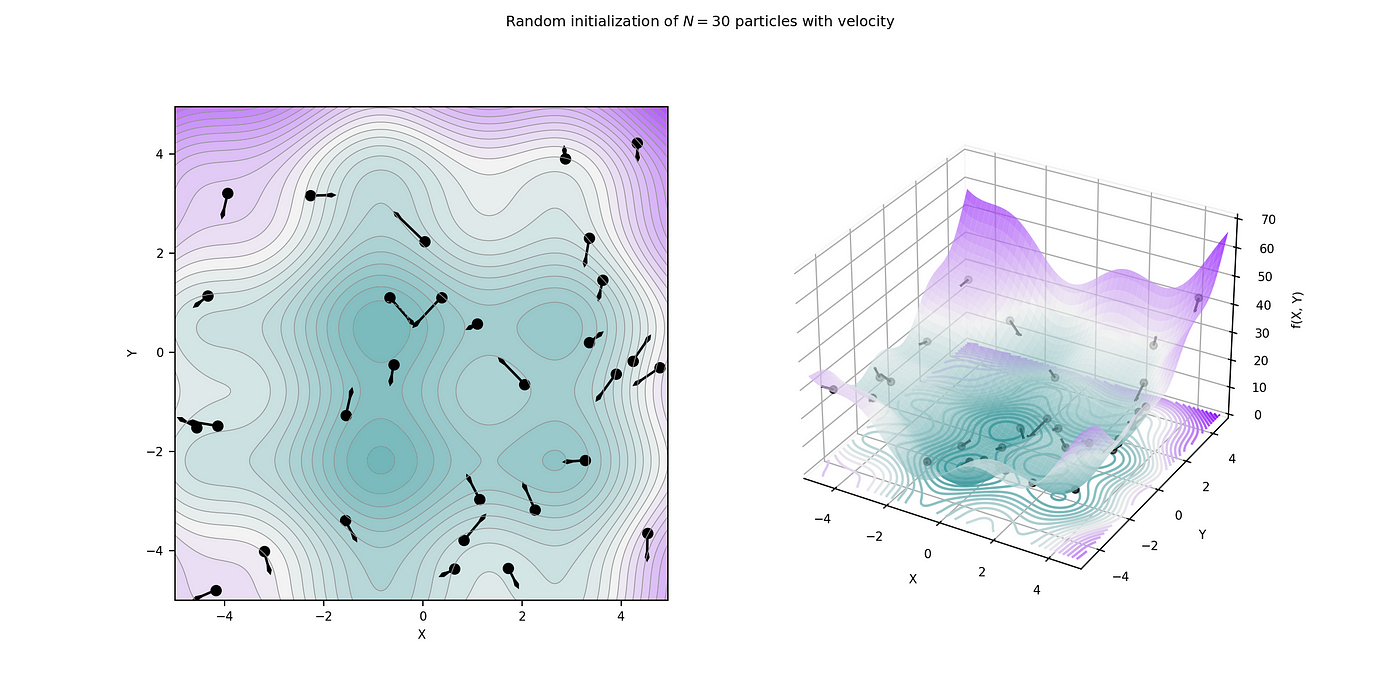
\includegraphics[scale=0.35]{pso.png}
	\caption{Illustration of particles moving in a 3D space}
\end{figure}

PSO has also a binary implementation called Binary Particle Swarm Optimization (BPSO).
The basic principles of BPSO are similar to those of standard PSO, with particles searching for the optimal solution through iterative updates of their positions and velocities. However, in BPSO, the binary representation of the particle's position is manipulated using binary operators such as bitwise AND, OR, and NOT, instead of arithmetic operations used in continuous PSO. \cite{kennedyDiscreteBinaryVersion1997}

The binary version suits feature selection since the binary values represent whether a feature is present or not in the subest of the most relvevant features.

We present here the updated equations for BPSO, the main difference being that here the position of the particle can either be 1 or 0. \cite{abdullahEEGChannelSelection2022}


\begin{align}
S(v) &= \left(1+e^{-v}\right)^{-1} \\
x_{k+1}^i &=1 \:\:\:\:\:\: \text { if } \tau<S\left(v_{k+1}^i\right) \\
x_{k+1}^i &=0 \:\:\:\:\:\: \text { if } \tau>S\left(v_{k+1}^i\right),
\end{align}

With v defined as previously in PSO, and S being a logistic function that varies from 0 to 1.
We decide if the position of the i-th particle is 1 or 0 depending on the $\tau$.
There are also multi-objective versions for both PSO and BPSO called Multi-Objective Particle Swarm Optimization (MOPSO) and Binary Multi-Objective Particle Swarm Optimization respectively (BMOPSO). \cite{coellocoelloMOPSOProposalMultiple2002}

\begin{table}[H]
\caption{Accuracy for particle swarm optimization methods}
\begin{tabular}{|c|c|c|c|p{2cm}|c|}
\hline
Methods & Methods' stategy & Classifier &Accuracy&No. of Selected Channels/Total No. of Channels&Dataset\\
\hline
Afghanistan   & AF    &AFG&   004&   004&   004\\
Albania &AL & ALB&  008&   004&   004\\
Algeria    &asdasdsssssssssssasd & DZA&  012&   004&   004\\
Andorra& AD  & AND   &020&   004&   004\\
Angola& AO  & AGO&024&   004&   004\\
\hline
\end{tabular}
\end{table}


\subsection{Other methods}

We will now present a few other methods that are relvant for the idea behind them, the performance on the evaluation metrics or are particularly interesting with regard to future possible developments.

\subsubsection{Min. Redundancy Max. Relevancy (mRMR)}

\subsubsection{Rayleigh coefficient maximization Based Genetic Algorithm}

\subsubsection{Fisher's criterion}

% The aim of channel selection is to select the most discriminative EEG channels from the original 30 channels by applying the Fisher's criterion. The FD features from the 30 channels are concatenated to a feature vector (called data hereafter) of dimension q
% , where q=30
% . Let 𝐱𝑖𝑗∈𝑅𝑞
%  denotes the jth training data of class 𝑖
% , where 𝑖=1,…, 𝑐
% , 𝐦𝑖
%  is the mean of the training data of the ith class, and 𝐦
%  is the mean of the training data from all classes. In this study, we focused on the classification problem in a motor imagery task (resting vs. motor imagery). Thus, 𝑐=2
% . The within-class 𝐒𝑤
%  and the between-class 𝐒𝑏
%  scatter matrices are calculated by

%  \cite{liuMotorImageryEEG2017}

 
% \begin{aligned}
% & \mathbf{S}_w=\sum_{i=1}^c P_i\left(\frac{1}{n_i} \sum_{j=1}^{n_i}\left(\mathbf{x}_{i j}-\mathbf{m}_i\right)\left(\mathbf{x}_{i j}-\mathbf{m}_i\right)^t\right) \\
% & \mathbf{S}_w=\sum_{i=1}^c P_i\left(\frac{1}{n_i} \sum_{j=1}^{n_i}\left(\mathbf{x}_{i j}-\mathbf{m}_i\right)\left(\mathbf{x}_{i j}-\mathbf{m}_i\right)^t\right)
% \end{aligned}

% respectively, where 𝑛𝑖
%  denotes the number of data in the ith class, the superscript ‘t’ stands for the transpose of a matrix, and 𝑃𝑖=𝑛𝑖/∑𝑐𝑗=1𝑛𝑗
%  is the prior probability of the ith class. The class separability for the fth feature (𝑓=1,…,𝑞
% ) can be represented by the Fisher score 𝐹(𝑓)
% As

% \begin{aligned}
% F(f)=\frac{\mathbf{S}_b(f)}{\mathbf{S}_w(f)}, \quad f=1,2, \ldots, q
% \end{aligned}

% where 𝐒𝑏(𝑓)
%  and 𝐒𝑤(𝑓)
%  are the fth diagonal elements of 𝐒𝑏
%  and 𝐒𝑤
% , respectively. The higher the value of 𝐹(𝑓)
%  is, the better the class separability of the feature extracted from the fth channel is. Based on the class separability criterion, we can select 𝑑
%  top channels among the 30 ones. The 𝑑
%  features from the selected channels are concatenated to a feature vector.

\subsubsection{Automatic Channel Selection with Sparse Squeeze and Excitation Blocks (ACS-SE)}


\subsubsection{Auto-encoder}


\subsubsection{Dataset and results}


We wanted to find algorithm that not only performed well on the usual Accuracy-F1Score metrics while reducing the numbers of channels, but also would fit well with our models.
Given the architecture of our ENGNet model, we needed an algorithm to perform channel selectiom that would work with a Neural Network model.
''' expand test case scenario and explain why '''
In addition, given future test case scenarios we also needed an algorithm that could be performed in an "on-line" way, or as close to it as possible.
To summarize we needed:
\begin{itemize}
	\item-online
	\item Cnn ready
	\item good performance on f1-Accuracy
	\item works well with few channels
\end{itemize}

There are many algorithms that reduce noise...  \cite{abdullahEEGChannelSelection2022}
but those are already inside the ENGNet since spatial features ...
Talk about why ASR didn't improve, basically same reason.
Ideally we would select channels, by iterating over all possible subsets of features but too much time.
Particle swarm optimization no, beacuse too much time.
Therefore correlation algorithms, promising and tested with CNN.
Since we already had CNN why not implement a new algorithm that hasn't been well tested that requires to add one layer.
Critical issue could be that generally black but we will discsuss it later.


\chapter{Materials and Methods}
% \label{ch:conclusions}%
This chapter delves deeper into the materials and methods we used to both write the firmware code for the boards of the PNRelay project and to work on the algorithms for the channel selection.
Given the limitations at hand, the focus of our work was to try and solve a list of different issues that came up during the development of the project.
In particular:

\begin{itemize}
	\item Optimization of firmware communication parameters
	\item Safe transmission via BLE
	\item Channel selection
	\item Calculation of dissipated power
	\item Memory management
	\item Reversible transmission
\end{itemize}

We will divide this chapter into two main parts: one that is related to the firmware and the hardware aspects, one that is related to the channel selection algorithms.
These two parts have been carried on for the majority of our work indipendently and despite the common goal share little to no similarities as far as materials and methods go.

\section{Channel selection}

\subsection{Newcastle Dataset}

The Newcastle Dataset presents the recording of ENG signals of three different Sprague Dawley rats in response to mechanical sensory stimulation.
To each of these rats a 16-contact cuff electrode was chrirurgically inserted and placed around the sciatic nerve in a distal position, close to where the nerve branches into its peroneal, sural, and tibial components.
The data include ten different kinds of stimulation grouped into the three main categories of stimulation: Nociception, Proprioception and Touch.

\textbf{Nociception} \quad This class represents the pinching at two different points in the foot: the heel and the outer toe.
These two nociceptive stimuli were elicited through manually operated tweezers with a Force Sensitive Resistor sensor connected to them in order to standardize the force applied, the duration and the synchronization in order to replicate the stimulus with precision.

\textbf{Proprioception} \quad This class of stimulus includes six different kinds of applied stimulation, each of them correspond to a different angle of ankle flexion, considered either dorsiflexion or plantarflexion.
Ther is three different angles for dorsiflexion with positive degrees (-10°, -20°, -30°) and three different angles for plantarflexion with positive degrees (+10°, +20°, +30°).
The angle measurement is relative to the neutral position of the ankle.
This movements were obtained by pushing the hind paw of the rats with a bar, with a flex sensor to detect precisely the movement in order to standardize the procedure.
Each movement was performed and then the position at the specific angle was kept for three seconds, then the neutral position was restored.

\textbf{Touch} \quad This class represents two different stimuli based on the force of the touch: 0.1 Kg and 0.3 Kg.
These two stimuli were elicited using Von Frey(VF) fibers, once again with a flex sensor in order to synchronize the procedure and standardize it by unfolding as the motor pushed the VF fiber to touch the hind paw.

While these ENG recordings were taken the rats were anesthetized in order to eliminate any possible EMG voluntary activity. The signals were captured at a frequency of 30 kHz and then digitally flitered between 0.25 and 5kHz.
Each of the different stimuli previously presented was applied 50 times, producing 500 sampples in total for each rat. [davide]

\subsubsection{Preprocessing}

\begin{figure}[H]
	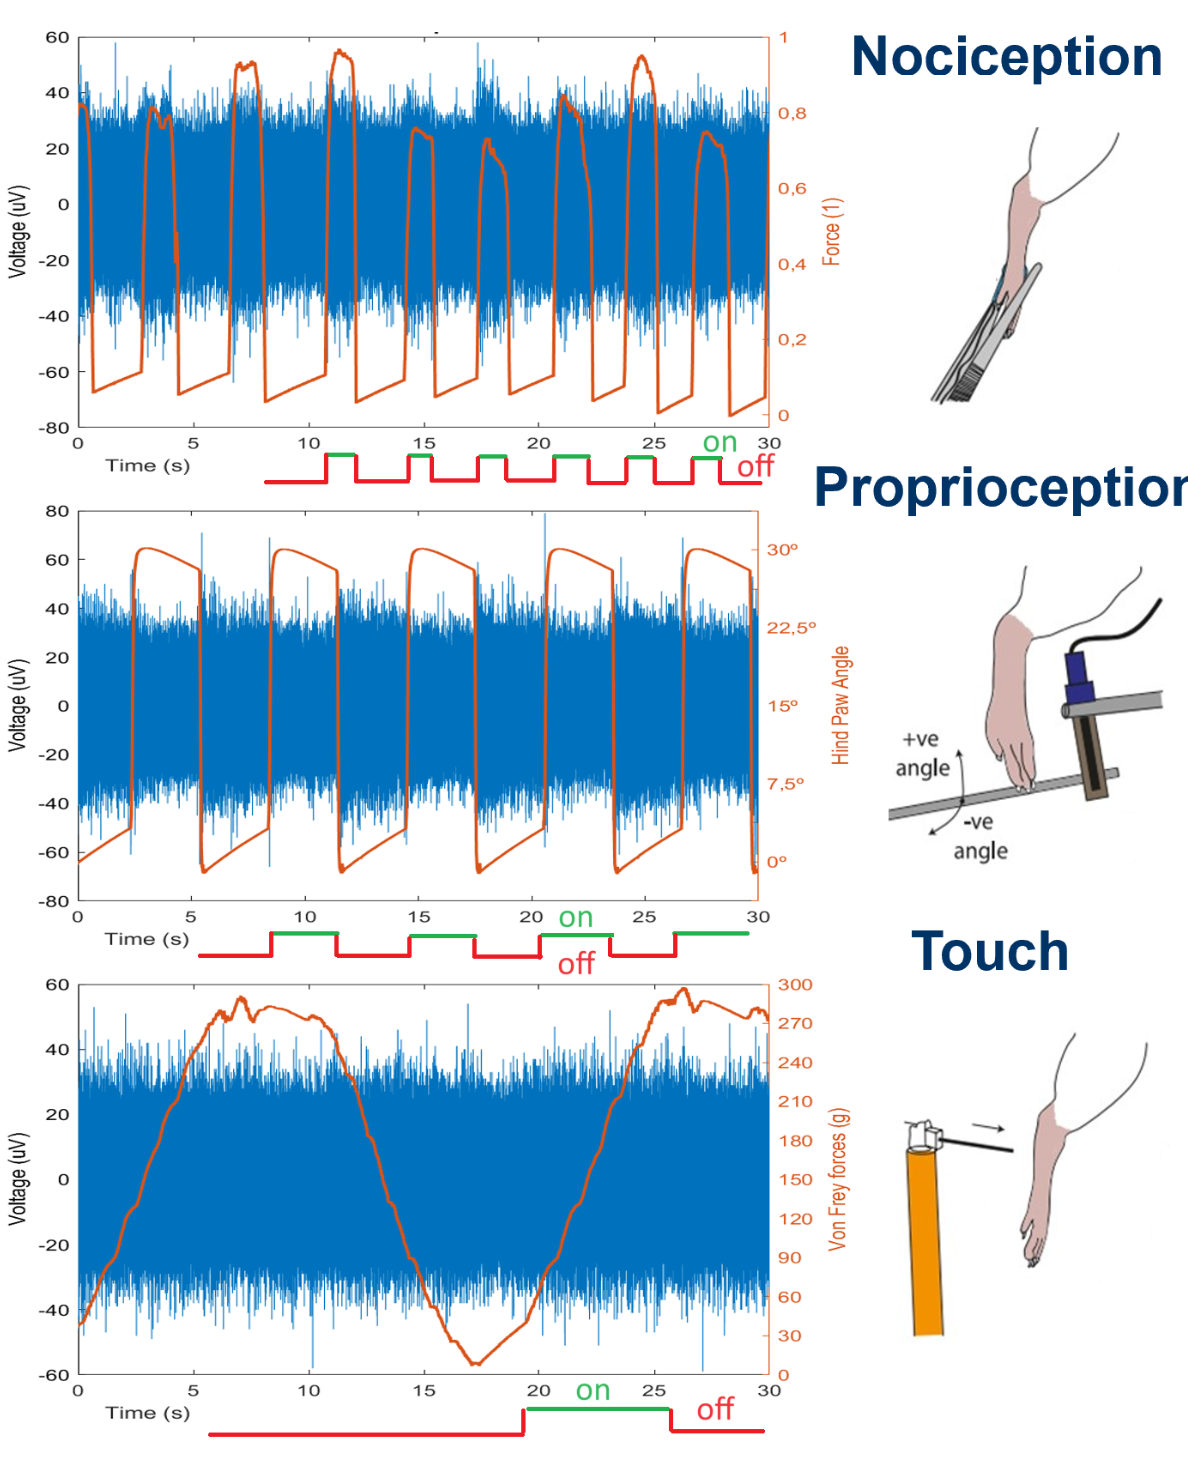
\includegraphics[scale=0.4]{acquiredStimuli.png}
	\centering
	\end{figure}


\begin{figure}[H]
	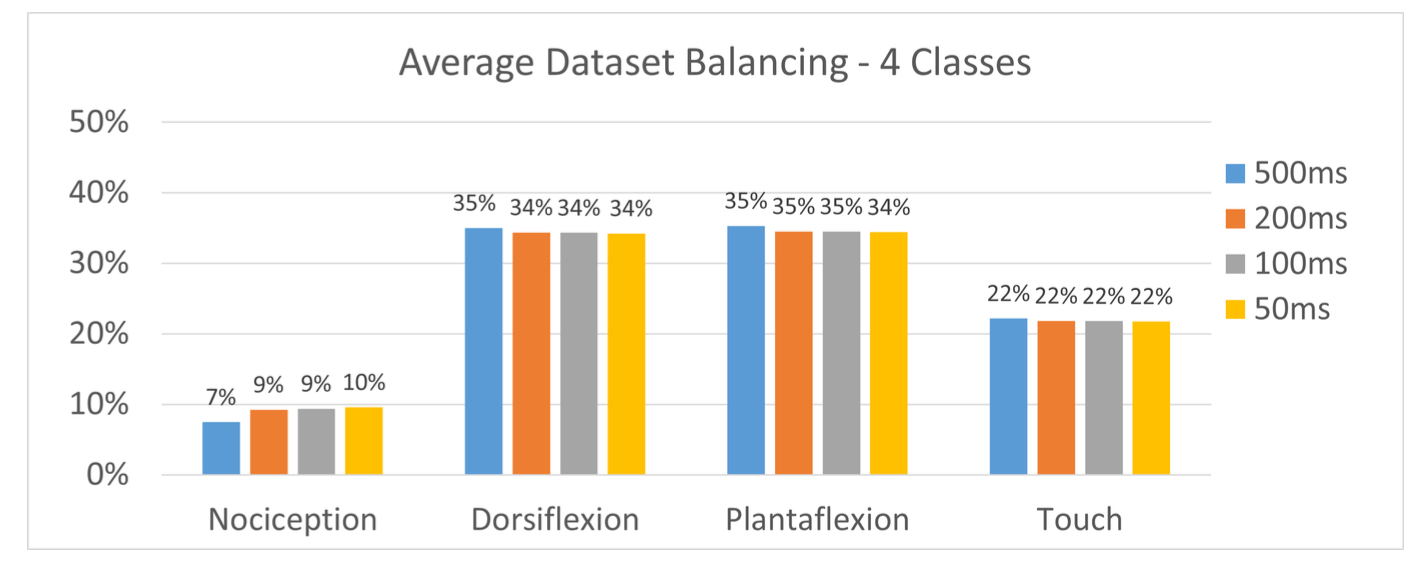
\includegraphics[scale=0.4]{balanceClass.png}
	\centering
	\end{figure}
	

\subsection{Channel selection algorithms}

As stated previously, the focus of the channel selection algorithm is to reduce the number of channels that need to be transmitted in order to perform the classification of the signals properly.
In particular as we will see better in the results chapter, we consider as an acceptable loss anything better than a 5 percentage points drop in F1-Score which is our core metric for the evaluation of the classification.

\subsubsection{Test-case conditions}

Poeple + setup +time + how signals come ....

Our dataset as explained in the previous section comprises 16 channels.
Once condition that needs to be specified is that in order to simulate real test-case condtions on people, the channels may not come in batches of 16 channels, but as 8 channels + 8 channels.
Therefore we performed our algorithms of evaluation not only on the whole 16 channels, but also on 8 channels, then other 8 channels and then cross-checked the results.
In addition we have also tried a different approach we will explain later that due to its characteristic of being implemented at training time could not be applied to both 16 channels and 8 + 8 channels but requiered the 16 channels

\subsubsection{Correlation based algorithms}

These methods help identifying which subsets of channels is the most relevant by defining a correlation metric and ranking higher those channels that show stronger similarities between them according to the metric.
As shown in Chapter 3 there are more than a few examples of correlation based algorithms for channel selection.
We focus here on the ones we used extensively during our work: Cross-Correlation Based Discriminant Criterion (XCDC) and our own iteration.
We will now present again the structure of the algorithms explaining the steps and our overall pipeline for the channel selection.

\subsubsection{Cross-Correlation Based Discriminant
Criterion (XCDC)}

The goal of the XCDC is to return a metric that correctly evaluates ths signals based on same-channel correlation.
The steps required are as follows:
\begin{itemize}
	\item XCDC between same-channel signals
	\item Score for same-class correlation
	\item Score for different-class correlation
	\item Final score
\end{itemize}

First of all, we take 48 samples for each one of the four classes we described in the dataset section.

\begin{itemize}
	\item 48 Nociception samples
	\item 48 Plantaflexion samples
	\item 48 Dorsiflexion samples
	\item 48 Touch samples
\end{itemize}

Then we split each of the 48 samples in two batches of 24 samples represented in the figure as Column I and Column II.
We split each of the columns in 3 batches of 8 samples.
We now proceed to perform XCDC between the batches of Column I and Column II as represented in Figure 

\begin{figure}[H]
	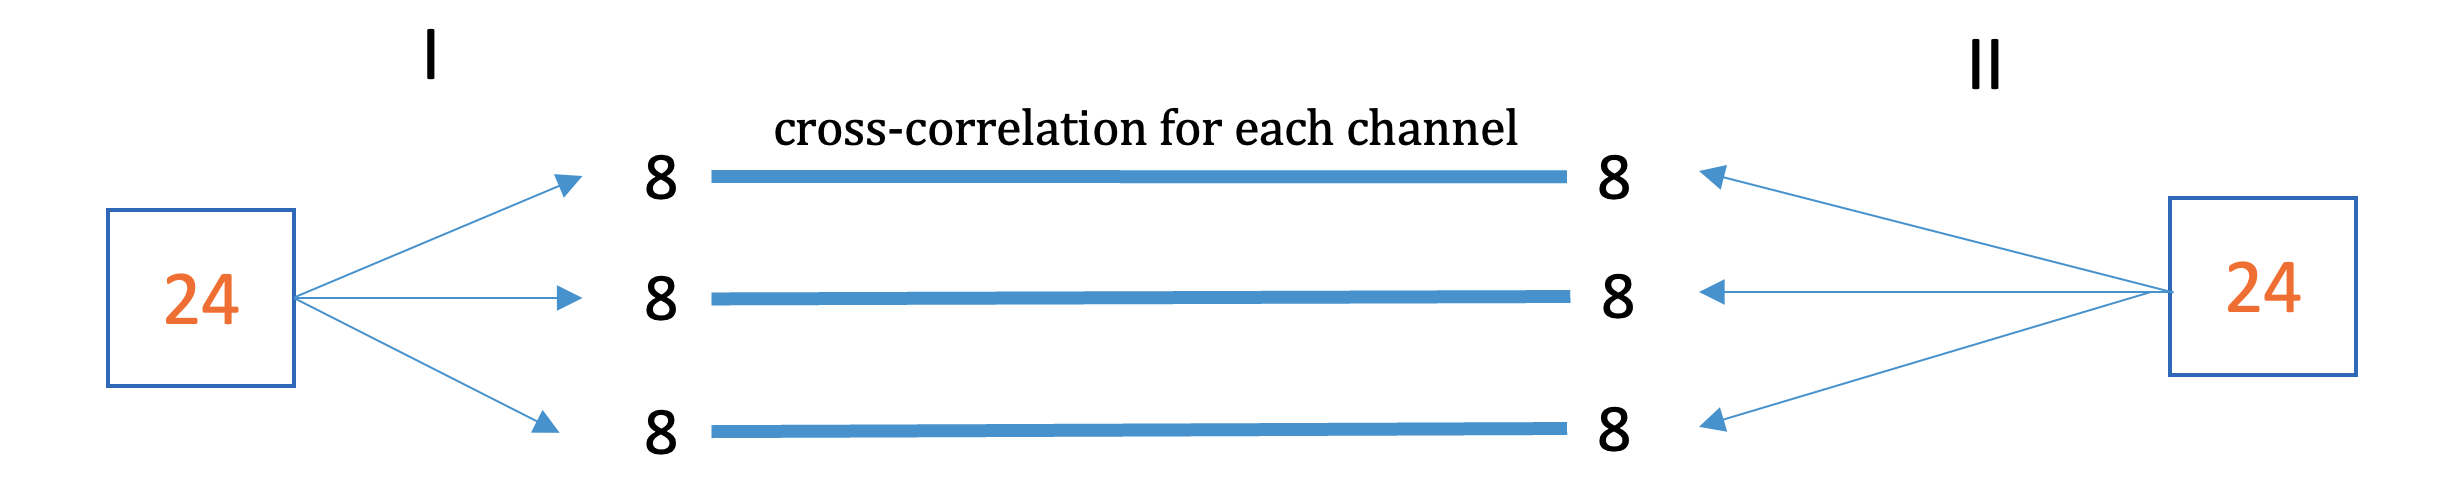
\includegraphics[scale=0.4]{dataSplit.png}
	\centering
	\end{figure}



	\begin{figure}[H]
		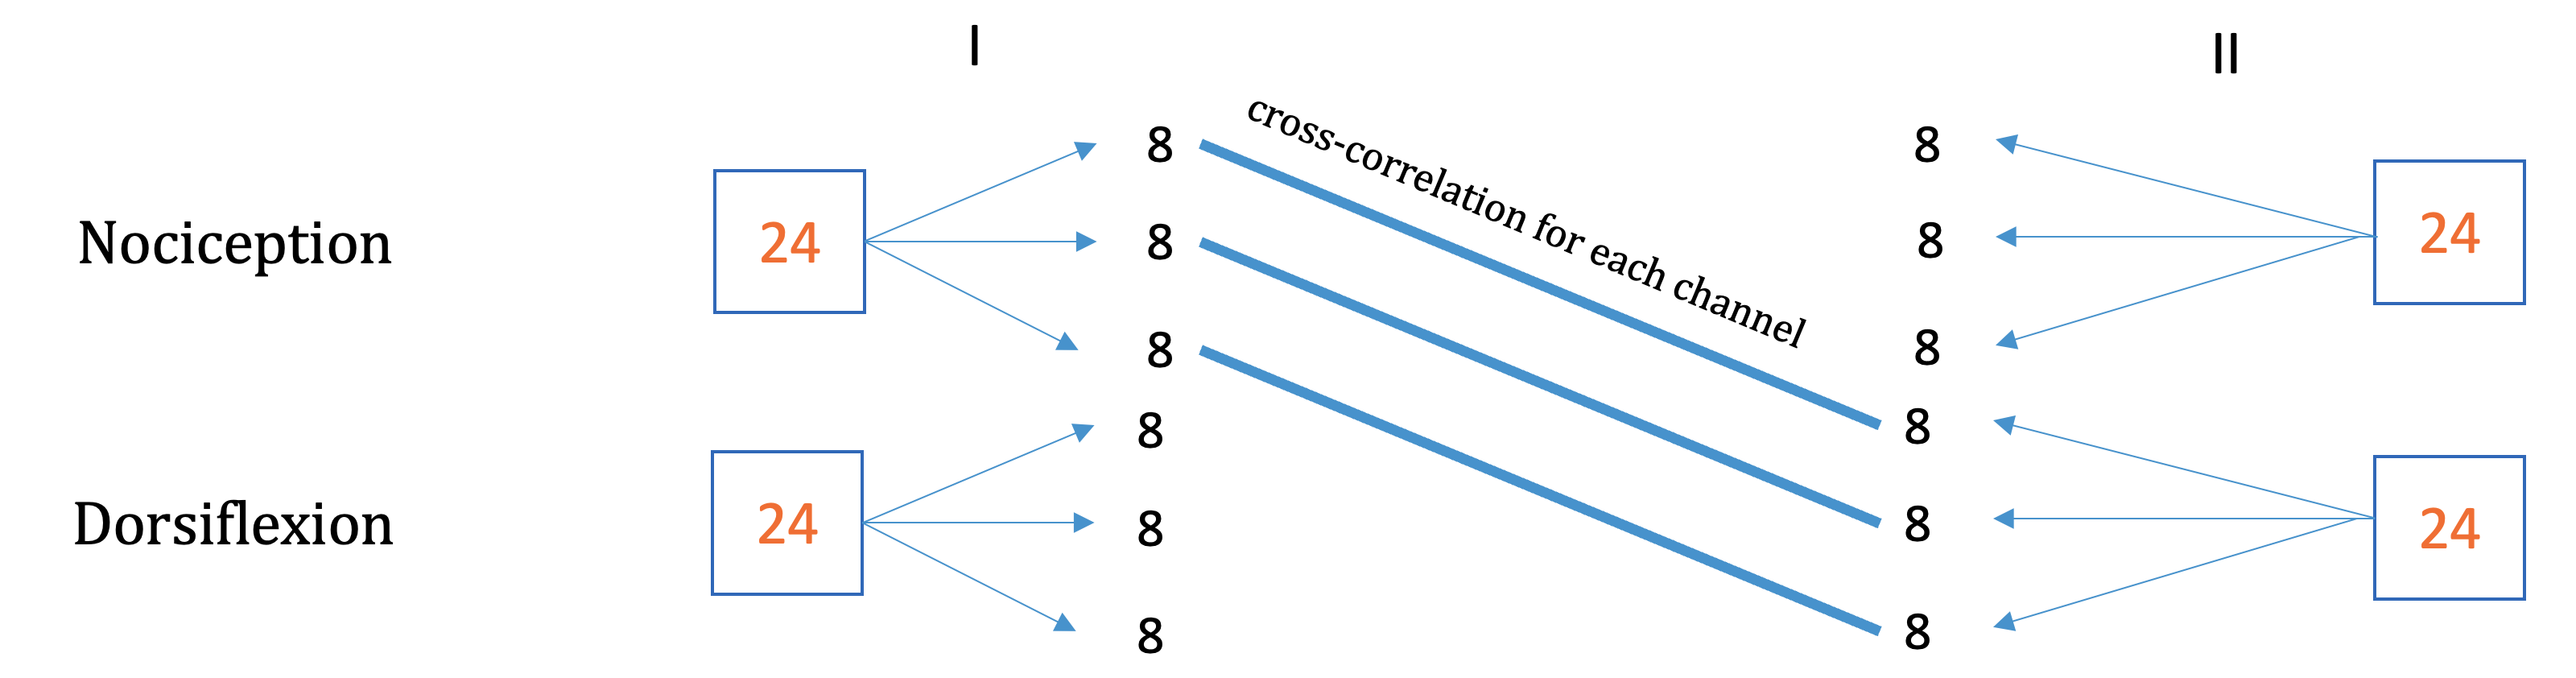
\includegraphics[scale=0.4]{scoreDifferentClass.png}
		\centering
		\end{figure}
	


Given two finite discrete time series $x(i)$ and $y(j)$
(i $\epsilon$ $[0, 1, . . . , n - 1]$, j $\epsilon$ $[0, 1, . . . , m - 1]$, $m \geq n$),
their cross-correlation series is given as follows:

\begin{align}
	 r_{xy}(k) = \sum_{i=0}^{n-1}x(i)y(i + k), k = 0,1,...,m-n+1
	\label{eq:XCDC1}
\end{align}

where x and y are EEG signals of length T (m=n=T). \\ 
Zero-padding is performed at both sides of y so that the length of the cross-correlation series is the same of the original signals. \\
We apply the cross-correlation formula to the signals x and y, but we must firstly apply z-score normalization to account for the effect of signal amplitudes on cross-correlation.

\begin{align}
	\tilde{x_i} = \frac{x_i - \bar x_i}{\sigma_{x_i}}
   \label{eq:XCDC3}
\end{align}


Then, the similarity between x and y is measured with the following formula:

\begin{align}
	S(x,y) = \max(r_{x\hat{y}(k)}), k=0,1,..., T - 1 
   \label{eq:XCDC2}
\end{align}

with $\hat{y}$ being y with zero-padding.
where $x_i$ is the signal of the i-th trial collected from our channel of interest. $\bar{x_i}$ and $\sigma{x_i}$ are
the mean and standard deviation of $x_i$ respectively.
Having defined the function $S$ we now define the within-class similarity $R_w$ and betweenclass dissimilarity $R_b$ which are obtained as follows:

\begin{align}
	R_w = \mathbf{mean}(S(\tilde{x_i}\tilde{x_j}| c_i = c_j))
   \label{eq:XCDC4}
\end{align}

\begin{align}
	R_b = -\mathbf{mean}(S(\tilde{x_i}\tilde{x_j}| c_i \neq  c_j))
   \label{eq:XCDC5}
\end{align}

where $c_i$ is the class label of the i-th trial. The discriminant score D is then defined as follows:

\begin{align}
	D = \lambda R_w + (1-\lambda)R_b
   \label{eq:XCDC6}
\end{align}

in which $\lambda$ is a weighting hyperparameter to be tuned empirically.
Channels are ranked in a descending order according to their discriminant score D after obtaining D for every channel using.

\subsubsection{Our approach}

Since XCDC evaluates same-channel metrics, we wanted to iterate over this approach and create a metric that could evaluate how much different channels carried the same amount of information.
Let us delve deeper in the actual differences.
The steps of the algorithm are as follows:

\begin{itemize}
	\item XCDC between same-channel signals
	\item Discard noisy signals
	\item Cross-correlation between different-channel signals
	\item Score for same-class correlation
	\item Score for different-class correlation
	\item Final score
\end{itemize}


Therefore, compared to the previous algorithm, we don't correlate a channel with itself, we correlate it with each of the other 15 channels.
Therefore we now have 15 times the amount of data we had with the first iteration.
%-------------------------------------------------------------------------
%	BIBLIOGRAPHY
%-------------------------------------------------------------------------

\addtocontents{toc}{\vspace{2em}} % Add a gap in the Contents, for aesthetics
\bibliography{Thesis_bibliography} % The references information are stored in the file named "Thesis_bibliography.bib"

%-------------------------------------------------------------------------
%	APPENDICES
%-------------------------------------------------------------------------

\cleardoublepage
\addtocontents{toc}{\vspace{2em}} % Add a gap in the Contents, for aesthetics
\appendix
\chapter{Appendix A}
If you need to include an appendix to support the research in your thesis, you can place it at the end of the manuscript.
An appendix contains supplementary material (figures, tables, data, codes, mathematical proofs, surveys, \dots)
which supplement the main results contained in the previous chapters.

\chapter{Appendix B}
It may be necessary to include another appendix to better organize the presentation of supplementary material.


% LIST OF FIGURES
\listoffigures

% LIST OF TABLES
\listoftables

% LIST OF SYMBOLS
% Write out the List of Symbols in this page
\chapter*{List of Symbols} % You have to include a chapter for your list of symbols (
\begin{table}[H]
    \centering
    \begin{tabular}{lll}
        \textbf{Variable} & \textbf{Description} & \textbf{SI unit} \\\hline\\[-9px]
        $\bm{u}$ & solid displacement & m \\[2px]
        $\bm{u}_f$ & fluid displacement & m \\[2px]
    \end{tabular}
\end{table}

% ACKNOWLEDGEMENTS
\chapter*{Acknowledgements}
Here you might want to .


\cleardoublepage

\end{document}
